\documentclass[12pt,a4paper,openright,twoside]{book}
\usepackage[utf8]{inputenc}
\usepackage{disi-thesis}
\usepackage{code-lstlistings}
\usepackage{notes}
\usepackage{shortcuts}
\usepackage{acronym}
\usepackage{float}
\usepackage{comment}

\renewcommand{\lstlistlistingname}{Elenco dei listati}
\renewenvironment{acknowledgements}
  {\chapter*{Ringraziamenti}}
  {}



\raggedbottom{}
\school{\unibo}
\programme{Corso di Laurea in Ingegneria e Scienze Informatiche}
\title{Progettazione di un configuratore di vendite}
\author{Mattia Cavina}
\date{\today}
\subject{Basi di dati}
\supervisor{Prof.ssa Annalisa Franco}

\session{III}
\academicyear{2025--2026}

% Definition of acronyms
\acrodef{CPQ}{Configure, Price, Quote}
\acrodef{ERP}{Enterprise Resource Planning}
\acrodef{CRM}{Customer Relationship Management}
\acrodef{PLM}{Product Lifecycle Management}
\acrodef{vm}[VM]{Virtual Machine}
\acrodef{SSIS}{SQL Server Integration Services}
\acrodef{Cepi}{Cepi S.p.A.}
\acrodef{ETO}{Engineering To Order}
\acrodef{SRP}{Single Responsibility Principle}
\acrodef{DB}{Database}
\acrodef{NAT}{Network Address Translation}
\acrodef{VPN}{Virtual Private Network}
\acrodef{TCP}{Transmission Control Protocol}
\acrodef{IP}{Internet Protocol}
\acrodef{DTO}{Data Transfer Object}
\acrodef{EF Core}{Entity Framework Core}
\acrodef{DRY}{Don't Repeat Yourself}
\acrodef{ORM}{Object-Relational Mapping}
\acrodef{LINQ}{Language INtegrated Query}
\acrodef{MVVM}{Model View ViewModel}
\acrodef{UX}{User Experience}
\acrodef{AD}{Active Directory}
\acrodef{SSMA}{SQL Server Migration Assistant}
\acrodef{SSIS}{SQL Server Integration Services}
\acrodef{ER}{Entity Relationship}
\acrodef{TCP/IP}{Transmission Control Protocol/Internet Protocol}
\acrodef{AI}{Artificial Intelligence}
\acrodef{IA}{Intelligenza Artificiale}
\acrodef{LAN}{Local Area Network}
\acrodef{CRUD}{Create Read Update Delete}
\acrodef{API}{Application Programming Interface}
\acrodef{RAM}{Random Access Memory}
\acrodef{CPU}{Central Processing Unit}
\acrodef{ID}{Identifier}
\acrodef{OOP}{Object-Oriented Programming}
\acrodef{RA}{Richiesta di assistenza}
\acrodef{BOM}{Bill Of Material}
\acrodef{SQL}{Structured Query Language}
\acrodef{HTML}{HyperText Markup Language}
\acrodef{CSS}{Cascading Style Sheets}
\acrodef{JS}{JavaScript}
\acrodef{1NF}{Prima Forma Normale}
\acrodef{2NF}{Seconda Forma Normale}
\acrodef{3NF}{Terza Forma Normale}
\acrodef{DI}{Dependency Injection}
\acrodef{SVG}{Scalable Vector Graphics}

\acrodef{UT}{Ufficio Tecnico}
\acrodef{UTE}{Ufficio Tecnico Elettrico}
\acrodef{PM}{Project Manager}
\acrodef{PE}{Project Engineer}

\hypersetup{
    colorlinks=true,
    urlcolor=blue,
    linkcolor=cyan,
    citecolor=red
}

\mainlinespacing{1.241} % line spacing in mainmatter, comment to default (1)

\begin{document}

\frontmatter\frontispiece{}

%Abstract
\begin{abstract}
    Il presente lavoro di tesi descrive la progettazione e lo sviluppo di un software full-stack
    a supporto del reparto commerciale di Cepi S.p.A.\cite{Cepi}, 
    contesto aziendale in cui l'autore opera come dipendente.
    L'azienda metalmeccanica forlivese è specializzata nella produzione di impianti
    di stoccaggio con logica \ac{ETO}.
    Il sistema realizzato, si qualifica come soluzione \ac{CPQ}
    consentendo la configurazione del prodotto, la generazione di offerte
    commerciali e la conseguente stipula dei contratti.
    L'elaborato copre l'intero ciclo di vita del progetto: dall'analisi
    dell'as-is e la raccolta dei requisiti, fino alla modellazione del database relazionale e
    all'implementazione del software.
    La gestione dei dati è affidata a Microsoft SQL Server, mentre l'applicativo è stato sviluppato
    in linguaggio \csharp{} su framework \dotnet{}. La scelta di questo ecosistema risponde all'esigenza di
    realizzare un'applicazione cross-platform installabile in locale, requisito essenziale per garantire la piena
    operatività offline anche in contesti privi di connettività di rete.
    L'interfaccia utente è stata infine implementata sfruttando il framework \maui{}.
\end{abstract}


%----------------------------------------------------------------------------------------
\tableofcontents
\listoffigures     % (optional) comment if empty
\lstlistoflistings{}  % (optional) comment if empty
\listoftables{}      % (optional) comment if empty
%----------------------------------------------------------------------------------------

\mainmatter{}

\chapter{Introduzione}\label{chapter:introduction}
Il progetto di tesi è volto alla progettazione ex-novo del programma di vendita dell'azienda Cepi S.p.A.,
azienda con una produzione di tipo \ac{ETO} specializzata nella progettazione di impianti di stoccaggio custom.
La tipologia di produzione \ac{ETO} ha portato ad un profondo studio della situazione odierna, delle sue esigenze attuali
e future tenendo aperte le possibilità di ampliamenti.
L'analisi ha comportato un sostanziale lavoro di programmazione e raccolta dati per coprire nel modo più
ampio i bisogni aziendali.
Questa prima fase è stata condotta inizialmente attraverso la selezione di figure chiave scelte per mansione e/o ruolo,
che potessero
dare una visione dei bisogni del proprio o altrui reparto e successivamente sottoponendole ad interviste.
Sono state condotte 14 interviste, di cui 8 in modalità vis a vis, mentre le restanti 6 attraverso la dimostrazione
dell'attuale applicativo utilizzato.
Il risultato delle interviste condotte, ha fatto emergere attuali e nuove necessità architetturali da affrontare
come il cross-platform, l'utilizzo offline del database e la necessità di costruire offerte in modo più agile e strutturato.
Questa prima fase ha inoltre sottolineato come il progetto non debba solo sostituire l'attuale sistema,
ma debba inserirsi in un contesto di rinnovamento più ampio, coordinandosi con altri programmi aziendali e relativi database in ottica ``\ac{SRP}''
eleggendo dei master data che siano i soli responsabili della creazione di certi dati.
Lo \ac{SRP} ha plasmato notevolmente la costruzione del database ricreando, dove possibile,
le strutture pre-esistenti da cui si necessitava recuperare i dati mediante reverse engineering.
L'intero sistema è stato pensato per appoggiarsi all'infrastruttura esistente aziendale come SQL Server\cite{SQLServer}.
Sopra di esso sono state progettate delle logiche di flessibilità e ampliamento dinamico studiando accuratamente le relazioni tra le tabelle.
Si è reso necessario cercare e scegliere inoltre un framework per la parte grafica che potesse
soddisfare il deployment cross-platform. Questo requisito è emerso in modo chiaro dalle interviste,
in quanto ci sono situazioni
in cui il personale aziendale si trova a dover lavorare in mobilità, come le fiere di settore.
La costruzione delle interfacce grafiche è stata supportata dal sito ``Figma''\cite{Figma}
che ha permesso una progettazione %vedere se citarlo% 
in ottica mobile first.
La scelta accurata dei framework e delle strutture dati nella fase iniziale
ha pesato molto in termini di tempo e progettazione,
per garantire al richiedente un sistema che non rischiasse né il debito tecnico,
né la preclusione a sviluppi futuri.
La pianificazione dei primi test con gli utenti, dei rilasci delle demo e del metodo di progettazione è
stata cruciale per dettare tempi e priorità degli item. 
L'obiettivo era coprire in modo esaustivo almeno il core del progetto.


\chapter{Situazione As-Is}\label{chapter:AsIs}
\section{Premessa}
La situazione infrastrutturale aziendale è stata studiata dall'autore nel corso del tirocinio formativo.
La raccolta dei dati è stata svolta mediante interviste e studio dell'attuale sistema informatico.
Nelle sezioni che seguono verrà introdotto brevemente l'As-Is.

\section{Situazione infrastrutturale aziendale}
L'infrastruttura informatica aziendale si appoggia su server fisici allocati internamente e gestiti mediante Active Directory.
I server fisici sono, a loro volta, virtualizzati per gestire separatamente le memorie in base alla finalità
garantendo isolamento delle informazioni e permessi di accesso.
Ogni reparto ha accesso a determinati server virtuali in cui gestisce in autonomia i propri contenuti.
I database dei principali programmi sono gestiti all'interno di un server dedicato dove è installato un motore
\sqlserver{}\cite{SQLServer}.
I principali database aziendali sono:
\begin{itemize}
    \item \textbf{Ad\-Hoc\cite{Ad-Hoc}:} l'\ac{ERP} aziendale, programma che gestisce le attività aziendali come gli approvvigionamenti e la movimentazione dei prodotti,
          le vendite, le fatturazioni nonché i cicli produttivi.
    \item \textbf{Fusion\cite{Fusion}:} il \ac{PLM} aziendale, programma volto alla gestione dei prodotti meccanici, dalla loro creazione
          all'archiviazione dei disegni con relative distinte dei componenti.
          Altre funzioni applicate sui prodotti sono la gestione delle revisioni o versionamenti, ed infine la loro fine produzione.
    \item \textbf{BombConfine:} database ponte tra i database esterni e quello dell'\ac{ERP}. All'interno sono presenti tabelle
          di frontiera scritte da programmi esterni e che il gestionale usa per importare i dati.
\end{itemize}
La sicurezza aziendale è sostenuta da \ac{NAT} e Firewall che impediscono
l'accesso dall'esterno se non tramite \ac{VPN}. % fare acronimi
L'infrastruttura aziendale è visibile in figura~\ref{fig:Infrastruttura aziendale}.
\begin{figure}[H]
    \centering
    \fbox{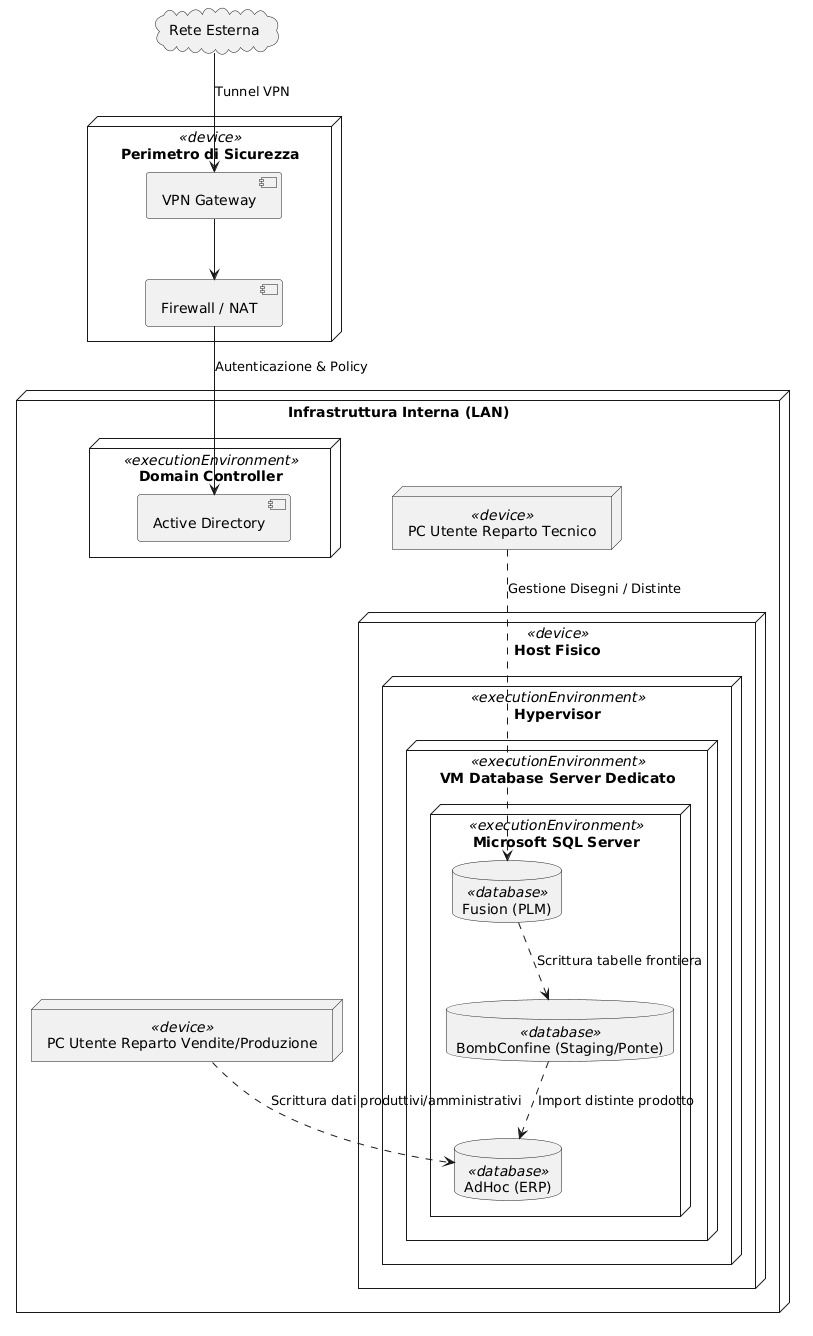
\includegraphics[width=0.8\linewidth]{figures/InfrastrutturaAziendale.png}}
    \caption{Schema infrastruttura aziendale}\label{fig:Infrastruttura aziendale}
\end{figure}
\section{Attuali software utilizzati}
Nel capitolo precedente abbiamo fatto cenno ai database ed ai relativi programmi che gestiscono quanto concerne l'\ac{ERP}
e il \ac{PLM}.
Per quanto riguarda le vendite, punto focale dell'intervento richiesto, l'azienda utilizza attualmente
un'applicazione sviluppata internamente. L'attuale sistema sviluppato in Access, programma della suite Microsoft Office,
comprende al suo interno sia il frontend che il backend.
Il software è stato implementato circa 30 anni fa ed ha subito numerosi aggiornamenti e
modifiche nel tempo per adattarsi alle esigenze commerciali e all'evoluzione del
mercato. L'applicazione consente di creare, modificare e gestire i contratti con i
clienti, includendo funzionalità quali la gestione degli sconti, la personalizzazione
delle offerte e la stampa dei documenti. Tuttavia, nonostante le funzionalità implementate,
il software presenta significative criticità che ne limitano l'efficienza e
l'usabilità, come confermato dalle interviste condotte con gli utenti. Tali criticità
includono instabilità operativa, mancanza di standardizzazione, codifiche obsolete,
difficoltà negli aggiornamenti di prezzo e assenza di integrazione con altri sistemi
aziendali. Di conseguenza, è indispensabile sviluppare un nuovo programma
che affronti tali problematiche e migliori l'esperienza degli utenti,
preservando nel contempo le funzionalità essenziali del sistema attuale.
Il programma Access è stato fondamentale in questi anni per l'utilizzo in zone offline.
Questa funzionalità è stata favorita dalla natura del programma stesso,
il quale racchiude in un solo file database e frontend,
copiandolo in locale e sincronizzandolo una volta tornati in sede.

\section{Organizzazione aziendale e flussi di lavoro}
Il flusso lavorativo è risultato non essere un aspetto secondario nello sviluppo richiesto.
Esso si deve interporre tra il reparto commerciale, ovvero addetti alle vendite,
i reparti progettuali e produttivi come uffici tecnici, logistica ed amministrazione.
L'attuale flusso di lavoro analizzato pone il reparto commerciale come punto di partenza
dell'intero flusso che arriva fino al post-vendita.
Il contratto, creato da tale reparto, dopo essere stato stipulato viene inviato
al reparto amministrativo che ne importa i dati
all'interno del gestionale.
Simultaneamente esso viene mandato al reparto project manager che lo revisiona tecnicamente in
caso di errori progettuali.
Dopo la revisione tecnica, il contratto viene spedito al reparto logistico che preventivamente verifica
i dati di destinazione ed organizza le spedizioni sulla base del venduto.
Il flusso di lavoro può essere visto in figura~\ref{fig:Flusso di un contratto}.
A causa del sistema obsoleto utilizzato ed il debito tecnico accumulato negli anni, l'attuale sistema è isolato
rispetto ai programmi utilizzati dall'azienda.
Quest'ultimo punto fa parte delle richieste imprescindibili da risolvere.
L'integrazione nell'ecosistema informatico passa prima di tutto dall'unificazione dei codici,
ovvero quelli a listino con i prodotti a gestionale, ma anche creando
un flusso di notifiche tra i vari ambiti.
\begin{figure}[ht]
    \centering
    \fbox{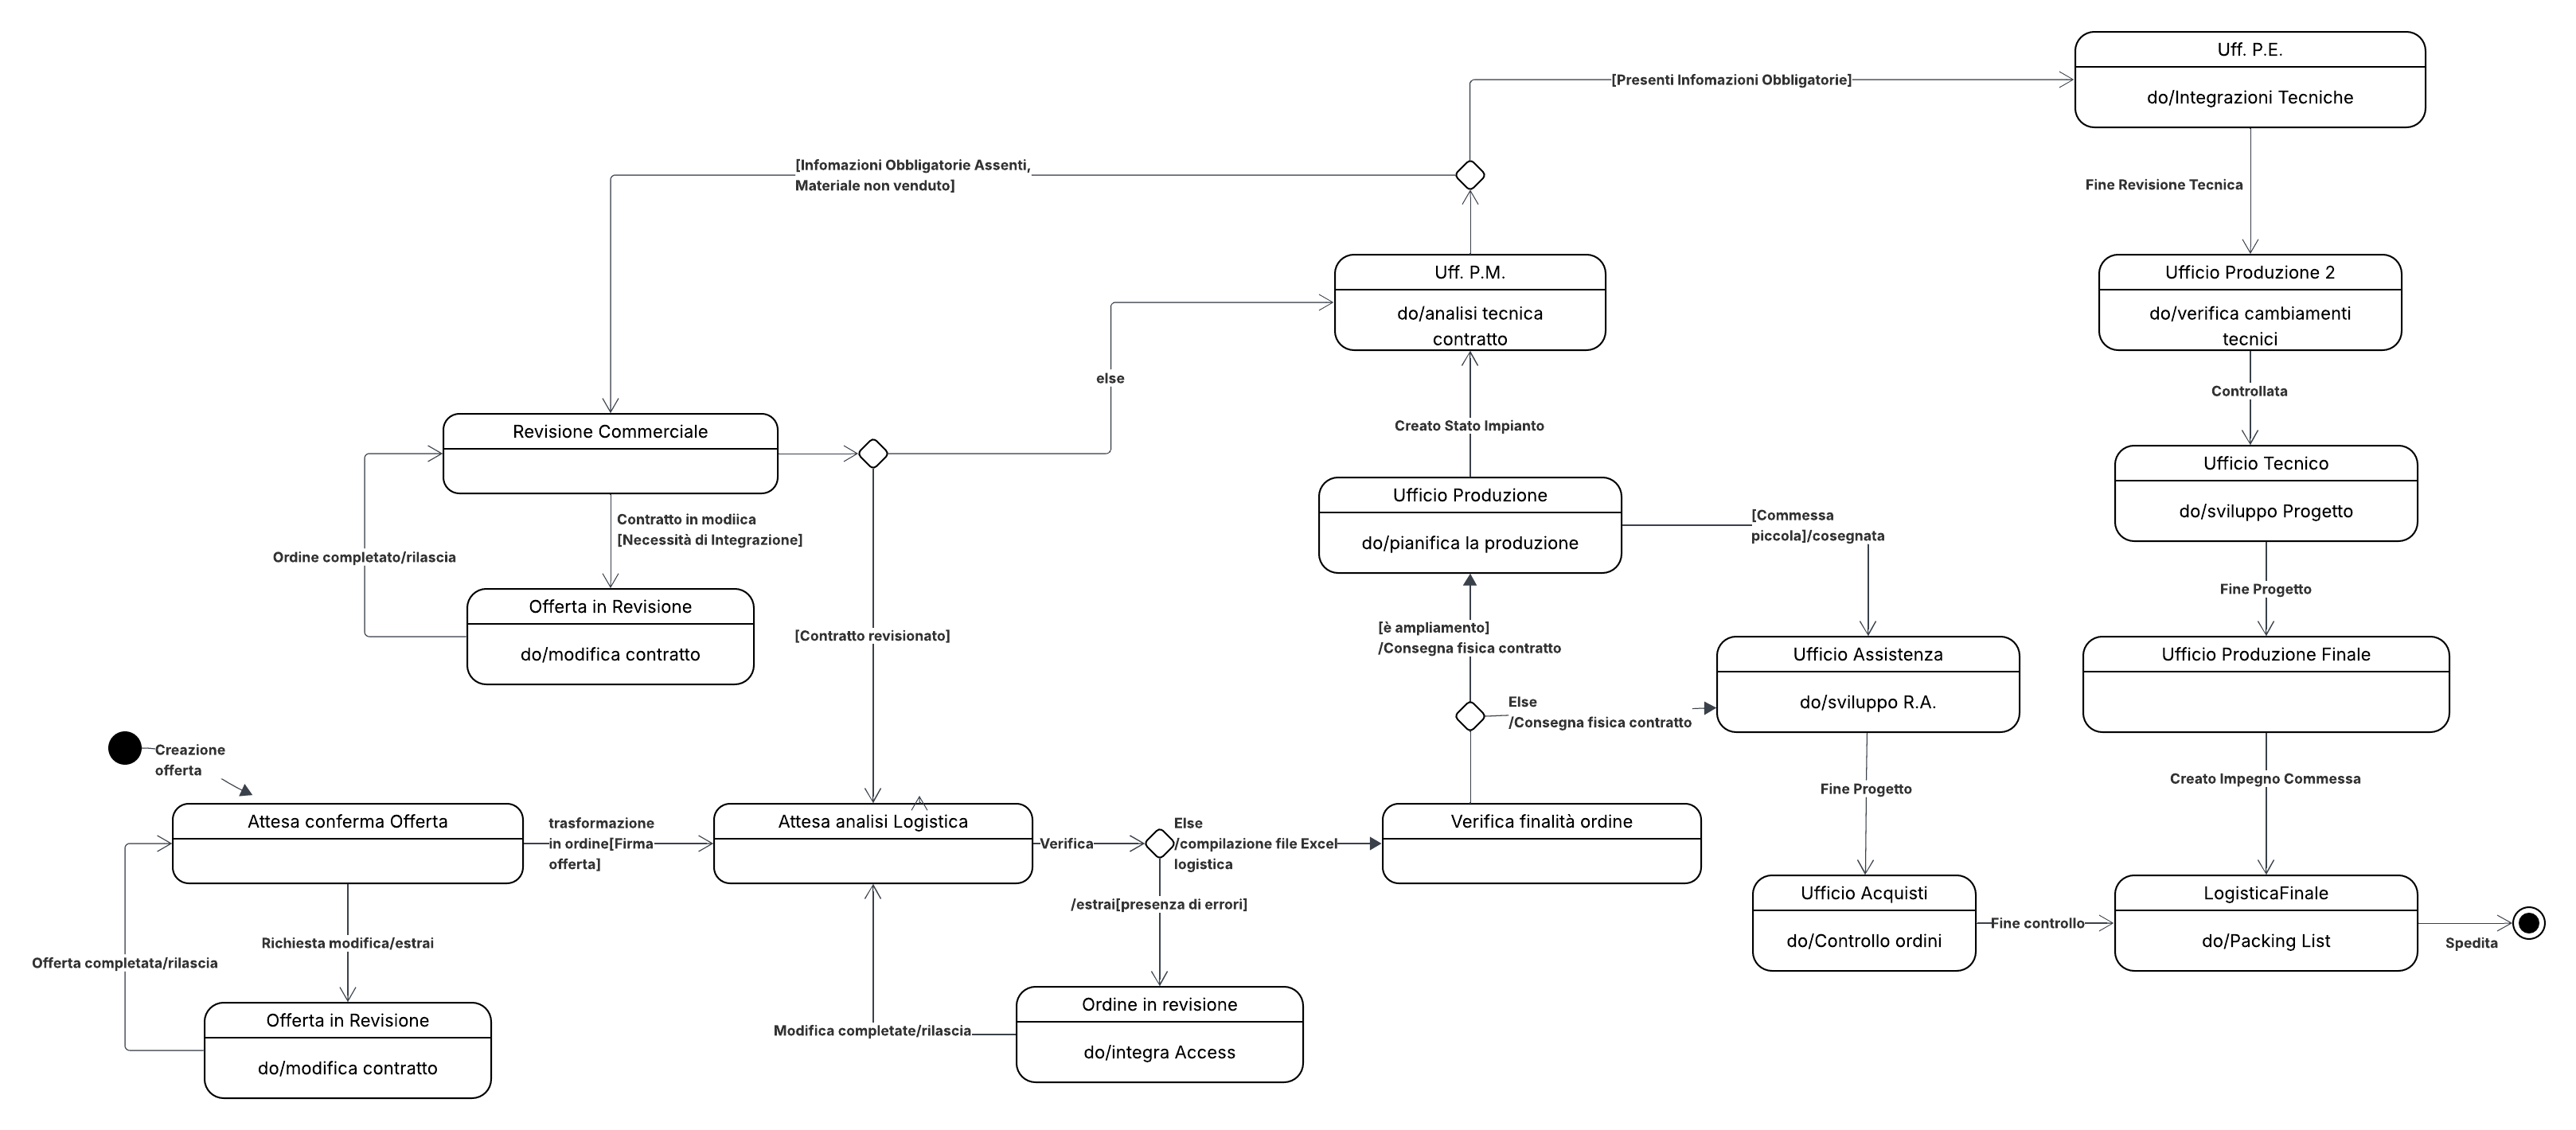
\includegraphics[width=1.2\linewidth, angle=90]{figures/Order flow.png}}
    \caption{Schema degli stati di una offerta commerciale}\label{fig:Flusso di un contratto}
\end{figure}

\chapter{Raccolta dei requisiti}\label{chapter:Raccolta Requisiti}
\section{Scelta dei candidati}
La raccolta requisiti si è svolta mediante la selezione di figure aziendali con distinti ruoli ed esperienza.
Queste figure selezionate sono state poi sottoposte ad una intervista sia in modalità vis a vis,
che in alcuni casi da remoto per favorire la registrazione del meeting.
I candidati possono essere raggruppati in soci aziendali, utilizzatori e non utilizzatori.
All'interno degli ultimi due gruppi sono stati selezionati, per far fronte ai bias dovuti all'abitudine,
candidati sia con esperienza pluriennale che neoassunti.
In totale sono state intervistate 14 persone così suddivise:
\paragraph{Utilizzatori abituali:}
\begin{itemize}
    \item \textbf{Agenti commerciali esterni (2):} 1 con esperienza limitata, 1 con esperienza consolidata.
    \item \textbf{Commerciali interni (4):} 1 nuovi impianti, 1 ricambi, 2 con competenze trasversali.
\end{itemize}

\paragraph{Utilizzatori saltuari:}
\begin{itemize}
    \item \textbf{Soci con responsabilità (3):} 1 vendite, 1 tecnico, 1 amministrativo.
    \item \textbf{Direttore di produzione (1)}
\end{itemize}

\paragraph{Non utilizzatori:}
\begin{itemize}
    \item \textbf{Impiegati tecnici (4):} 1 project manager, 1 logistica, 1 progettista meccanico, 1 progettista elettrico.
\end{itemize}
L'ordine delle interviste svolte non è stato lineare, ma si è optato per partire
dalla proprietà, per capire la direzione e le aspettative del progetto.
Le restanti interviste hanno seguito un ordine logico, ma al contempo sparso, alternando utilizzatori e non utilizzatori,
con l'obiettivo di non saturare ogni singolo reparto.
Questa modalità ha consentito di fare da guida per le interviste successive.

\section{Modalità di svolgimento interviste}
Le interviste, come esplicato in precedenza, si sono svolte singolarmente sia in presenza che da remoto.
Con il permesso degli interlocutori sono state registrate, anche solo l'audio, per poi essere rielaborate e
trascritte con supporto di \ac{IA} generativa.
La scelta di utilizzare la modalità fisica o da remoto è stata dettata dalla necessità.
Per gli utilizzatori abituali, si è reso necessario documentare visivamente le modalità di utilizzo dell'attuale applicativo.
Tramite questa modalità si sono potuti raccogliere i flussi di utilizzo e
le principali funzioni presenti da mantenere.
Nei restanti incontri si è preferito un approccio in presenza con l'interlocutore,
che ha facilitato la raccolta di requisiti e consigli sul progetto.

Le prime interviste sono state supportate da una scaletta di domande,
preparate sulla base dell'AS-IS che hanno guidato l'incontro.
Queste domande sono riportate in Appendice~\ref{app:domande}.
Con il progredire delle interviste, è stato adottato un approccio più flessibile che ha affinato
i risultati delle interviste in previsione delle successive.
Questa modalità ha consentito di ricavare i requisiti fondamentali ordinati per importanza.

\section{Risultati interviste condotte}
Le interviste, come già accennato, sono state trascritte e rielaborate mediante \ac{IA} generativa e,
successivamente, revisionate manualmente per evitare errori di interpretazione.
I risultati delle interviste possono essere visti in modo approfondito nelle seguenti appendici:
\begin{itemize}
    \item \textbf{Appendice~\ref{app:risultati-interviste-proprieta}:} Risultati interviste con la proprietà.
    \item \textbf{Appendice~\ref{app:risultati-interviste-utilizzatori}:} Risultati interviste con gli utilizzatori.
    \item \textbf{Appendice~\ref{app:risultati-interviste-non-utilizzatori}:} Risultati interviste con i non utilizzatori.
\end{itemize}
Nelle prossime sezioni, verranno riportati i risultati più significativi emersi durante le interviste,
raggruppati per macro aree.

\subsection{Modifiche rispetto all'attuale sistema}
\subsubsection{Funzionalità da mantenere}
Dalle interviste condotte è emersa l'importanza di mantenere una serie di funzionalità,
quali:
\begin{itemize}
    \item Suddivisione del contratto in capitoli che raggruppano porzioni di esso.
    \item Gestione delle scontistiche a cascata, ovvero la possibilità di inserirle rispetto
          sulla singola voce contrattuale, sul capitolo o sull'offerta stessa.
    \item Gestione di voci o capitoli opzionali, che non concorrono al prezzo offerto, ma ad uno opzionale.
    \item I campi del database che attualmente concorrono alla creazione dei report sono da mantenere.
    \item Creazione reportistica formato PDF del contratto digitale. Da gestire, come ora, il multilingua del report stesso.
    \item Esportazione all'\ac{ERP} delle voci contrattuali presenti nell'ordine.
\end{itemize}
\subsubsection{Criticità emerse}
Mediante le dimostrazioni di utilizzo si sono potute raccogliere le
criticità da attenzionare, come:
\begin{itemize}
    \item Blocchi frequenti in condizione di concorrenza.
          Se più utenti utilizzano in contemporanea il file si generano deadlock.
    \item Non è presente una gestione centralizzata dei listini prodotto.
          Attualmente si gestisce esternamente tramite file Excel.
    \item Mancanza di linee guida nella compilazione delle offerte.
          Si è avanzata l'ipotesi di un configuratore di prodotto che aiuti l'utente.
    \item La mancanza di gestione dei valori duplicati e controlli sulle foreign key porta a creare clienti e prodotti duplicati.
\end{itemize}
\subsection{Richieste avanzate}
\subsubsection{Gestione ruoli e permessi}
La scelta di coprire quanti più reparti possibili ha fatto emergere la mancanza di gestione dei ruoli.
Si è richiesto quindi di attribuire ad ogni utente un ruolo,
a sua volta ognuno di essi avrà viste sul database e permessi dedicati.
I ruoli individuati sono:
\begin{itemize}
    \item Admin con visione sull'intero sistema, con possibilità esclusiva di modifica ad alcune tabelle fondamentali.
    \item Commerciali interni che possono gestire totalmente i clienti e i contratti.
    \item Commerciali esterni all'azienda, esempio agenti a partita IVA, possono vedere solo i propri clienti e contratti.
    \item Amministrazione contabile, può modificare i dati contabili dei clienti.
          Questo ruolo può altresì esportare le voci contrattuali all'\ac{ERP} per gestire la fiscalità.
    \item Project Manager con compito di revisionare tecnicamente il contratto.
          Questo compito è volto alla gestione a monte dell'invenduto.
    \item Visualizzatore senza permessi di scrittura.
\end{itemize}
\subsubsection{Gestione dei contratti}
Nella creazione dei contratti, core del progetto, si dovrà sviluppare il vero salto di qualità.
Nelle interviste si è cercato di raccogliere le richieste che, anche dai primi rilasci,
potessero dare al richiedente un sistema ottimale.
Tali richieste sono:
\begin{itemize}
    \item Gestione storico dei dati in caso di modifica.
    \item Gestione di più versioni di uno stesso contratto legate dal medesimo codice progressivo.
          In caso di approvazione serve far decadere le versioni non approvate.
    \item Importazione dal \ac{PLM} di dati tecnici dei prodotti. Questi dati sono fondamentali nei
          calcoli utili alla contrattazione (Es: Potenza elettrica totale consumata).
    \item Gestione degli stati di avanzamento di un progetto e relative notifiche.
    \item Revisione tecnica del venduto in modo da dare la possibilità di proporre
          all'occorrenza integrazioni contrattuali.
\end{itemize}


\chapter{Analisi dei requisiti}\label{chap:analisi-requisiti}
\section{Requisiti funzionali}
Questa sezione è dedicata alla suddivisione dei dati raccolti in requisiti funzionali.
In linea di massima, i requisiti emersi mirano a mantenere
la flessibilità del sistema, ma al contempo a garantire la sicurezza dei dati e la loro integrità.
È emersa infatti, in molteplici punti, la necessità di evitare
duplicazioni di dati e di mantenere un filo logico della vita di una offerta.
La concretezza dei dati è da mantenere mediante logiche di controllo ed incrocio dei dati, segnalando
o bloccando l'utente in caso di incongruenze.
Tra i requisiti emersi, è stata riconosciuta la necessità di gestire i backup dei dati.
Il loro scopo è sia per garantire la sicurezza dei dati stessi,
sia per permettere un eventuale ripristino in caso di errori.
La tabella~\ref{tab:RequisitiFunzionali} raccoglie il dettaglio dei requisiti funzionali raccolti,
suddividendoli per area del progetto.
Insieme al requisito e alla sua descrizione è presente anche l'elenco dei ruoli a cui esso è rivolto.
\newpage
\begin{table}[H]
    \centering
    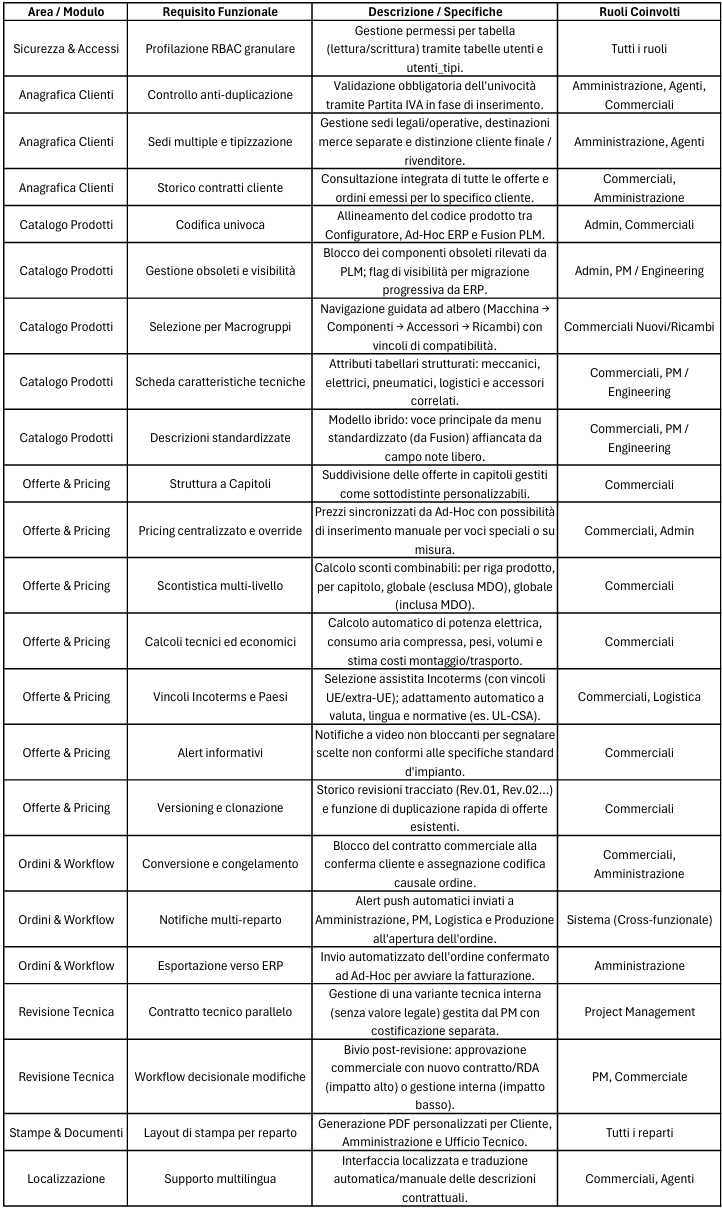
\includegraphics[width=0.8\linewidth]{Tabelle/RequisitiFunzionali.png}
    \caption{Requisiti funzionali raccolti.}\label{tab:RequisitiFunzionali}
\end{table}
\section{Requisiti non funzionali}
Questa sezione, a differenza della precedente, raccoglie i requisiti non funzionali.
In linea di massima, i requisiti non funzionali mirano
a migliorare l'attuale esperienza utente.
Sono da attenzionare in particolare la fluidità del sistema,
l'intuitività delle interfacce, e la velocità di esecuzione.
Le interfacce devono essere predisposte per device mobili e
proporre all'utente solo ciò che il suo ruolo necessita.
Tra i requisiti non funzionali, è emerso come sia necessario gestire la
raccolta dei dati da altri database, anche a runtime, per garantire la correttezza dei dati e la loro integrità.
Un esempio sono le giacenze dei prodotti in magazzino.
La tabella~\ref{tab:RequisitiNonFunzionali} seguente,
insieme al requisito stesso, raccoglie anche la sua categoria
e la sua priorità all'interno dell'implementazione.
I requisiti sono ordinati per priorità.
\begin{table}[H]
    \centering
    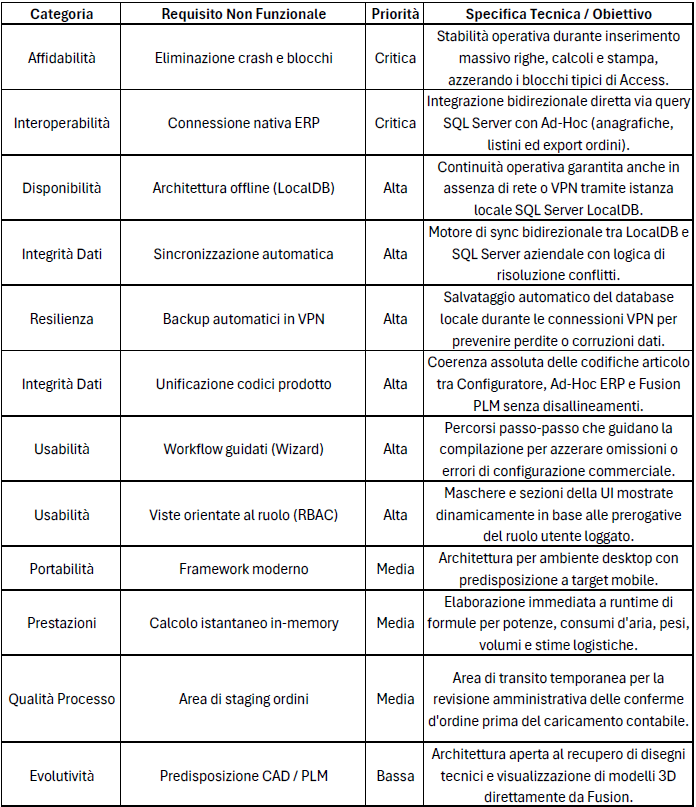
\includegraphics[width=0.9\linewidth]{Tabelle/RequisitiNonFunzionali.png}
    \caption{Requisiti non funzionali raccolti.}\label{tab:RequisitiNonFunzionali}
\end{table}

\section{Flussi di lavoro}
I flussi di lavoro citati in figura~\ref{fig:Flusso di un contratto} sono risultati complessi e poco efficienti.
Si è quindi deciso di inserire una revisione tecnica, da parte di un utente specializzato,
degli impianti venduti.
Il nuovo diagramma, in figura~\ref{fig:Nuovo diagramma degli stati di un contratto.}, mostra
un flusso più lineare che porta a valle meno errori.
Determinare i nuovi flussi lavorativi è fondamentale per progettare gli automatismi
a cui sono soggette le notifiche intra-reparto.
\begin{figure}[H]
    \centering
    \fbox{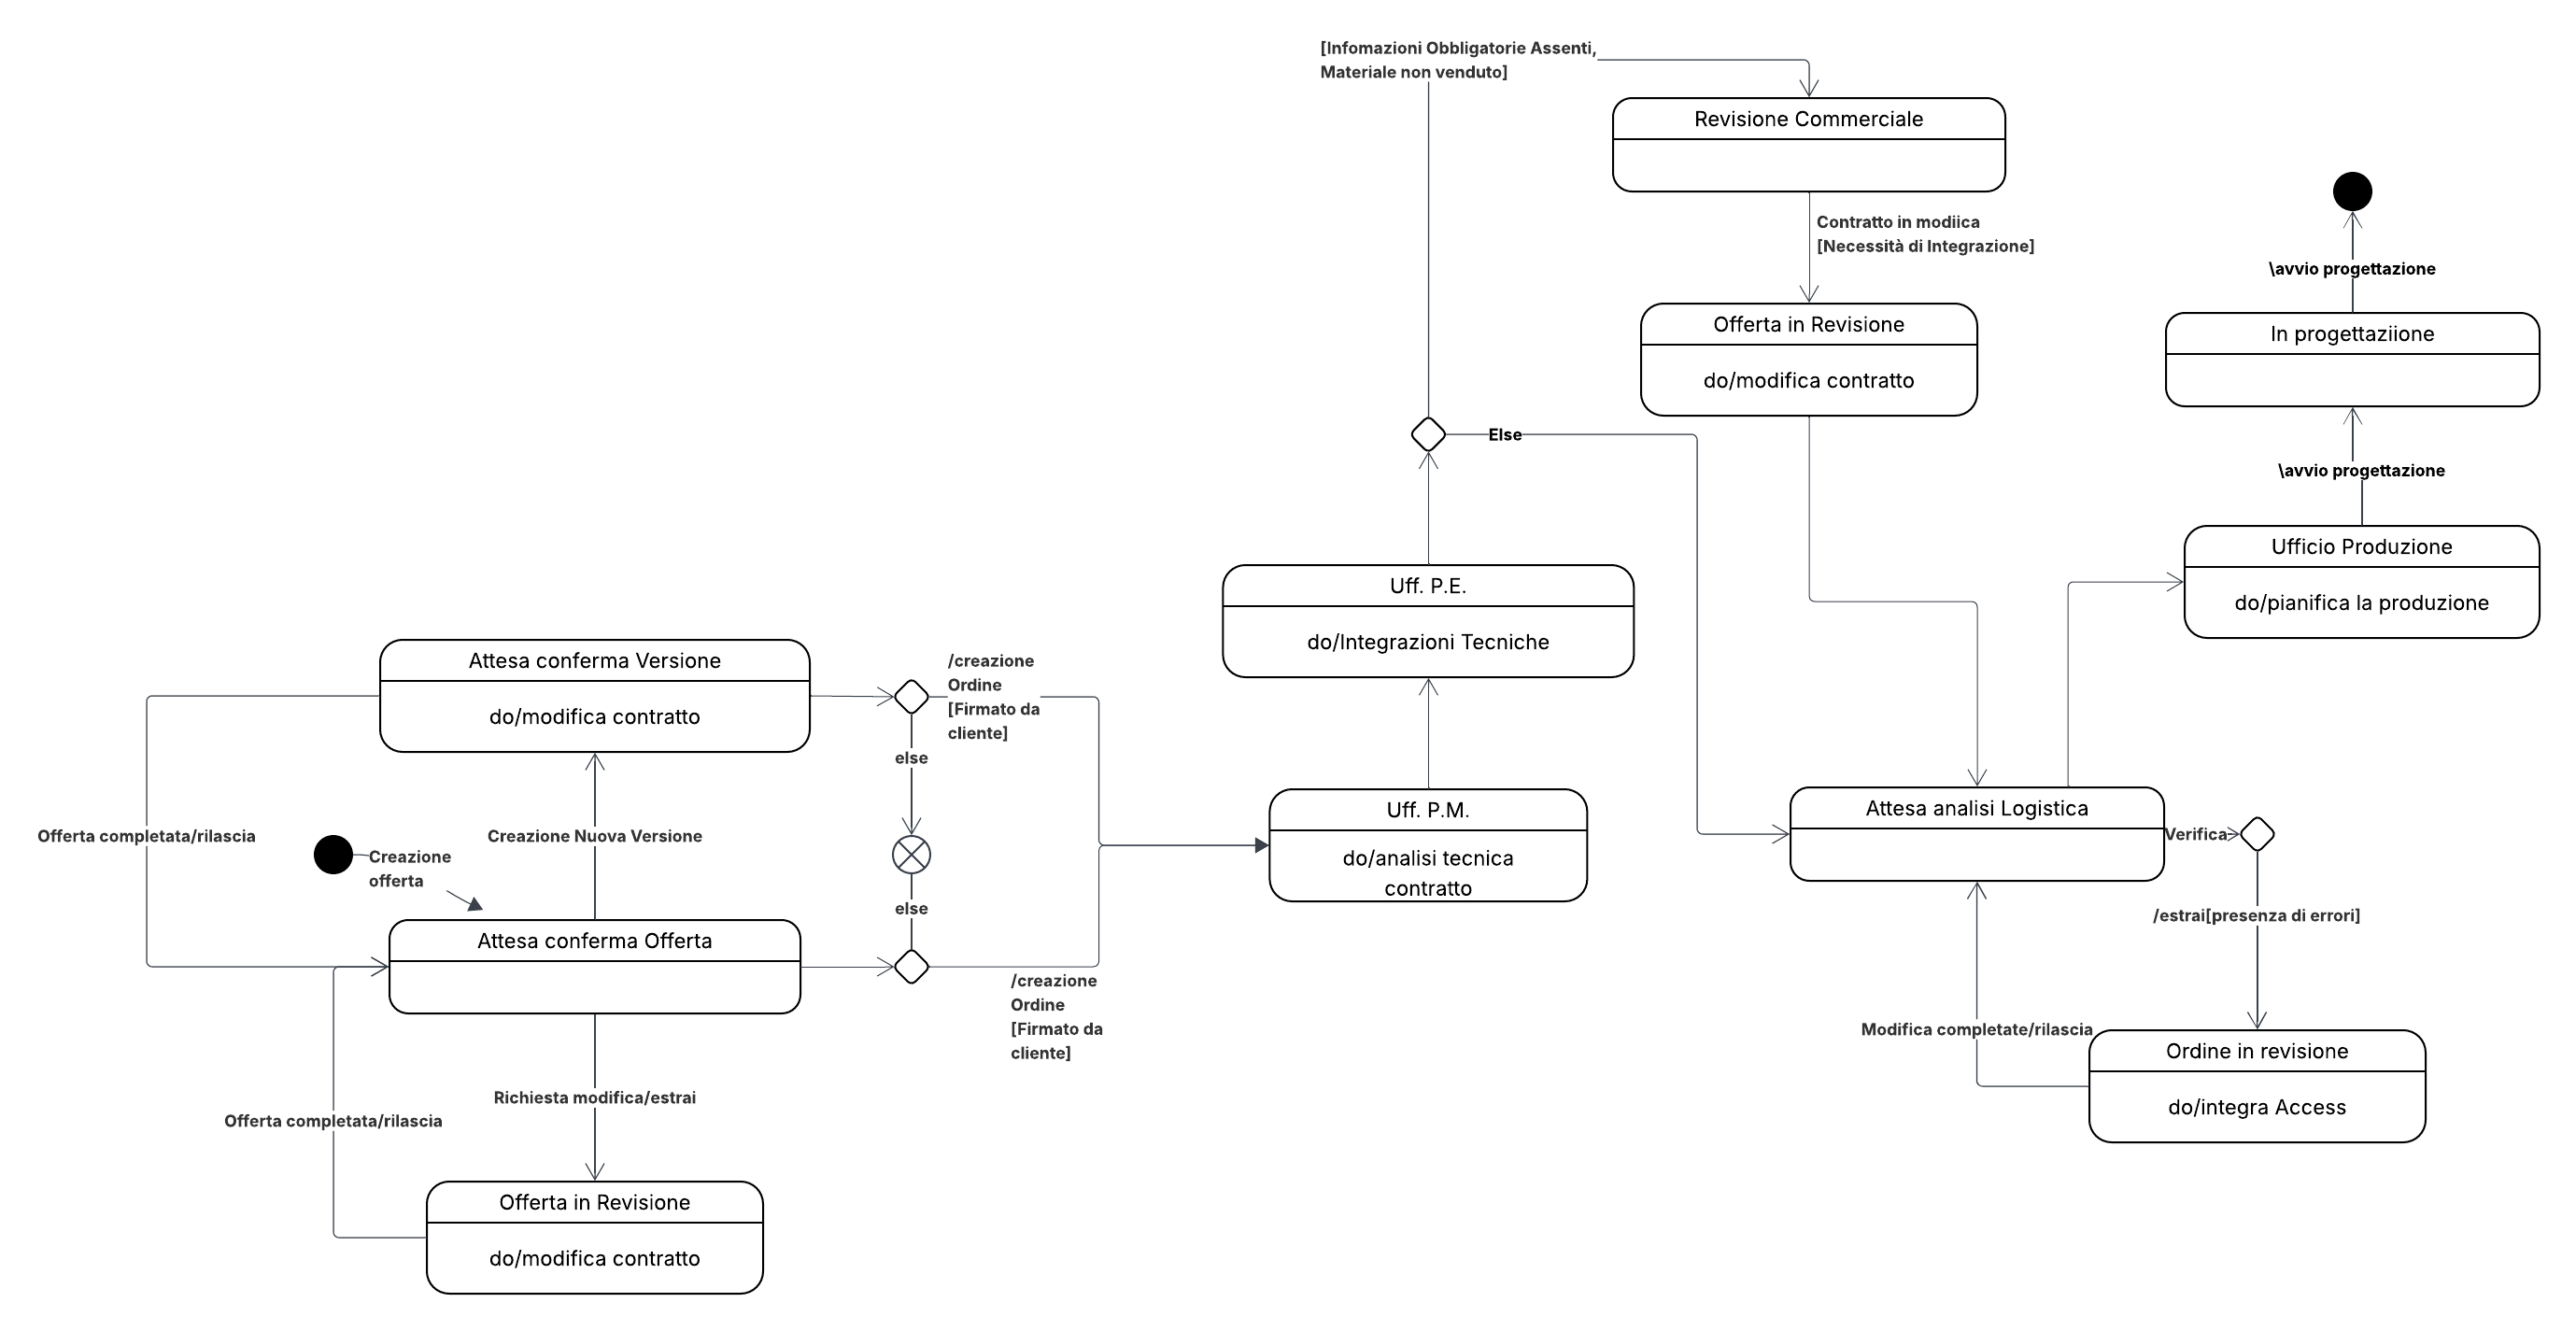
\includegraphics[width=1\linewidth]{figures/New Order flow.png}}
    \caption{Nuovo diagramma degli stati di un contratto}\label{fig:Nuovo diagramma degli stati di un contratto.}
\end{figure}

\chapter{Progettazione dell'architettura}\label{chapter:architettura}
\section{Premessa sulle scelte architetturali}
Le scelte architetturali sono dipese in primo luogo dall'infrastruttura aziendale,
e successivamente dalle richieste degli utenti durante gli incontri.
L'utilizzo di \sqlserver{}, come motore di database, è stato adottato come base di tutte le scelte successive.
Tale decisione è stata presa in quanto esso è già presente in azienda, pertanto non richiede ulteriori investimenti.
Un'ulteriore motivazione è che tale motore contiene i dati dell' \ac{ERP} aziendale e del \ac{PLM} di prodotto.
Mantenendo lo stesso motore di database, si è potuto garantire la compatibilità dei dati e la loro integrità.
Da questo caposaldo, la ricerca si è indirizzata verso un framework che interagisse
sia con \sqlserver{} sia con SQLite.\cite{SQLite}.
La necessità di operare offline ha guidato la ricerca di un sistema installabile in locale,
escludendo così le soluzioni web based.
La scelta è quindi ricaduta sulla piattaforma \dotnet\cite{DotNet} con il linguaggio
\csharp{} che, in quanto parte dell'ecosistema Microsoft,
è perfettamente integrata con i database prima citati.
La piattaforma \dotnet{} è espandibile mediante l'utilizzo di \nuget{}\cite{NuGet},
che permette di aggiungere package e quindi funzionalità al progetto.
I pacchetti sono sviluppati sia da Microsoft sia da terze parti,
e vengono aggiornati e supportati continuamente.
Questa manutenzione continua evita di incorrere in debiti tecnici futuri.
L'ambiente \dotnet{} è nativamente multipiattaforma
e questa proprietà soddisfa le necessità dei richiedenti.
Secondo le linee guida Microsoft, per lo sviluppo delle view multipiattaforma,
è consigliato l'utilizzo del package \nuget{} \dotnet{} \maui{}\cite{MAUI}.
In fase di compilazione, \maui{} converte il codice sorgente in codice nativo per la piattaforma di destinazione.
\maui{}, integrato con il package \nuget{} ``Community Toolkit Maui''\cite{ComTolkit}, consente
di costruire le interfacce grafiche in codice \csharp.
Nativamente \maui{} supporta solo il linguaggio Markup \xaml\cite{XAML}.

\section{Deployment}
La scelta degli ambienti di sviluppo precedentemente citati porta
a dover considerare il deployment dell'applicativo.
Il software verrà installato in locale su ogni dispositivo, sia esso desktop o mobile,
e si connetterà al database centrale.
All'interno dell'azienda è presente un dominio \ac{AD}, dove ogni oggetto del
dominio ha un \ac{IP} statico.
Questa configurazione permette la connessione al database, risiedente in un server all'interno del dominio,
in modo agile tramite \ac{IP}, se si è connessi all'interno della \ac{LAN}.
Lo scambio di dati tra il frontend e il backend avviene mediante protocollo \ac{TCP/IP}.
Si è valutato, per chi accede dall'esterno del dominio, di utilizzare la rete \ac{VPN},
stabilendo una connessione virtuale che permette di essere all'interno della \ac{LAN}.
Il database locale, in SQLite, è strutturato come una copia del database centrale.
I dati vengono allineati tra i due database mediante un processo di sincronizzazione.
In assenza di connessione, verificabile tramite ping, si accede al database locale e
una volta ristabilita la connessione, i dati vengono sincronizzati.
Il diagramma dei deployment è riassunto in figura~\ref{fig:Diagramma dei deployment}.
\begin{figure}[H]
    \centering
    \fbox{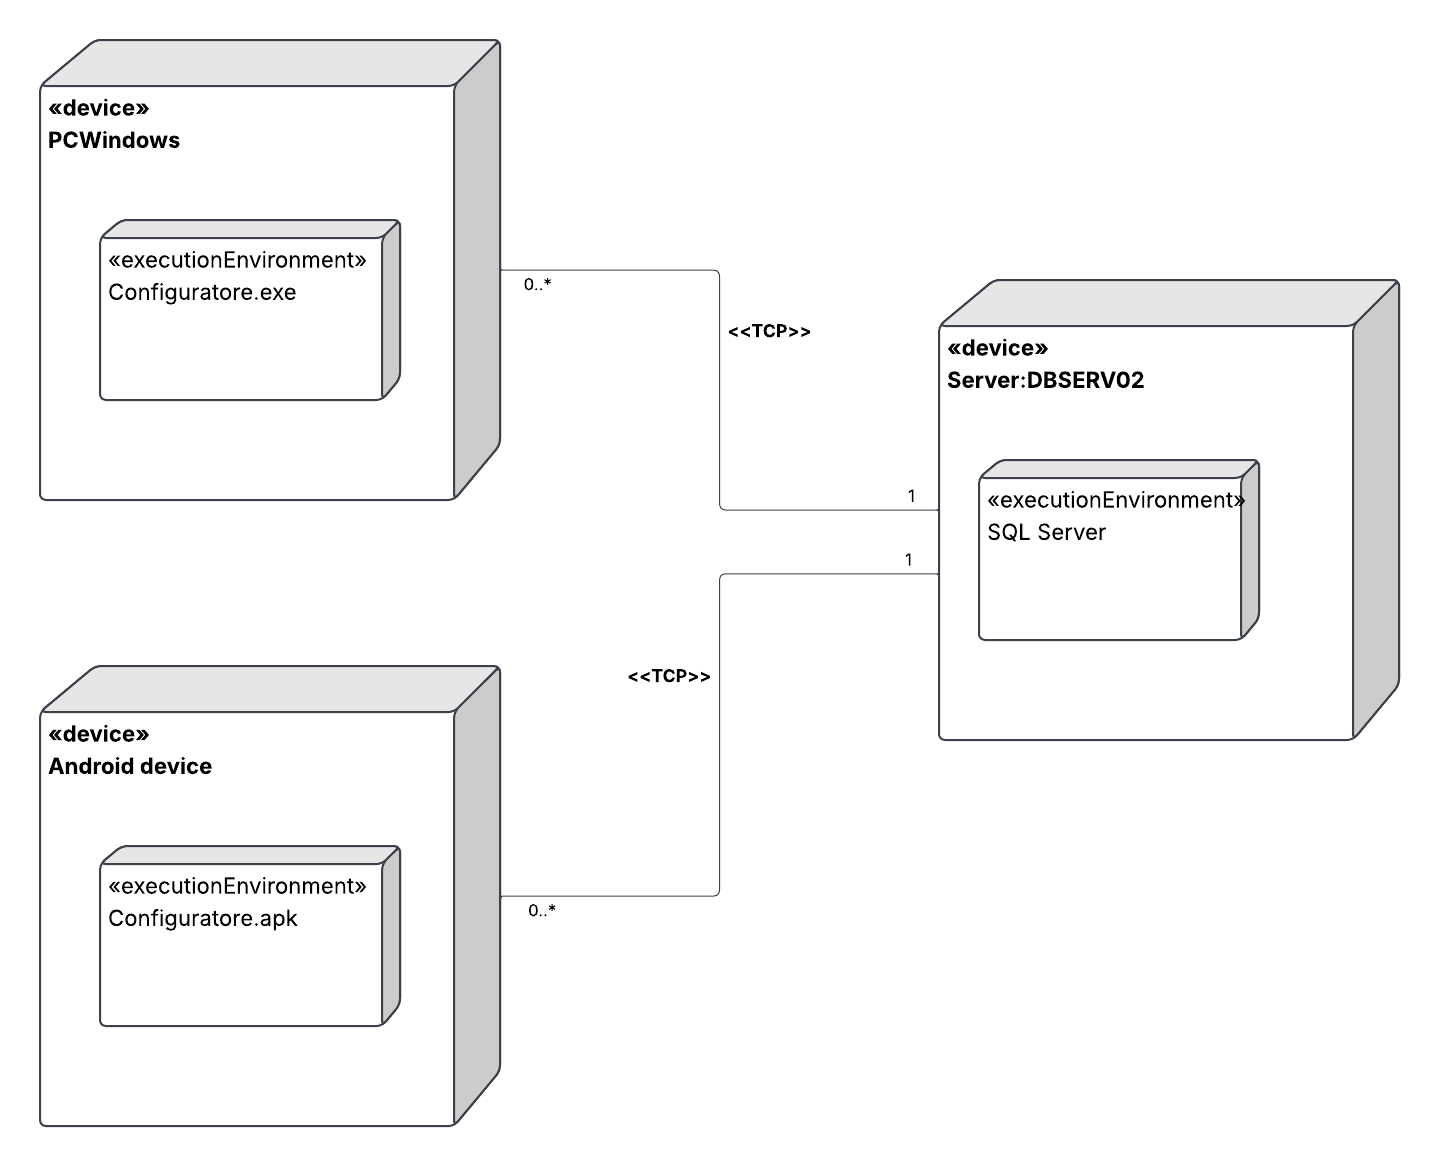
\includegraphics[width=1\linewidth]{figures/Deployment.png}}
    \caption{Diagramma dei deployment}\label{fig:Diagramma dei deployment}
\end{figure}
Nella fase di sviluppo, per testare la struttura del database,
è stato scelto di utilizzare una versione di \sqlserver{} locale, denominata SQL Express~\cite{SQLExpress}.
SQL Express condivide con \sqlserver{} tutte le caratteristiche principali.
Questa proprietà ha permesso di costruire query e testare funzionalità localmente in modo compatibile
con il database di produzione.

\section{Package}
L'intero software è stato suddiviso in tre distinti package, con responsabilità diverse.
Si è cercato di seguire il principio \ac{DRY} e la riusabilità degli stessi.
Il principio \ac{DRY} consiste nel non ripetere il codice già scritto, ma nel riutilizzarlo.
Questo approccio permette di ridurre la complessità del software, facilitando la manutenzione e l'evoluzione futura.
Il mantenimento del principio \ac{DRY} necessita di continua rifattorizzazione del codice.

\subsection{Interfaccia al database}
Il package di interfaccia al database, denominato ``DatabaseManagementPackage'',
ha il compito di gestire tutti gli aspetti legati a quest'ultimo, come:
\begin{itemize}
    \item gestione delle connessioni ai vari database, come \sqlite{} e \sqlserver{} o nel caso dei test, SQL Express;
    \item gestione delle transazioni;
    \item gestione dei permessi utente, bloccando le operazioni non consentite;
    \item conversione, mediante \ac{ORM}, delle tabelle del database in entity;
    \item mappatura di entity in file neutri, proteggendo il database;
    \item gestione di Repository per ogni entità, che espongono le operazioni \ac{CRUD};
    \item gestione di una suite di test per verificare le operazioni precedenti.
          Questa suite è risultata fondamentale nell'evoluzione del database,
          validando i cambiamenti apportati;
    \item esposizione al di fuori del package di soli file neutri e della classe manager del database.
\end{itemize}
Nell'implementazione si è utilizzato il pacchetto \nuget{} \ac{EF Core}~\cite{EFCore}.
Questo modulo permette una gestione efficiente delle operazioni di accesso ai dati,
consentendo di astrarre le tabelle del database in classi di entity.
Le entity sono state a loro volta mappate in \ac{DTO}.
Un \ac{DTO} è un design pattern architetturale ideato
per ottimizzare lo scambio di informazioni tra diversi layer di un'applicazione.
Opera come un aggregatore leggero che raggruppa i dati necessari
per una specifica comunicazione (come il traffico client-server).
Privo di logica di business o comportamenti applicativi, il \ac{DTO}
espone esclusivamente le proprietà richieste dal caso d'uso:
questa semplificazione minimizza la dimensione del payload,
riduce le chiamate di rete e la latenza complessiva, ottimizzando le prestazioni del sistema.
La traduzione da entity a \ac{DTO} protegge i dati del database, evitando che vengano esposti direttamente\cite{DTO}.
Questa seconda mappatura è stata realizzata mediante il package ``Mapster''~\cite{Mapster},
appartenente a terze parti.
La mappatura entity-\ac{DTO} è stata realizzata in modo bidirezionale in quanto, in alcuni casi,
è necessario convertire un \ac{DTO} in entity per poterlo salvare nel database.

\subsection{Libreria di componenti view}
La creazione di interfacce grafiche è stata supportata da un package dedicato,
che racchiude in sé factory di componenti, costanti e utilità.
Il package, denominato ``ViewComponentLibrary'', è stato concepito a sé stante
per favorire un suo impiego in implementazioni future.
La libreria si appoggia a sua volta al package \nuget{} ``Community Toolkit Maui''\cite{ComTolkit}.
Questo package permette di scrivere le interfacce grafiche in codice \csharp{} Markup,
evitando quindi l'utilizzo del linguaggio \xaml\cite{XAML},
standard di sviluppo per le interfacce MAUI.\

\subsection{Modulo main e view}
Il package principale del progetto è dedicato alla gestione dei componenti
e dei flussi di lavoro.
Il package, denominato ``ConfiguratoreCommerciale'', ha numerosi compiti,
tra cui la gestione della Dependency Injection, la creazione delle view e dei rispettivi ViewModel.
In questo package risiedono infatti i ViewModel, che si interpongono tra le view e i repository,
esponendo i dati tramite proprietà osservabili (Observable Properties).
La Dependency Injection, invece, permette di iniettare
le dipendenze necessarie alle classi, come ad esempio i repository, le classi di logging o le view stesse se registrate.
Le classi di view, utilizzando i componenti della libreria,
vengono realizzate tenendo conto del dispositivo di destinazione.
La differenziazione è permessa dall'utilizzo della compilazione condizionale,
distinguendo il codice da compilare in base alla piattaforma di destinazione.
Un esempio di tale condizione è il seguente:
\begin{lstlisting}[language=CSharp]
#if ANDROID
    // codice per piattaforma Android
#elif WINDOWS
    // codice per piattaforma Windows
#endif
\end{lstlisting}
Questa possibilità permette anche di eseguire parti di codice solo in fase di DEBUG.\
Gli aspetti generali gestiti dal package possono essere riassunti come segue:
\begin{itemize}
    \item creazione delle interfacce grafiche;
    \item traduzione a compile time del codice \csharp{} in \xaml{};
    \item traduzione a compile time in elementi nativi per la piattaforma di destinazione;
    \item gestione delle interfacce mediante ViewModel,
          che a loro volta tramite proprietà osservabili modificano la view in risposta ad eventi;
    \item gestione della navigazione tra le interfacce grafiche;
    \item gestione dei permessi, mostrando solo i comandi che competono al ruolo dell'utente;
    \item gestione della Dependency Injection mediante la classe \textit{MauiProgram.cs};
    \item creazione, in fase di avvio, di una cache in \ac{RAM}
          di dati immutabili durante la sessione, come tabelle di lookup.
\end{itemize}
Il diagramma dei package è riassunto in figura~\ref{fig:Diagramma dei package}.
\begin{figure}[H]
    \centering
    \fbox{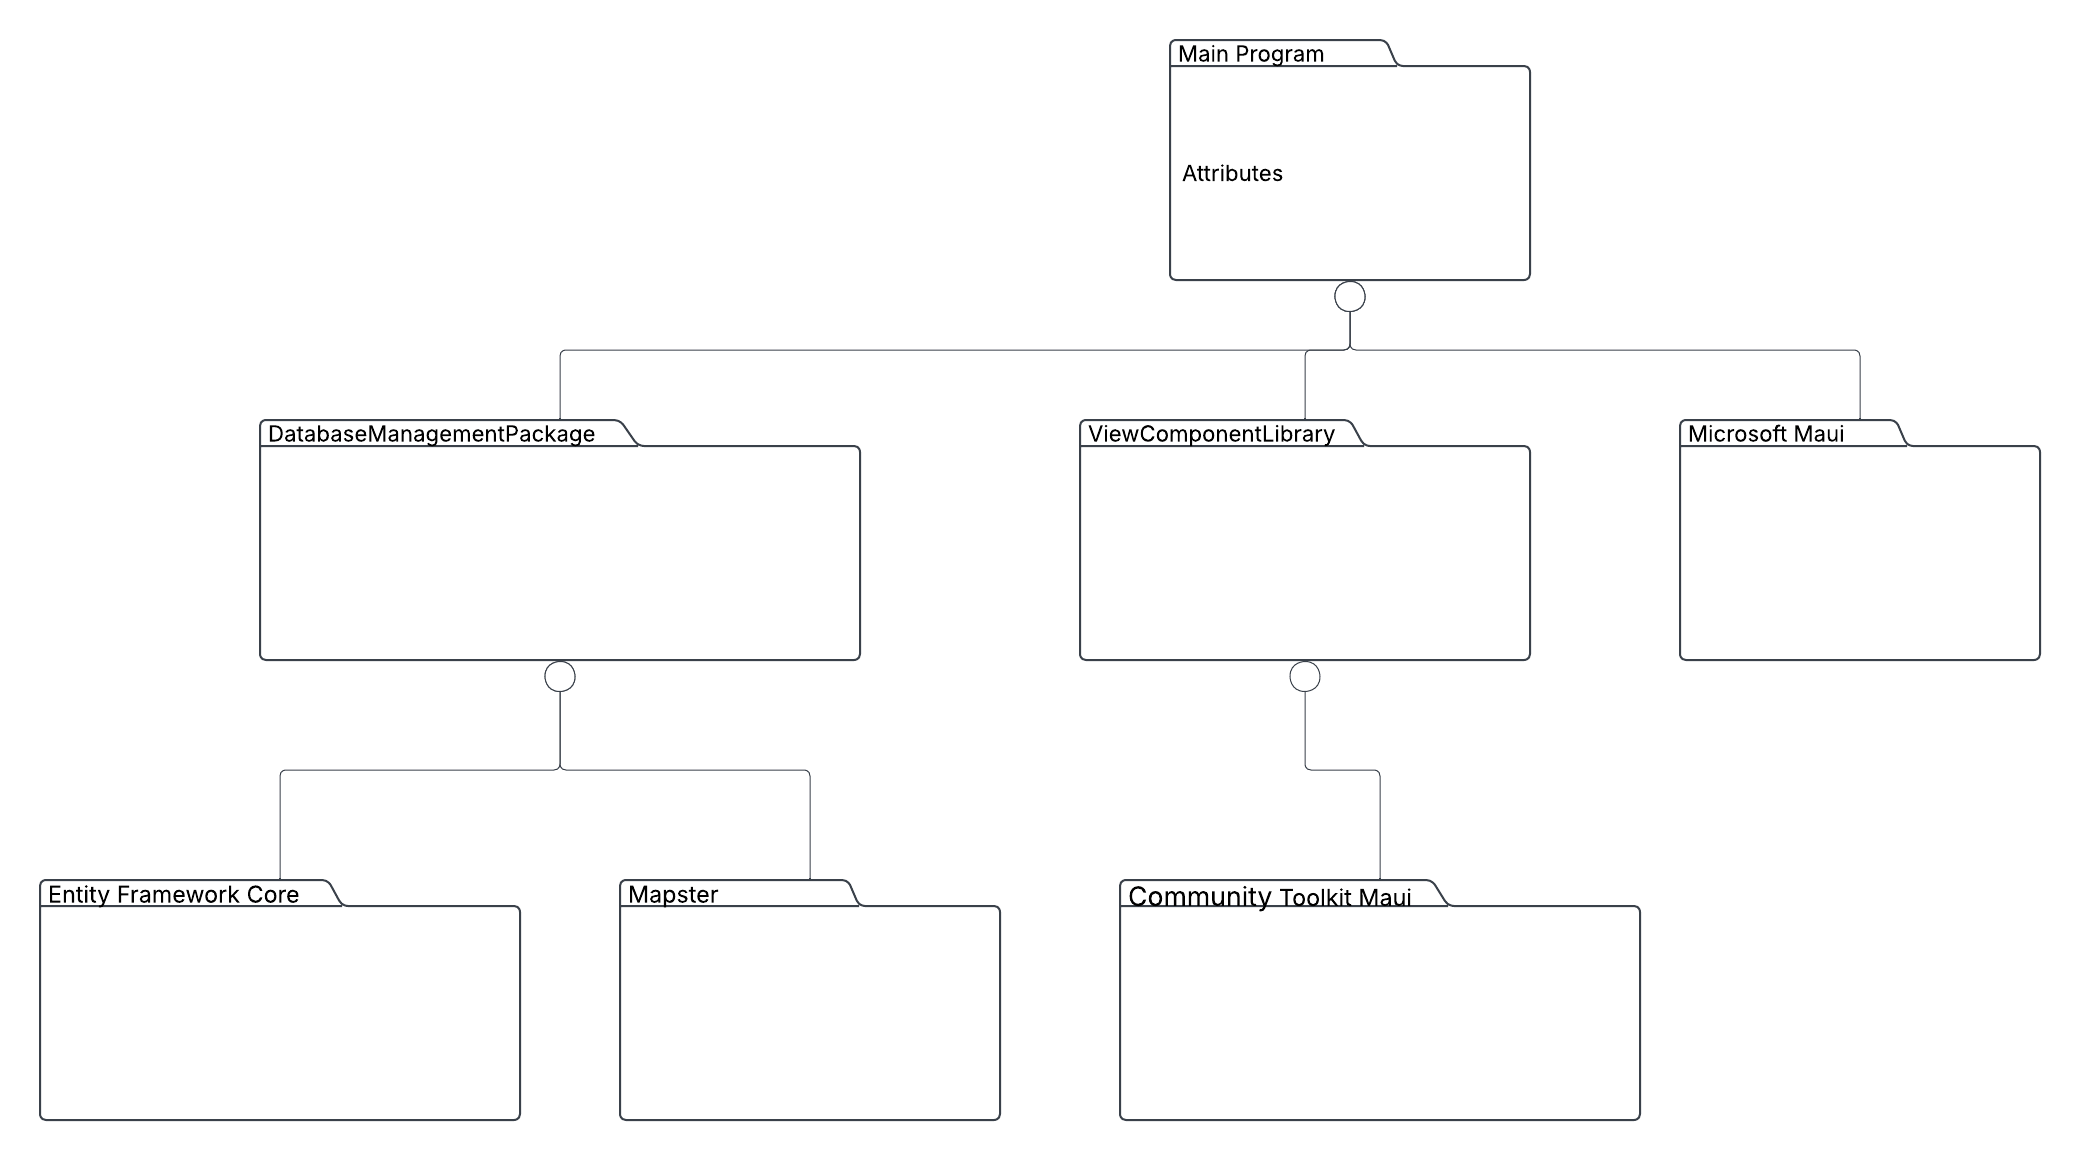
\includegraphics[width=1\linewidth]{figures/DiagramnaPackage.png}}
    \caption{Diagramma dei package}\label{fig:Diagramma dei package}
\end{figure}

\chapter{Scelte progettuali}\label{chap:ScelteProgettuali}
\section{Scelta modello di sviluppo}
Il modello di sviluppo scelto è basato sulla necessità di prototipare e testare
con gli utenti le funzioni nell'arco dell'intero sviluppo.
Si è quindi deciso di adottare un modello agile,
supportato dalla creazione di test delle funzioni e dei prototipi delle interfacce.
La progettazione è stata iterativa e incrementale, seguendo i canoni dell'agilità.
Tutti i metodi di interazione col database sono stati testati da appositi Unit Test
che ne validassero il comportamento.
I test di regressione hanno permesso di convalidare le modifiche apportate al database e di
conseguenza al software.
Le interfacce grafiche, al contrario, non sono state supportate da test, ma prototipate e
approvate da utenti scelti.
La rifattorizzazione del codice è stata affrontata con regolarità seguendo il principio \ac{DRY}.
Nel seguire tale principio, si sono create più classi di Factory e classi di utilità
che unificassero quanto più possibile il codice comune.

\section{Suddivisione e contenuto dei rilasci}
Le tempistiche dei rilasci sono state
decise insieme al Project Manager aziendale.
Il collega è stato di supporto nella stima dei tempi di sviluppo e nella
conversione del database esistente, guidando lo sviluppo attraverso le tecniche professionali.
Nel primo rilascio, si è scelto di includere tutti i requisiti già
presenti nel precedente applicativo.
In tale rilascio, con consegna stimata per gennaio 2027, sono presenti le
seguenti funzionalità:
\begin{itemize}
    \item gestione utenti e permessi;
    \item anagrafica clienti;
    \item creazione delle offerte;
    \item versioning offerte;
    \item creazione ordini;
    \item import ed export dati, da e verso altri database;
    \item creazione reportistica;
    \item gestione multilingua dell'interfaccia applicativa;
    \item prototipo mobile;
    \item modulo di configurazione prodotto.
\end{itemize}
Si è scelto di non includere la funzionalità offline,
in quanto essa necessita di un database centrale stabile.
La funzionalità offline verrà implementata nel secondo rilascio.
Questa fase avverrà una volta che il software sarà in produzione, per poter contare su un database pressoché stabile.
Nel secondo rilascio saranno quindi presenti:
\begin{itemize}
    \item gestione revisione tecnica e differenze con contratto firmato;
    \item inserimento di calcoli automatici sulla base delle caratteristiche del venduto (es.\ potenza elettrica totale assorbita);
    \item gestione multi-valuta per ordini internazionali;
    \item apertura dei disegni \pdf{} dal server del \ac{PLM};
    \item report avanzati;
    \item implementazione database locale con logiche di sincronizzazione.
\end{itemize}

\section{Scelta framework ORM}
All'interno della sezione sull'architettura, è stata citata la scelta del framework \ac{EF Core}.
Questo framework ha permesso di mappare le tabelle del database in classi mediante la tecnica \ac{ORM}.
La tecnica \ac{ORM} permette di gestire il database con un approccio \ac{OOP}, astraendo le tabelle in classi.
Le mappature relazionali a oggetti \ac{ORM} collegano le applicazioni scritte in un linguaggio di programmazione
\ac{OOP} ad un database sottostante.
Questi tipi di applicazioni e database vengono spesso utilizzati insieme,
ma ognuno gestisce i dati in modo diverso. L’aggiunta di una mappatura relazionale
a oggetti consente a ciascuno di inviare dati in un formato comprensibile all’altro.
È possibile modificarne uno senza influire sull’altro.~\cite{ORM}
I legami tra le entità sono gestiti mediante la classe \texttt{Context}.
L'\ac{ORM} ha permesso, con l'utilizzo di script PowerShell,
di ricreare in modo rapido tutte le entity e il context a fronte di cambiamenti del database.
Tale approccio può essere definito database-first, in quanto la progettazione avviene principalmente sul database
e il software ne eredita le modifiche.
Le query sono state scritte tramite le funzioni \ac{LINQ}, che hanno permesso di formularle in linguaggio \csharp{}.
Un esempio di query è riportato nella funzione~\ref{lst:esempio-query-linq}.
\lstinputlisting[
    language=CSharp,
    caption={Esempio di query LINQ},
    label={lst:esempio-query-linq}
]{listings/LINQ-example.cs}

In ottica di offline, le query in \ac{LINQ} sono compatibili con il database locale \sqlite{} se si limitano
le funzioni utilizzate a quelle supportate da esso.
Le funzioni compatibili sono ad esempio: \textit{Where, Select, OrderBy, GroupBy, Join, Distinct}.

Uno degli aspetti negativi di \ac{LINQ} è la lentezza con grandi volumi di dati.
Lo svantaggio è dovuto alla traduzione del codice in query compatibili con \ac{SQL}.
Si è valutato però, in caso si presentino problemi di performance,
di ottimizzare il database mediante indici in prima battuta
e, successivamente, ottimizzando le singole query.
\ac{EF Core} permette di ottimizzare le query scrivendole in \ac{SQL} puro,
bypassando la traduzione da \ac{LINQ}.

\section{Scelta del framework grafico}
Il framework grafico scelto aveva come obiettivo soddisfare il requisito della portabilità e dell'offline.
Le scelte vagliate sono state:
\begin{itemize}
    \item frontend web based, con l'utilizzo di \ac{HTML}, \ac{CSS} e \ac{JS} e interrogazione
          del database centrale mediante \ac{API};
    \item utilizzo del framework \maui{}, nativamente cross-platform e integrato perfettamente con il backend.
\end{itemize}
L'opzione web based, con interfacce facilmente adattabili a qualsiasi dispositivo,
ha presentato due svantaggi principali.
La difficoltà principale risiedeva nell'utilizzo in assenza di connessione.
In questo scenario, per funzionare, richiedeva che i file e il database fossero presenti sul dispositivo.
Questa caratteristica rende difficoltoso gestire gli aggiornamenti.
Il secondo motivo, non trascurabile per le tempistiche,
è l'utilizzo di più linguaggi di programmazione.
Quest'ultimo non massimizza l'esperienza acquisita con l'implementazione degli altri moduli.
Il framework \maui{} di \dotnet{} sopperisce a entrambi i problemi.
Il programma è fisicamente installato sui dispositivi e il loro aggiornamento
può essere gestito centralmente all'interno di uno store Microsoft.
Essendo basato su \dotnet{} e avvalendosi del framework ``Community Toolkit Maui'',
le interfacce sono scritte in \csharp.

\section{Scelta del pattern di progettazione}
Insieme a \maui{}, Microsoft suggerisce l'utilizzo del pattern \ac{MVVM}\cite{MVVM}.
Il modello \ac{MVVM} consente di separare in modo pulito le logiche
di business e le relative interfacce utente.
La gestione separata risolve numerosi problemi, quali la possibilità di ridisegnare
le interfacce utente senza dover modificare le classi che le governano.
Un secondo vantaggio è la possibilità di consentire agli sviluppatori e
ai progettisti dell'interfaccia utente di collaborare
più facilmente durante lo sviluppo delle rispettive parti di un'app\cite{MVVM}.
Il modello \ac{MVVM} è composto da tre elementi fondamentali che interagiscono
come in figura~\ref{fig:Diagramma funzionamento MVVM}:
\begin{figure}[H]
    \centering
    \fbox{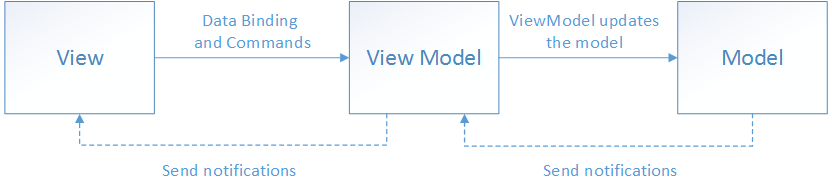
\includegraphics[width=1\linewidth]{figures/mvvm-pattern.png}}
    \caption{Diagramma funzionamento MVVM}\label{fig:Diagramma funzionamento MVVM}
\end{figure}
Questo modello, separando la logica della view da quella di business,
ha permesso di prototipare le interfacce nei primi rilasci e in futuro riprogettarle
migliorando l'accessibilità, ovvero la capacità di un prodotto di essere utilizzato da persone con disabilità.
Migliorarla vuol dire aggiungere valore e rimuovere le barriere che potrebbero impedire l'interazione con esso.
Un altro aspetto migliorabile è l'\ac{UX}, ovvero l'esperienza dell'utente nell'interazione con il prodotto.

\chapter{Progettazione del database}\label{chap:Database}
\section{Esportazione vecchio database}
La creazione della nuova base di dati è partita dall'esportazione e dallo studio dell'attuale database Access.
L'esportazione è avvenuta per mezzo di \ac{SSMA},
che ha permesso di esportare solo la struttura esistente da Access in \sqlserver{}.
\ac{SSMA} è uno strumento progettato per automatizzare la migrazione del database a \sqlserver{},
da Microsoft Access, Db2, MySQL, Oracle e SAP ASE.~\cite{SQLServerMigrationAssistant}
Ottenuta l'attuale struttura, essa ha subito un processo di ristrutturazione
che ha portato ad avere un database più leggibile, manutenibile e performante.
\section{Denominazione tabelle e campi}
Il primo intervento effettuato è stato quello di rinominare le tabelle ed i campi del database.
Le modifiche addottate sono state le seguenti:
\begin{itemize}
    \item Denominare le tabelle in minuscolo, separati da underscore, ad esempio: \textit{nome\_tabella}.
    \item Denominare i campi delle tabelle in minuscolo, separati da underscore,con
          il prefisso della tabella per renderlo univoco. Un esempio di campo è: \textit{prefTabella\_nomeCampo}.
    \item Le chiavi primarie di ogni tabella sono degli indici progressivi, rendendo unica ogni riga.
          Il campo segue il pattern \textit{prefTabella\_id}.
\end{itemize}
Insieme alle modifiche sopra citate, sono stati aggiunti dei campi di audit,
come data ed utente di creazione, ma anche data e utente di modifica.
Queste informazioni permettono di avere un tracciamento delle modifiche e di chi le ha effettuate.
Un ulteriore campo comune aggiunto è \textit{deleted},
booleano per la gestione della cancellazione logica.
Si è deciso di non cancellare mai fisicamente i dati, ma di marcare le righe come cancellate
per facilitare il ripristino dei dati in caso di errore.
Questi campi trasversali sono fondamentali per la gestione dei dati
e la manutenzione del database.
\section{Utilizzo di SSIS nel processo di migrazione}
I successivi processi di modifica e popolamento del database sono stati gestiti tramite
\ac{SSIS}.~\cite{SQLServerIntegration}
Questo strumento permette la creazione e l'esecuzione di pacchetti di query,
che possono essere schedulati o eseguiti manualmente.
Mediante interfaccia grafica è possibile creare flussi di query, con l'opportunità di gestire
eccezioni, condizioni di esecuzione e logiche di flusso.
Il principale utilizzo di \ac{SSIS} è stato quello di organizzare
un flusso di query per la creazione e popolamento del database.
Il primo flusso gestito è il seguente:
\begin{enumerate}
    \item crea se non esiste il database;
    \item se presenti le tabelle, le elimina;
    \item crea le tabelle seguendo un ordine consono alle foreign key;
    \item popola le tabelle di lookup;
    \item popola le tabelle con dati del vecchio database;
    \item popola le tabelle restanti con dati di test.
\end{enumerate}
Tramite questo flusso è possibile creare un database pronto all'uso, con dati di test e dati reali,
ricostruito con facilità in caso di errori o modifiche.
Nelle fasi più avanzate, alle operazioni prima citate, sono state aggiunte
quelle per la creazione delle tabelle e dei trigger di backup, per la gestione dello storico dei dati.
A database quasi pronto, si è proceduto alla creazione di un secondo flusso di query per
l'importazione dei dati da altri database, come ad esempio \ac{ERP} e \ac{PLM}.
\section{Ristrutturazione database}
\subsection{Eliminazione ridondanze e normalizzazione}
La fase di studio dell'attuale database ha portato alla luce diverse ridondanze e dati non normalizzati.
All'interno erano presenti più tabelle con lo stesso contesto di utilizzo o tabelle non utilizzate.
Si è quindi proceduto all'eliminazione di tali tabelle ed alla normalizzazione delle restanti in \ac{2NF}.
La \ac{2NF} è una forma di normalizzazione delle tabelle del database,
che richiede che ogni attributo non chiave sia completamente dipendente dalla chiave primaria,
oltre che rispettare la \ac{1NF}.
La \ac{1NF} richiede che ogni attributo della tabella sia atomico, ovvero non divisibile in più parti.
Un'altra modifica sostanziale è stata l'unificazione di tabelle similari in un'unica tabella,
discriminate mediante campo \textit{prefTabella\_tipo} proveniente da un lookup dedicato.
Un esempio di questo contesto sono le tabelle di ``Offerta'' ed ``Ordine'',
dove una è la diretta evoluzione della precedente e mantengono gli stessi dati.
Le due tabelle sono state unite sotto il cappello della tabella ``Documenti'',
discriminata solo dal campo \textit{doc\_tipo}.
In queste tabelle, in particolare, era importante tenere traccia del legame Padre-Figlio.
È stato aggiunto un campo \textit{doc\_documento\_padre} che, mediante
chiave importata, permettesse di ricostruire il legame attraverso un auto join.
Il metodo così pensato, in ottica di ampliamento, permette la gestione di ulteriori
tipologie di documenti senza cambiare la struttura.
Un esempio è l'aggiunta della tipologia di documento ``Tecnico'',
che sarà l'evoluzione del documento ``Ordine'' e conterrà la revisione tecnica dell'ordine stesso.
\subsection{Creazione tabelle di lookup}
Come già prima accennato, le tabelle di lookup sono state create per discriminare le tipologie di dati.
Tali tabelle sono state pensate per garantire una estedibilità futura e far fronte a modifiche non previste.
Queste tabelle sono considerate fisse, e non possono essere modificate dall'utente finale,
ma solo da un amministratore tramite query.
Esse, con al più un campo descrittivo, rendono la gestione dei dati più semplice,
potendo filtrare le informazioni in base al loro tipo.
Un vantaggio, a livello di software, è il poterle mappare in classi di enumerazione,
rendendo il codice più leggibile ed evitando non necessari join nelle query.
Le classi di enumerazione sono una tipologia di classe che associa ad un insieme di costanti un valore.
Il vantaggio è quindi per ogni valore di lookup, avere un nome leggibile evitando di interrogare il database.
Un ultimo vantaggio, essendo appunto fisse, è il poterle
caricare in memoria \ac{RAM} all'avvio dell'applicativo, evitando di interrogare il database ad ogni richiesta.

\subsection{Aggiunta tabelle non presenti}
\subsubsection{Gestione dei prodotti}
Il database originale utilizzava i prodotti come oggetti atomici, senza la possibilità di gestire i loro componenti.
Si è quindi deciso di creare le distinte prodotto. La tabella \textit{Prodotti} è stata messa in auto
join con cardinalità N:M.
Tale relazione a livello di schema logico è stata realizzata mediante la tabella \textit{Prodotti\_composizioni}.
La tabella in questione aggiunge, oltre alle chiavi
dei prodotti, anche il quantitativo della riga stessa e la posizione di apparizione.
Lo schema ER risultante è visibile in figura~\ref{fig:ERProdotti}, mentre lo schema logico 
è visibile in figura~\ref{fig:LOGProdotti}.
        \begin{figure}[H]
            \centering
            \fbox{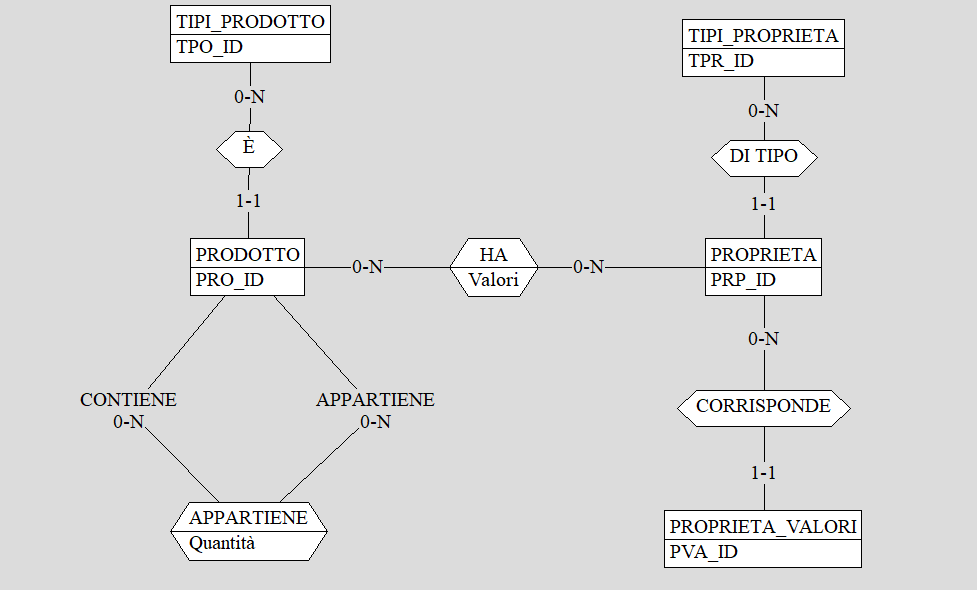
\includegraphics[width=1\linewidth]{figures/ER_PRODOTTI.png}}
            \caption{Schema \ac{ER} dei prodotti}\label{fig:ERProdotti}
        \end{figure}
    \begin{figure}[H]
        \centering
        \fbox{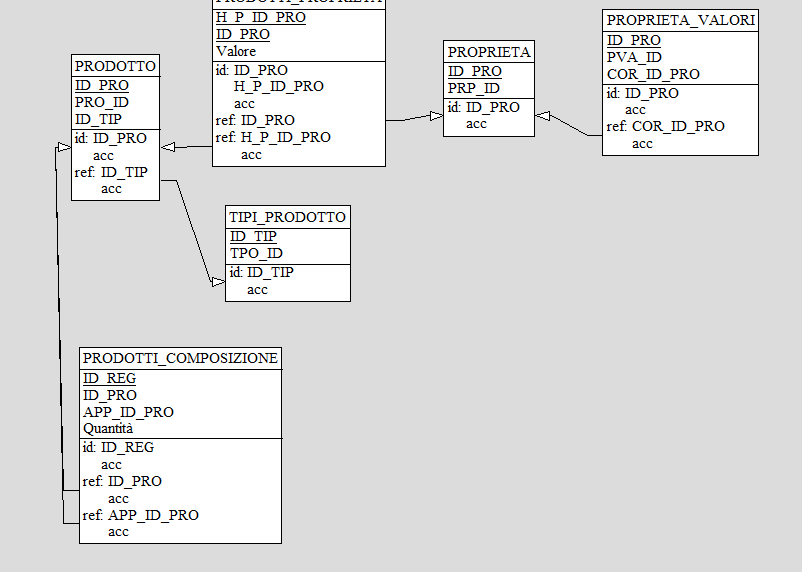
\includegraphics[width=1\linewidth]{figures/Logico_PRODOTTI.png}}
        \caption{Schema logico dei prodotti}\label{fig:LOGProdotti}
    \end{figure}
La tabella prodotti, ovvero i compoenenti base o aggregati, sono posti in auto join con se stessi.
La relazione così composta permette di gestire multilivelli di profondità.
Ad ogni prodotto sono associate N proprietà, ed a sua volta, ad ogni proprietà sono associati N prodotti.
La relazione che li lega raccoglie inoltre un valore dedicato del valore della proprietà.
La tabella proprità\_valori messa in associazione 1:N con la tabella della proprietà, raccoglie i valori standard assegnabili a tale proprietà.
I valori standard sono usati per compilira il campo Valore prima citato.
La tabella tipi\_proprietà permette di raggruppare le proprietà in base alla loro finalità.
Un esempio è la distinzione tra le proprietà meccaniche, elettriche e normative.

La gestione, così pensata, permette di effettuare ricerche approfondite.
Un esempio è quello della estrapolazione dei componenti di ricambio di un determinato prodotto, che possono
risiedere anche a più livelli di profondità.
Questo sistema, insieme ad appositi lookup, ha inoltre permesso la costruzione del modulo
``Configuratore'' per la configurazione di prodotto.~\ref{chapter:Configurazione}.
\subsubsection{Tabelle gestione lingue}
Si è deciso di aggiungere delle apposite tabelle per la gestione delle traduzioni di campi del database.
Le tabelle predisposte contengono al loro interno la chiave della tabella di riferimento,
il campo da tradurre e la chiave importata dalla tabella ``Lingue''.
Quest'ultima tabella non era presente nella soluzione di partenza.
La gestione così pensata permette di estendere le traduzioni a più lingue.
La gestione delle reportistiche dei documenti è gestita mediante una tabella dedicata.
Questa tabella mappa le tipologie di reportistica richieste dal cliente con le apposite lingue concordate.
Capita infatti di avere ad esempio manuali in lingua inglese, ma etichette sui macchinari con la lingua del luogo.
Il diagramma \ac{ER} delle lingue è visibile in figura~\ref{fig:ERLingue}.
%Aggiungere immagine
\begin{figure}[H]
    \centering
    \fbox{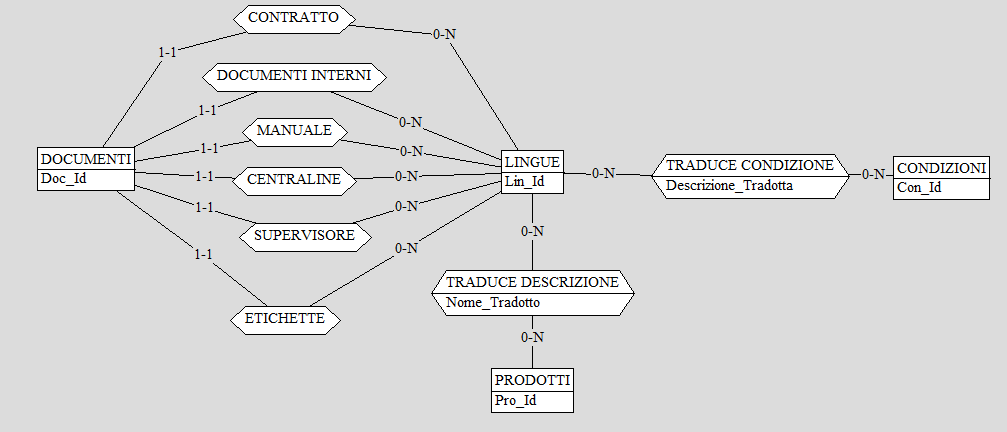
\includegraphics[width=1\linewidth]{figures/ER_LINGUE.png}}
    \caption{Schema \ac{ER} delle lingue}\label{fig:ERLingue}
\end{figure}
\subsubsection{Creazione tabelle di backup}
Si è scelto di gestire solo un ristretto numero di essenziali tabelle,
come ad esempio quelle dei documenti, dei prodotti, delle righe sia dei documenti che dei prodotti.
La gestione non è stata capillare su tutte le tabelle, in quanto si sono scelte solo
le tabelle più centrali del dominio.
Questo approccio è volto ad evitare di appesantire il database con tabelle, dati e trigger non necessari.
Le strutture delle tabelle di backup rispecchiano quelle delle tabelle originali,
ma senza vincoli né chiavi primarie o secondarie, garantendo così la possibilità di salvare più modifiche della stessa tupla.
Il popolamento avviene mediante trigger. Essi scattano ad ogni operazione di \texttt{UPDATE} eseguita sulla tabella originale.
Tramite query ed il campo di audit \textit{data\_modifica} si è quindi in grado di ricostruire
lo storico dei dati e di ripristinare eventuali errori.
Il trigger è marcato come \texttt{AFTER UPDATE}. In combinazione con il dato temporaneo \texttt{deleted}
permette di salvare il dato prima della modifica, garantendo la possibilità di ripristinare lo stato precedente.
Un esempio di trigger è visibile nel codice~\ref{lst:esempio-trigger}.
\lstinputlisting[
    language=SQL,
    caption={Esempio di trigger},
    label={lst:esempio-trigger}
]{listings/Trigger.sql}
\subsubsection{Tabelle di utilità}
Nel database sono state incluse delle tabelle di utilità, che non hanno un legame diretto con le altre tabelle,
ma saranno utilizzate per la gestione e manutenzione del database.
Queste tabelle sono:
\begin{itemize}
    \item \textbf{Parametri}: contiene solo la versione del database corrente.
          In caso di aggiornamenti del database centrale il software in locale si accorge
          della differenza e si allinea alla versione più recente.
          L'aggiornamento avverrà eseguendo le query presenti nella tabella ``Query''.
    \item \textbf{Query}:  raccoglie le query necessarie per aggiornare la struttura del database
          locale con quella in remoto da una versione all'altra.
\end{itemize}
\subsubsection{Gestione dei permessi}
La gestione dei permessi è stata realizzata mediante una tabella dedicata, denominata ``Tabelle''.
Essa associa al nome di una tabella del database un valore corrispodente al
livello massimo di ruolo per eseguire lettura o scrittura su tale tabella.
I ruoli sono definiti ed ordinati dal più dominante al meno dominante, all'interno della
tabella ``Tipi\_utente''.
Si ha quindi 0 per l'Admin e 100 per il visualizzatore, dando modo in futuro
di aggiungere altri ruoli intermedi.
Questo metodo rende flessibile la gestione dei permessi di accesso alle tabelle,
potendole modificare anche da apposita interfaccia grafica.
Un esempio della interfaccia è visibile in figura~\ref{fig:GestionePermessi}.
\begin{figure}[H]
    \centering
    \fbox{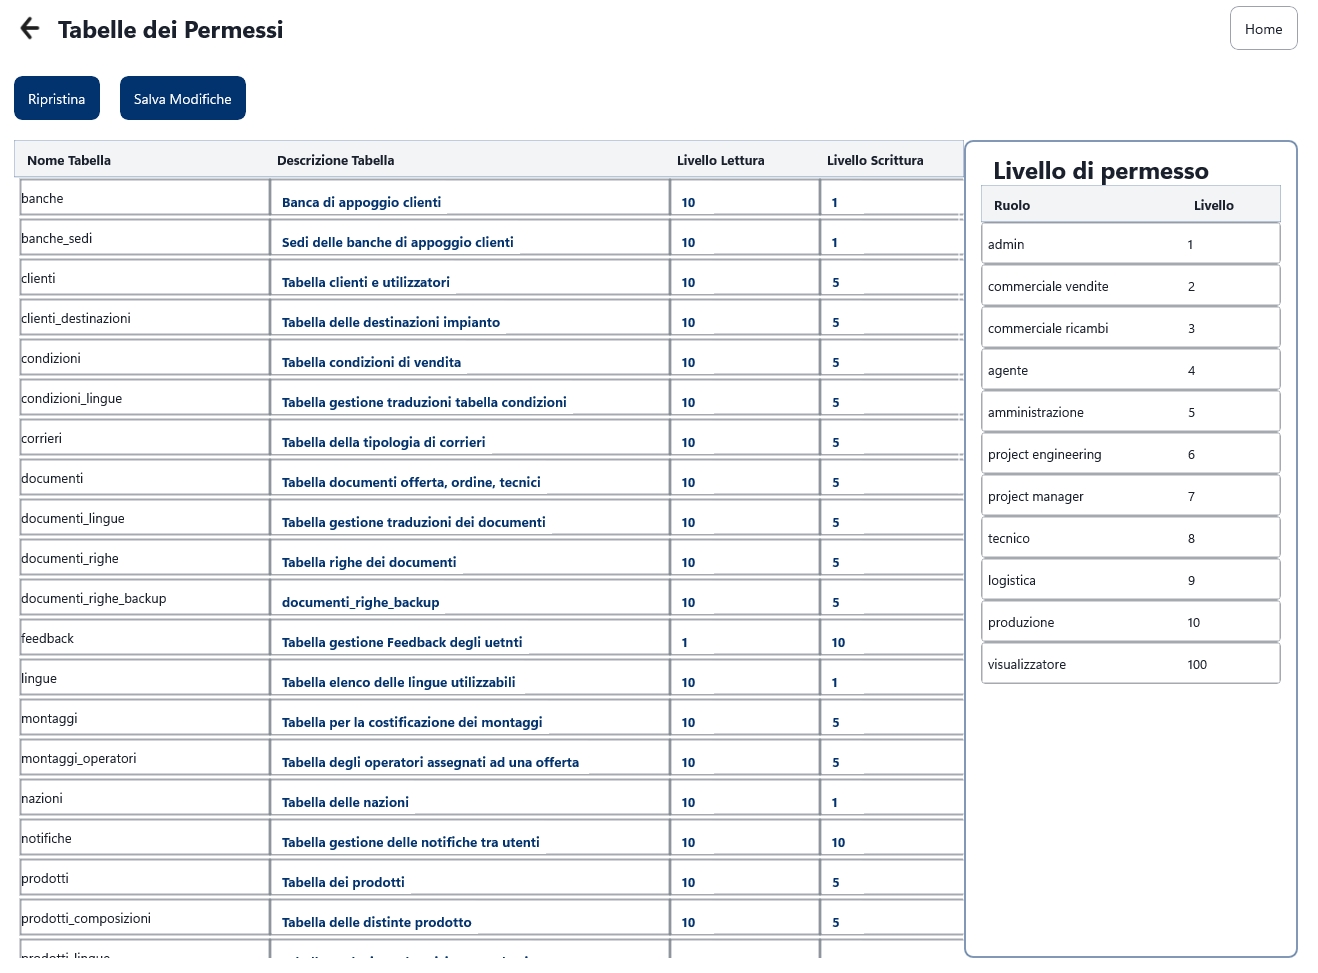
\includegraphics[width=0.8\linewidth]{figures/InterfacciaGestionePermessi.png}}
    \caption{Interfaccia di gestione dei permessi}\label{fig:GestionePermessi}
\end{figure}
In ottica offline, questa tabella permette di mappare, solo quello che l'utente
può modificare in locale, evitando di eseguire query su tabelle non permesse offline.

\subsection{Importazione dei dati e stored procedure}\label{section:importdata}
Come da analisi, è stato richiesto di prelevare e sincronizzare alcuni dati da altri database.
Prima della costruzione delle vere e proprie query di sincronizzazione, si sono
studiate le tabelle di provenienza per ricostruire un ambiente similare, facilitando la costruzione delle query.
In particolare, dal database Fusion, si è ricostruita la struttura di assegnazione dinamica delle proprietà ad un prodotto.
Tale struttura, ponendo la cardinalità N:M tra prodotti e proprietà con aggiunta del campo valore,
permette l'assegnazione e la creazione di nuove proprietà senza modificare la struttura del database.
Alla tabella ``Proprietà'' è associata la tabella ``Proprietà\_valori''
per la gestione dei valori standard della stessa.
Il diagramma \ac{ER} è mostrato in figura~\ref{fig:ERProdotti}.
Una volta ricostruite le strutture si sono create le seguenti stored procedure:
\begin{itemize}
    \item Da \ac{ERP} → importazione ed aggiornamento delle anagrafiche dei prodotti.
    \item Da \ac{ERP} → importazione ed aggiornamento delle anagrafiche dei listini.
    \item Da \ac{ERP} → importazione delle distinte dei prodotti.
    \item Da \ac{PLM} → importazione ed aggiornamento delle proprietà dei prodotti.
    \item Da \ac{PLM} → importazione dei valori standard associati alle proprietà dei prodotti.
\end{itemize}
Tutte le stored procedure hanno al loro interno dei controlli che permettono di
attuare le modifiche solo se presenti dei cambiamenti, evitando di sovraccaricare
il database con operazioni non necessarie.
Oltre a ciò saranno da prevedere altre stored procedure di importazione per la gestione di altri dati,
come ad esempio i clienti, tassi di cambio, ecc.
Una volta in produzione verranno schedulate giornalmente garantendo la sincronizzazione dei dati.
\subsection{Schema logico}
Lo schema logico risultante è visibile in figura~\ref{fig:SchemaLogico}.
\begin{figure}[H]
    \centering
    \fbox{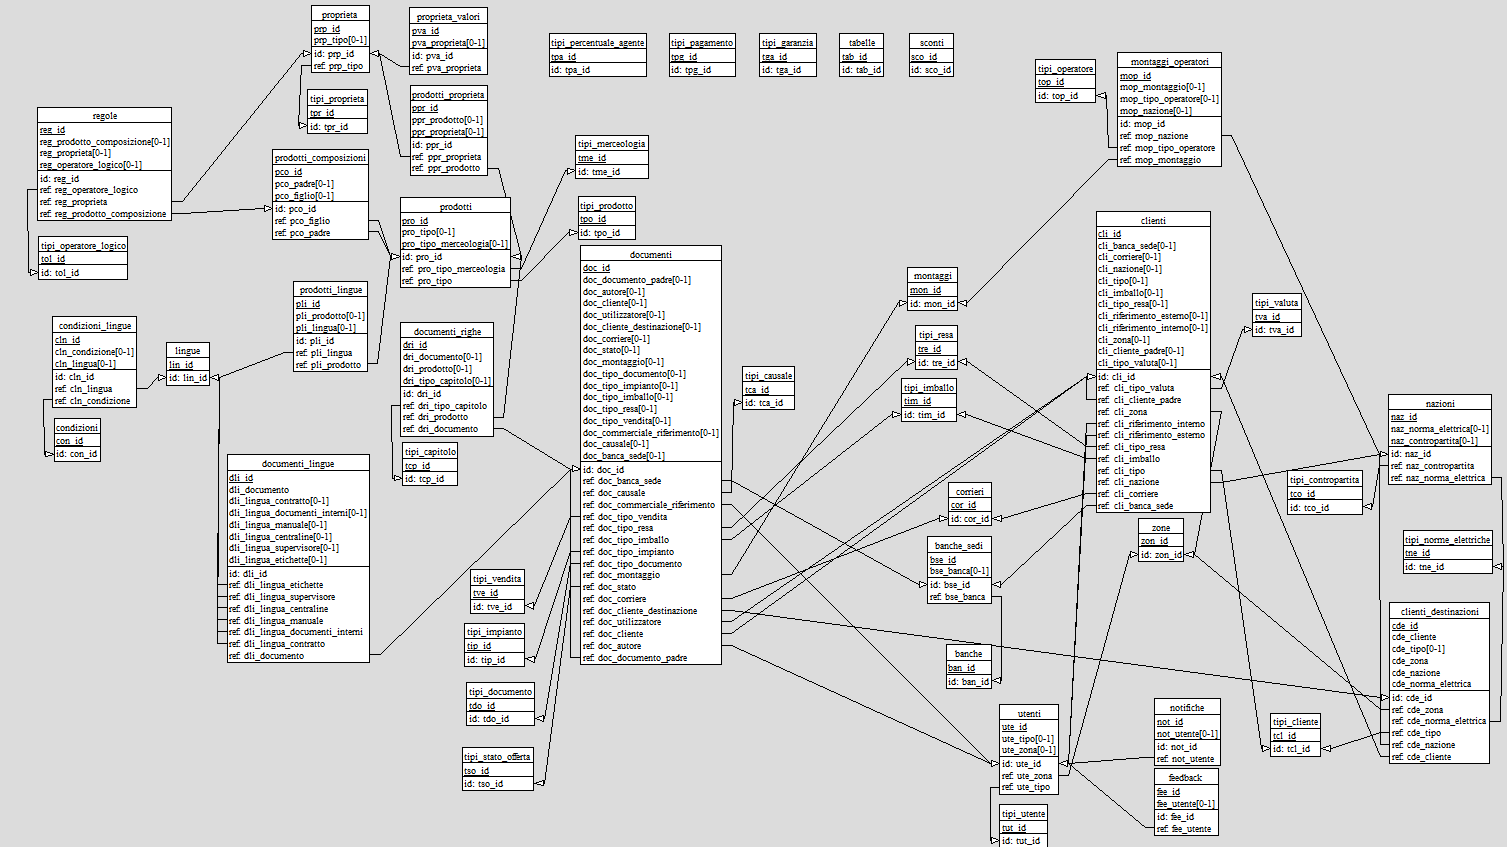
\includegraphics[width=1.3\linewidth, angle=90]{figures/Logical.png}}
    \caption{Schema logico del database}\label{fig:SchemaLogico}
\end{figure}

\chapter{Creazione del model}\label{chap:Model}
\section{Mapping delle classi}
Il model dell'applicativo è suddiviso in parte nel package
``DatabaseManagementPackage'' ed in parte, all'interno di quello principale.
Il package di interfaccia al database è stato realizzato mediante \ac{EF Core},
importando le tabelle del database sottoforma di classi entity.
Le classi entity sono una rapprosentazione delle tabelle del database, dove ogni classe rappresenta una tabella
ed ogni proprietà della classe rappresenta un campo della stessa.
Una volta generate le classi entity, si sono individuati gli oggetti fondamentali del dominio,
che sono stati mappati in classi \ac{DTO} mediante il package ``Mapster''.
I \ac{DTO} sono stati realizzati per essere utilizzati come oggetti neutri che non
esponessero direttamente le classi entity, e quindi il database, all'esterno del package.
Questi oggetti sono stati scelti in quanto rappresentano le entità principali del dominio,
come ad esempio ``Cliente'', ``Prodotto'' e ``Documento''.
Le classi \ac{DTO} sono state realizzate copiando la struttura delle entity di riferimento.
In corrispondenza dei campi legati ad altre tabelle mediante foreign key, sono stati adottati due approcci differenti.
Se il campo aveva un \ac{DTO} associato si richiamava quest'ultimo,
altrimenti sono stati mappati in oggetti \texttt{Dictionary<int,string>}, dove la chiave è l'\ac{ID} ed il valore è la descrizione.
Il mapping è bidirezionale per poter riconvertire, quando necessario, un \ac{DTO} in entity ed inserirlo nel database.
\section{Struttura del package}
Il package è stato strutturato in modo da separare gli ambienti di test da quelli di produzione.
All'esterno del package oltre alle classi \ac{DTO} e di Enumerazione relativi ad alcuni lookup, è
stata costituita una classe che raccoglie ed espone i repository.
La classe, denominata ``DatabaseManager'', si occupa di gestire le connessioni al database,
le transazioni e di esporre i vari repository.
Questa soluzione permette di avere un unico punto di accesso ai repository,
evitando di esporre le classi interne del package e facilitando la \ac{DI}.
La \ac{DI} è un design pattern che permette di iniettare le dipendenze necessarie ad una classe,
senza doverle istanziare all'interno della stessa.
Le classi iniettabili vengono registrate all'interno della classe che gestisce la \ac{DI}, talvolta come singleton,
in modo da avere un'unica istanza della classe per tutta la durata dell'applicativo.
Il singleton è un pattern creazionale che assicura l'esistenza di
una sola istanza di una determinata classe e mette a disposizione
un punto di accesso globale per utilizzarla.
Il ``DatabaseManager'', per garatire un solo accesso ai repository, è stato registrato come singleton.
Ad ogni repository è stata associata una classe di test, che ne verificasse in modo efficace i vari metodi.
La gestione dei dati dell'utente loggato è stata affidata ad una classe dedicata, anch'essa
registrata come singleton, che mantenesse le infomazioni della sessione dell'utente.
Tali informazioni includono, ad esempio l'\ac{ID} dell'utente, ll'anagrafica dello stesso, il ruolo per i permessi.
La classe in questione, unita alla tabella ``Tabelle'',
permette di intercettare la tipologia di richiesta, il livello dell'utente e
di conseguenza bloccare operazioni non permesse.
\subsection{Classi di test}
Le classi di test sono state pensate con l'obiettivo di funzionare anche in presenza di dati reali.
Per realizzare ciò si sono creati prima di ogni test dei savepoint del database,
che permettessero di tornare allo stato iniziale.
Successivamente, per ogni test, si sono creati i dati di test fittizi che potessero validare
le funzionalità del repository senza
il rischio di prelevare dati reali.
Questo approccio ha richiesto molto tempo per la ricostruzione dei test più complessi, ma
ha permesso di testare piccoli cambiamenti senza dover ripristinare il database.
A fronte del tempo impiegato prima si è utilizzata \ac{IA} generativa per creare le bozze dei test.
Tali bozze sono state successivamente modificate ed, in alcuni casi, riscritte completamente,
per adattarle al contesto reale.
Per realizzare ciò si è adottato un approccio articolato come segue:
\begin{enumerate}
  \item scrittura metodi del repository;
  \item generazione dei test sulla base dei metodi del repository;
  \item correzione dei test per renderli accurati e validi;
  \item correzione dei metodi del repository sulla base del risultato dei test.
\end{enumerate}
Questo approccio ha permesso di avere un ciclo di sviluppo più veloce,
riducendo il tempo di scrittura dei test.
\subsection{Repository}
I repository sono stati divisi in base alle entità principali del dominio,
come ad esempio i Prodotti, i Clienti ed i Documenti.
Oltre alle operazioni \ac{CRUD} principali è stato scelto, per quanto concerne le operazioni di ricerca,
di utilizzare dei metodi che permettessero di inserire molteplici criteri di ricerca.
All'interno sono poi stati utilizzati i \texttt{Queryable} per costruire la query in esame.
I \texttt{Queryable} permettono la costruzione pezzo per pezzo query complesse,
includendo solo i criteri necessari e riducendo la complessità delle stesse.
Con un unico metodo si possono  così costruire query complesse, evitando di scrivere molteplici
metodi per ogni combinazione di criteri.
Un esempio di query costruita con \texttt{Queryable} è riportata nel listato~\ref{lst:esempio-query-queryable}.
\lstinputlisting[
  language=CSharp,
  caption={Esempio di query Queryable},
  label={lst:esempio-query-queryable}
]{listings/Queryable.cs}
Tutti i metodi all'interno dei repository sono stati realizzati come asincroni,
per evitare di bloccare il thread principale dell'applicativo e, in particolare, l'interfaccia grafica.
\section{Gestione dei dati e delle transazioni}
Ogmi query al database è stata realizzata come transazione atomica,
in modo da evitare di lasciare dati parziali in caso di errori.
In questo modo ad ogni azione si apre e si chiude una transazione, eseguendo un commit automatico al termine della stessa.
I dati, prima dell'effettivo inserimento nel database,
vengono gestiti in memoria \ac{RAM} e solo al termine di tutte le operazioni, vengono salvati nel database.
Questo approccio permette di non impegnare il database con dati parziali,
e di conseguenza, di non dover gestire rollback in caso di errori.
Ad ogni metodo dei repository è stato aggiunto il parametro \texttt{CancellationToken}\cite{CancToken},
che permette di forzare l'interruzione dell'esecuzione di una query.
L'utilizzo del \texttt{CancellationToken} può essere osservato nella query di esempio~\ref{lst:esempio-query-linq},
dove viene passato come parametro al metodo \texttt{FirstOrDefaultAsync()}.
La scelta di utilizzare il \texttt{CancellationToken} è volta a permettere all'utente di interrompere
un'operazione in caso di necessità.
L'uso di questo parametro libera le risorse del database e lo rende disponibile per altre operazioni,
evitando di bloccare l'applicativo.
L'apertura di nuove interfacce richiede quasi sempre una interrogazione al database.
L'utilizzo del \texttt{CancellationToken} permette di cambiare
interfaccia bloccando l'operazione sulla precedente in favore della nuova.


\chapter{Creazione View}\label{chapter:View}
\section{Utilizzo di Figma per il disegno delle interfacce}
La prototipazione delle interfacce grafiche, è stata realizzata mediante l'utilizzo del software Figma\cite{Figma}.
Figma è una web application che permette di disegnare layout interattivi.
Un aspetto non secondario di Figma è la possibilità di esportare le interfacce sia in
formato vettoriale \ac{SVG} che con codice \ac{CSS}.
Questo aspetto, unito all'utilizzo dell'\ac{IA} generativa, ha permesso la conversione dei
codici \ac{CSS} e \ac{SVG} in codice
\csharp{} Markup, con un notevole risparmio di tempo.
Inizialmente si è deciso di prototipare solo le interfacce principali,
quali le schermate di login, ricerca e dettaglio di prodotti, clienti e preventivi.
Cercando di mantenere l'obiettivo progettuale orientato al cross-platform,
si è deciso di realizzare le schermate in modo da essere responsive,
e con un design mobile first. Si è quindi cercato di inserire tutti i comandi, escludendo
l'utilizzo della tastiera e del mouse, in quanto non sempre disponibili sui dispositivi mobili.
Sfruttando la compilazione condizionale, si è cercato di costruire dei layout specifici per alcuni dispositivi.
Alcuni filtri, sono ad esempio, collassati in un menù a tendina sui dispositivi mobili, mentre su desktop sono sempre visibili.
Nelle immagini che seguono si può osservare l'evoluzione dal prototipo in figura~\ref{fig:Prototipo Home Figma},
alla realizzazione finale delle interfacce grafiche in figura~\ref{fig:Interfaccia Desktop e Mobile}.
\begin{figure}[H]
    \centering
    \fbox{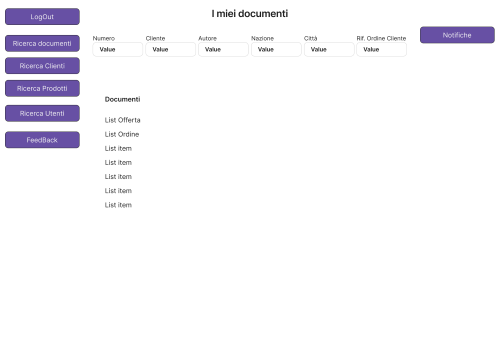
\includegraphics[width=0.9\linewidth]{figures/Figma.png}}
    \caption{Prototipo Home Figma}\label{fig:Prototipo Home Figma}
\end{figure}
\begin{figure}[H]
    \centering
    \fbox{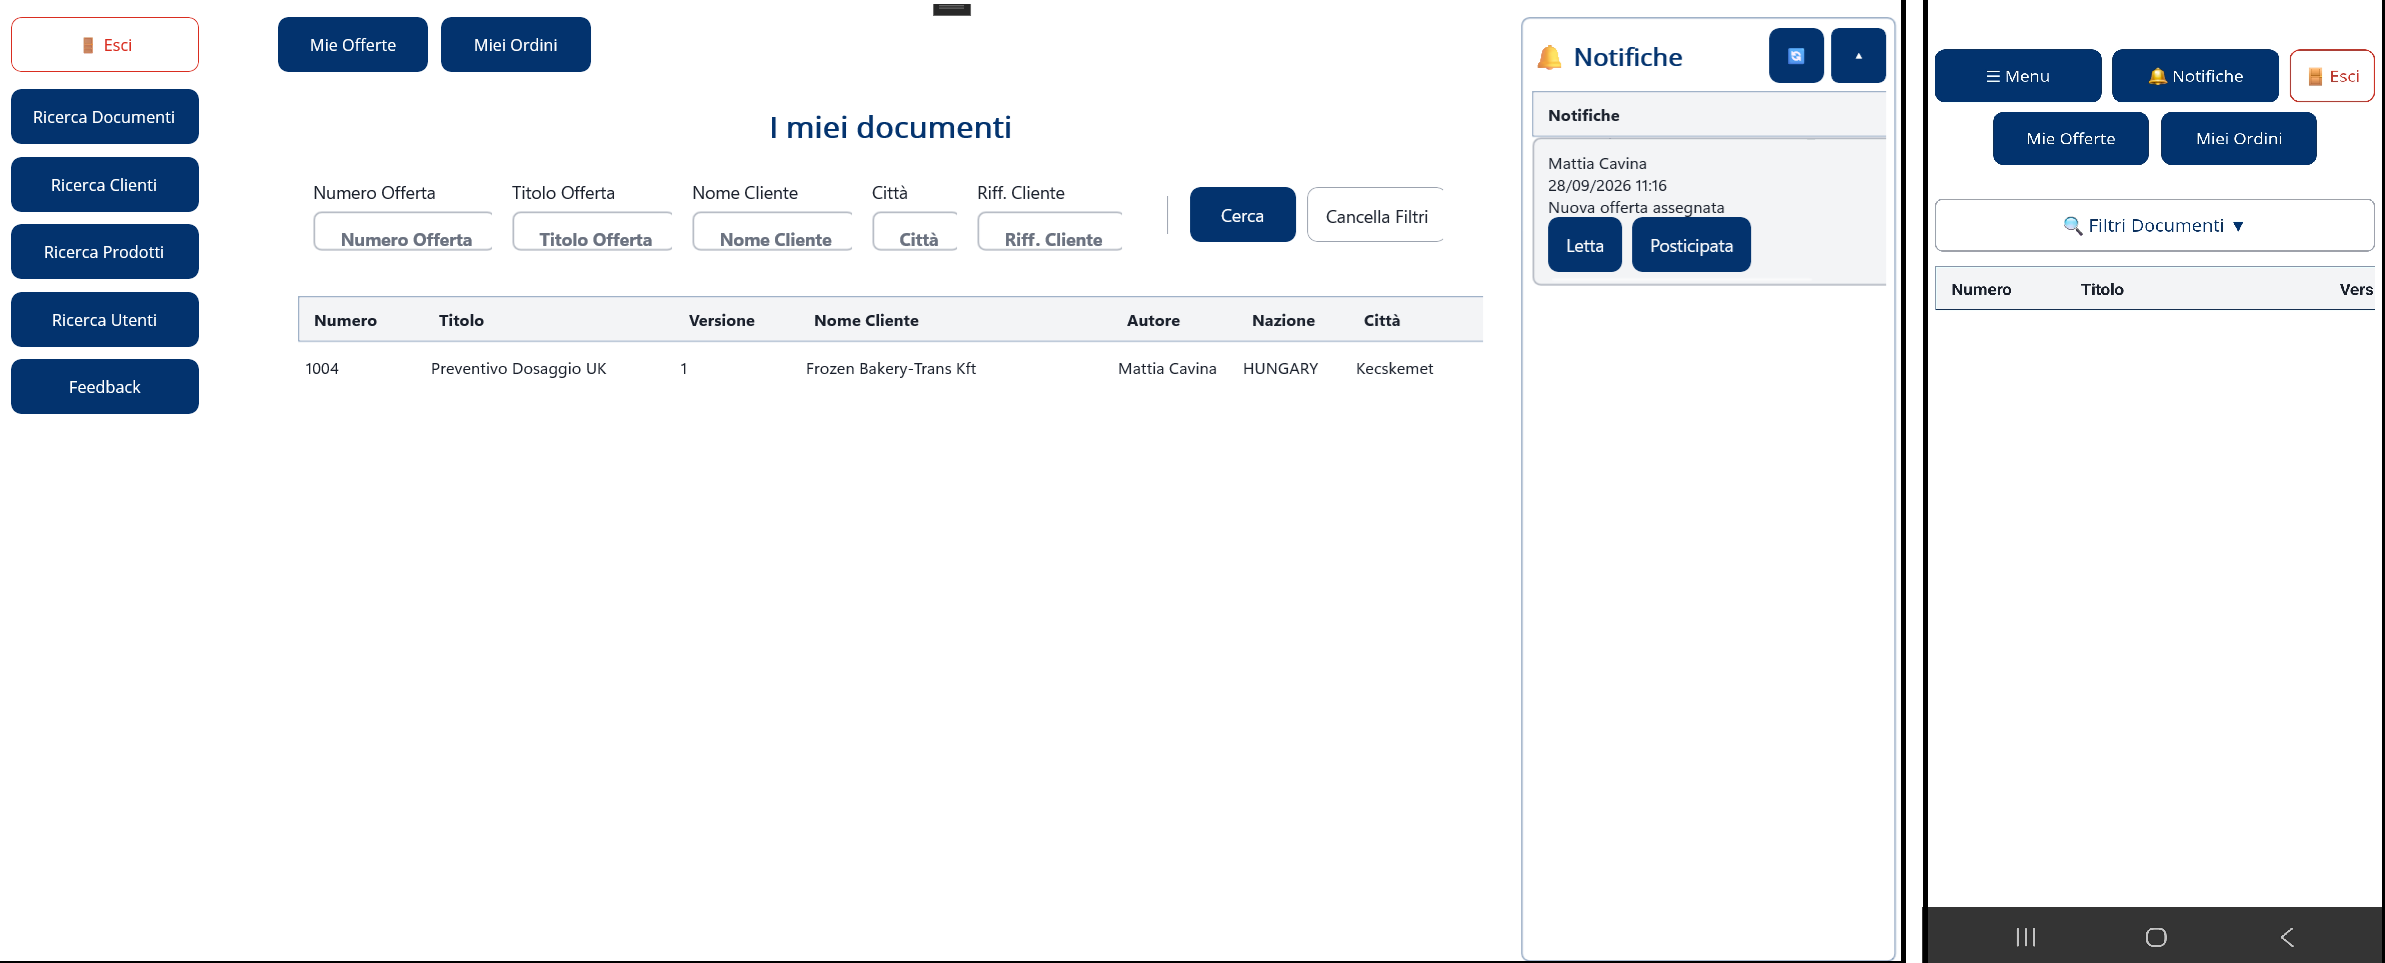
\includegraphics[width=0.9\linewidth]{figures/Realizzazione.png}}
    \caption{Interfaccia Desktop e Mobile}\label{fig:Interfaccia Desktop e Mobile}
\end{figure}
\section{Creazione delle Factory per le View}
A partire dalla versione prototipale, è stato stabilito fin dall'inizio di
raccogliere i componenti grafici in classi factory, che ne permettessero la creazione in modo centralizzato.
Il pattern Factory permette di astrarre la creazione delle view e di centralizzarne la logica di creazione.
Le factory principali realizzate sono le seguenti:
\begin{itemize}
    \item \textbf{Colori:} factory che espone i colori utilizzati nell'applicativo,
          permettendo di centralizzarne la gestione.
    \item \textbf{Componenti:} factory che espone i componenti grafici, come bottoni, etichette e caselle di testo.
    \item \textbf{Dimensioni:} factory che espone le dimensioni dei componenti grafici,
          come la loro larghezza e l'altezza tipica.
    \item \textbf{Popup di notifica:} factory che espone i metodi per la creazione di popup di notifica,
          come messaggi di errore o di conferma.
\end{itemize}
La centralizzazione ha permesso un ampio riutilizzo dei componenti,
oltre alla possibilità di ampliarne le funzionalità senza dover modificare dove già implementati.
Ciò è stato possibile gestendo un notevole numero di valori nullable,
che permettono di personalizzare i componenti in base alle esigenze.
\section{Scelta delle classi di ViewModel}
Interposti tra le view ed i repository, secondo il pattern \ac{MVVM} consigliato da \dotnet,
si sono creati i ViewModel.
Queste classi hanno il compito di prelevare i dati dai repository ed esporli alle view, tramite proprietà osservabili.
Le proprietà osservabili permettono di aggiornare automaticamente le view al variare dei propri dati.
All'interno dei ViewModel, infatti, sono racchiuse proprietà e liste osservabili dedicate al compito prima descritto.
I ViewModel non sono stati creati in rapporto uno ad uno con le view,
ma piuttosto seguendo criteri basati sulla loro funzionalità e sull'elemento del dominio da gestire.
Ad esempio, nella gestione dei prodotti sono stati creati due
ViewModel, uno per la gestione semplice dei prodotti ed uno delle relative distinte.
Le view create che utilizzano tali ViewModel sono molte di più.
Questo approccio, unito all'estendibilità delle classi, ha permesso di avere un numero limitato
di ViewModel in rapporte alle view.
Nel processo di rifattorizzazione si è notata la presenza di elementi comuni nei ViewModel.
Un esempio di elementi comuni è la gestione delle liste dedicate ai dropdown, dei filtri e dei messaggi di notifica.
Si è quindi creato un ViewModel base, che racchiudesse i metodi e le proprietà comuni a tutti i ViewModel.
Questi ultimi, a loro volta, estendono il ViewModel base e aggiungono le specificità necessarie.
In alcuni casi si è effettuato un override dei metodi base, gestendo comportamenti particolari.
Un esempio di override è la gestione della selezione da dropdown.
ViewModel differenti che richiamano una stessa lista per un dropdown richiedono che il risultato
della selezione finisca in differenti oggetti.
Nella pratica, ad esempio, il menù di selezione degli utenti può fungere
da selezione di un autore per un documento o di un destinatario per una notifica.

\chapter{Modulo di configurazione prodotto}\label{chapter:Configurazione}
\section{Scopo del modulo}
L'introduzione della configurazione di prodotto all'interno del sistema,
ha come scopo quello di unire il processo di vendita con quello di produzione.
Come anticipato nell'introduzione~\ref{chapter:introduction}, l'azienda adotta un modello di business
di tipo \ac{ETO}. Tale modello prevede la realizzazione di prodotti su misura per il cliente, ma
utilizzando componenti standardizzati.
Quest'ultimi hanno un codice, delle giacenze a magazzino ed un prezzo
di listino per la vendita o l'acquisto.
L'utilizzo dei componenti consente di individuare e catalogare
le possibili varianti di prodotto. Attraverso le configurazioni è possibile,
suggerire una pianificazione di produzione.
Le tipologie di macchine prodotte dall'azienda sono numerose e per ciascuna di esse, esistono molteplici varianti.
Non si può quindi pensare di gestire le configurazioni in maniera statica, ma è necessario
predisporre un sistema dinamico.
È stato necessario progettare una struttura del database agile,
che consentisse al lato utente di operare in maniera dinamica.
È stato progettato un algoritmo che desse all'ammministratore la possibilità di creare regole e combinarle agilmente.
Lo stesso algoritmo, in fase di configurazione, consente all'utente di comporre il prodotto
filtrando le regole prima definite.
Allo scopo di guidare l'operatore nella scelta del prodotto da configurare,
è stato predisposto un sistema di alberi decisionali, che consente di scendere da concetti generali fino al modello specifico.
Prima di procedere con l'esposizione dettagliata del modulo, è necessario introdurre il concetto di Macrogruppo.
Esso è un contenitore logico di tutti i possibili componenti potenzialmente impiegabili nella configurazione.
A ciascuno di essi sono associate una o più regole che ne determinano l'effettiva disponibilità.
All'interno sono presenti anche elementi di tipologia ``listino''.
Questi componenti concorrono a definire il prezzo del prodotto.
L'algoritmo implementato si suddivide in quattro fasi principali:
\begin{itemize}
    \item Fase di scelta del modello: mediante alberi decisionali
          l'utente discende da concetti generali, come lo scopo del componente (es: ``stoccaggio prodotti''),
          fino alla tipologia di prodotto (es: ``silo in acciaio''), per giungere al modello specifico
          da configurare (es: ``forma quadrata'').
    \item Fase di configurazione: vengono proposte all'utente opzioni di scelta
          sotto forma di menù a tendina o campi a testo libero.
          Ogni selezione corrisponde ad una specifica proprietà utilizzata nelle regole del prodotto.
          Il menù viene generato dinamicamente filtrando le proprietà associate alle regole
          in base al Macrogruppo selezionato.
          Ogni menù a sua volta, propone all'utente soltanto i valori delle proprietà
          effettivamente utilizzati nella configurazione del prodotto, evitando di mostrare opzioni non pertinenti.
          Questa tecnica consente di guidare l'utente con un esiguo numero di scelte,
          evitando di esporlo ad un numero eccessivo di opzioni non necessarie.
    \item Fase di scelta dei componenti: una volta compilate le scelte precedenti,
          i componenti del Macrogruppo vengono filtrati in base alle regole associate a ciascuno di essi.
          In questo modo vengono proposti all'utente soltanto i componenti conformi alle regole,
          quindi effettivamente disponibili per la configurazione. Tali componenti possono essere
          ulteriormente esclusi manualmente dall'operatore.
    \item Fase di generazione del codice: rappresenta il passaggio più critico
          dell'algoritmo. In base ai componenti selezionati, si aprono due scenari possibili:
          \begin{itemize}
              \item Configurazione esistente: si verifica nel database se è presente
                    una configurazione di quel prodotto con le medesime caratteristiche.
                    In caso positivo, si propone all'utente di riutilizzarla.
              \item Configurazione inesistente: in caso negativo, viene generato
                    un nuovo codice identificativo di configurazione per il prodotto,
                    che viene contestualmente salvato a database.
                    Ad esso vengono associati tutti i prodotti prima filtrati.
          \end{itemize}
\end{itemize}
L'algoritmo descritto è visibile in figura~\ref{fig:Algoritmo configuratore}.
\begin{figure}[H]
      \centering
      \fbox{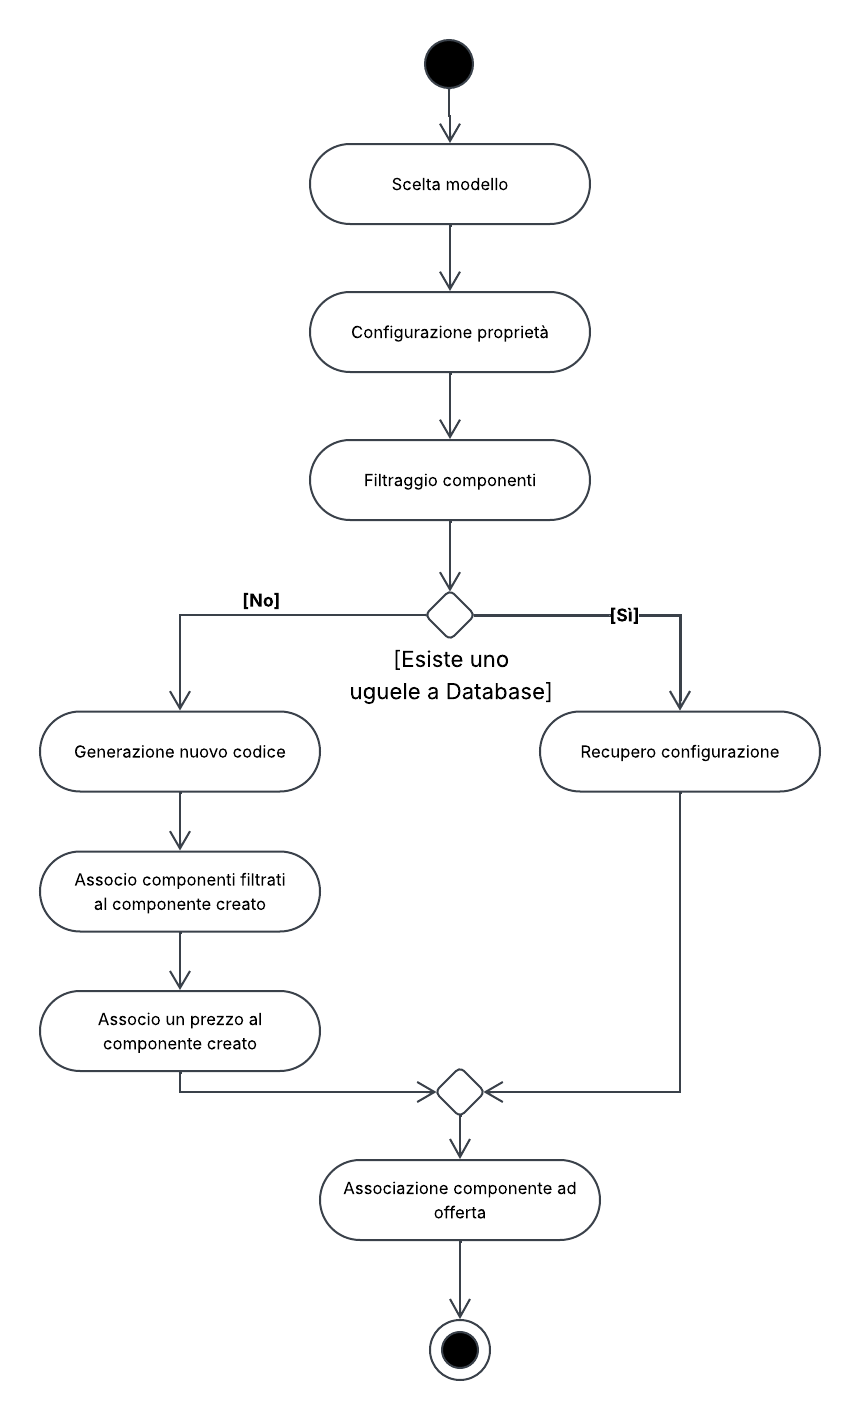
\includegraphics[width=0.5\linewidth]{figures/AlgoritmoConfiguratore.png}}
      \caption{Algoritmo di configurazione}\label{fig:Algoritmo configuratore}
\end{figure}

\subsection{Scelta del Macrogruppo da configurare}
La realizzazione dell'albero di scelta è stata condotta sfruttando
le tabelle già presenti nel database, in particolare le tabelle ``prodotto'', ``prodotti\_composizioni''
e la tabella di lookup ``tipi\_prodotto''.
Sono state introdotte quattro nuove tipologie di prodotto:
\begin{itemize}
    \item \textbf{Iniziale:} rappresenta il concetto generale del prodotto e costituisce il punto di partenza
          per l'algoritmo di configurazione, guidando l'utente verso la selezione del modello.
    \item \textbf{Mappa:} rappresenta un livello intermedio dell'albero. Questi prodotti, sono inseriti
          all'interno delle distinte base dei prodotti di tipo iniziale. Essi possono contenere a loro volta
          altri nodi di tipo mappa o Macrogruppo, consentendo la discesa gerarchica.
    \item \textbf{Macrogruppo:} rappresenta il contenitore logico dei componenti del modello da configurare.
          Ad ogni prodotto del Macrogruppo sono associate regole che ne determinano l'effettiva disponibilità.
          Questi elementi sono inseriti nelle distinte base dei prodotti di tipo mappa.
    \item \textbf{Listino:} rappresenta un elemento di prezzo minimo, che non concorre alla composizione fisica del prodotto.
          Anch'esso è soggetto alle regole del Macrogruppo e viene attivato in base alle scelte dell'utente.
\end{itemize}
Questa struttura assicura un'elevata scalabilità, poiché consente di censire nuovi prodotti
senza dover intervenire sul codice dell'algoritmo o sulla struttura del database.
L'albero in oggetto è illustrato in figura~\ref{fig:Albero di scelta prodotto}.
\begin{figure}[H]
    \centering
    \fbox{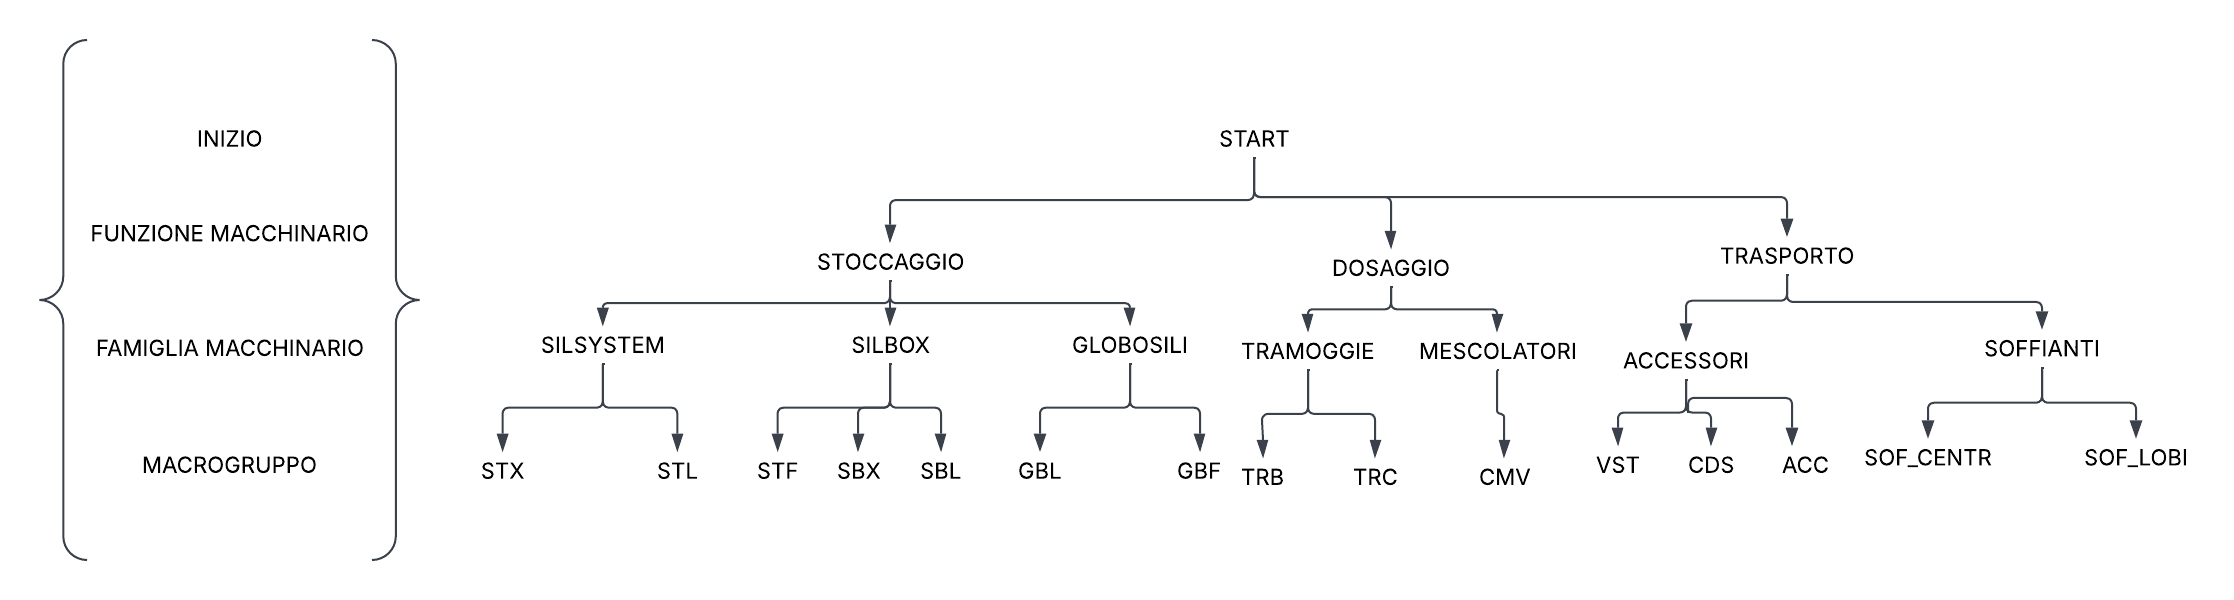
\includegraphics[width=1\linewidth]{figures/AlberoScelte.png}}
    \caption{Albero di scelta prodotto}\label{fig:Albero di scelta prodotto}
\end{figure}

\subsection{Implementazione delle regole}
I Macrogruppi contengono tutti i componenti potenzialmente impiegabili nella configurazione.
Ad ogni componente sono associate n regole che, se soddisfatte, ne determinano l'inclusione.
A ciascuna regola corrisponde una proprietà di riferimento, un operatore logico e un valore atteso.
Un esempio di regola è il seguente: ``Se la proprietà \textit{Altezza} è maggiore di 1000, allora il componente \textit{Pannello di rinforzo} è disponibile''.
Un secondo esempio riguarda una specifica normativa elettrica che impone particolari certificazioni in determinati paesi.
I due motori in questione potrebbero avere rispettivamente le seguenti regole:
\begin{itemize}
    \item MOT1-MERCATO-AMERICANO: ``Se la proprietà \textit{Normativa Elettrica} è uguale a \textit{UL-CSA},
          allora il motore è disponibile''.
    \item MOT2-MERCATO-EUROPEO: ``Se la proprietà \textit{Normativa Elettrica} è uguale a \textit{ATEX},
          allora il motore è disponibile''.
\end{itemize}
Si nota come le due opzioni, in base al valore assegnato alla proprietà, risultino mutuamente esclusive.

Le proprietà possono essere definite dall'utente configuratore; contestualmente, è possibile preimpostare
dei valori standard che vengono proposti all'utente durante la creazione della regola.
Gli operatori possono essere di confronto (ad esempio ``uguale a'', ``maggiore di'', ``minore di'')
o di corrispondenza (come l'operatore \texttt{LIKE}).
Nel caso dell'operatore di uguaglianza viene mostrato un menù a tendina popolabile con solo i valori standard.
Gli altri operatori, a differenza del precedente, consentono l'inserimento di un valore libero
o la selezione da una lista di valori ammessi.

\subsection{Generazione dell'interfaccia utente}
L'interfaccia con i parametri di configurazione, viene generata filtrando dinamicamente
tutte le proprietà di riferimento delle regole associate al Macrogruppo selezionato.
Viene eseguita una clausola di \textit{JOIN} tra componenti, regole e proprietà, isolando poi queste ultime
tramite l'operatore \textit{DISTINCT}, in modo da ottenere un insieme di proprietà univoche.
Questa query consente di ricavare le proprietà necessarie a runtime, senza vincolare il sistema
ad una conoscenza a priori delle regole che governano il prodotto.
I valori proponibili per ciascuna proprietà, sono ricavati solo tra quelli
effettivamente utilizzati nelle regole del Macrogruppo,
evitando di mostrare opzioni non pertinenti.

\subsection{Struttura del database}
L'architettura lato database, è stata realizzata introducendo due nuove tabelle:
la tabella ``Regole'' e la tabella di lookup ``Tipi\_operatori\_logici''.
La prima associa ad una riga del componente una proprietà, un operatore logico ed un valore atteso.
La seconda contiene l'elenco degli operatori logici ammessi.
La modellazione dinamica del database adottata, fin dalle prime fasi, ha consentito un'integrazione agevole.
In figura~\ref{fig:ER configuratore} è riportato lo schema \ac{ER} del modulo di configurazione.
\begin{figure}[H]
    \centering
    \fbox{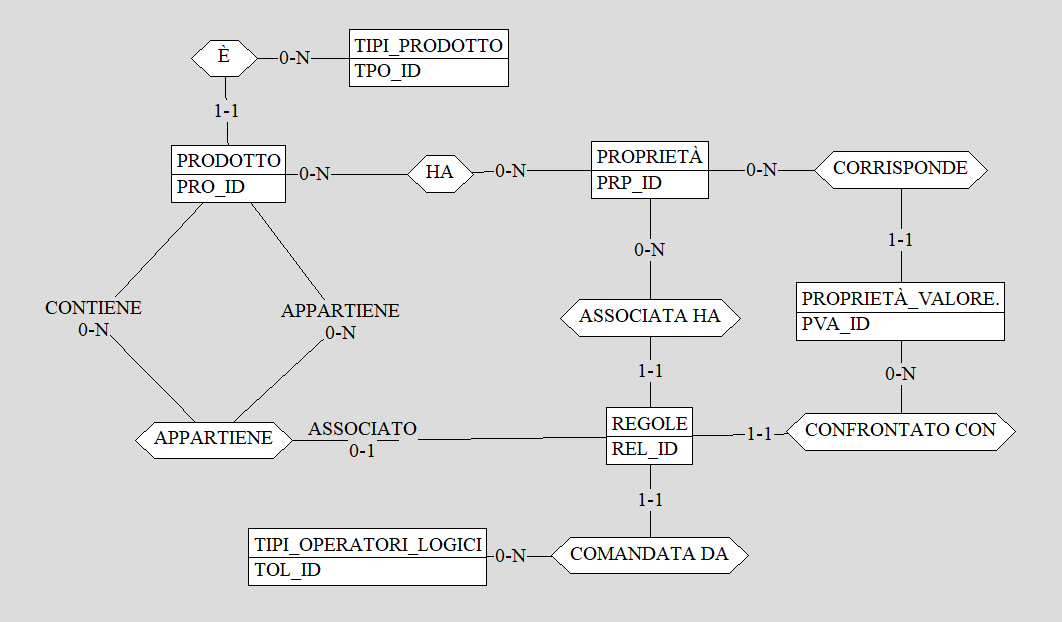
\includegraphics[width=0.9\linewidth]{figures/ER_Configuratore.png}}
    \caption{Modello ER del configuratore}\label{fig:ER configuratore}
\end{figure}

\subsection{Gestione del listino della configurazione}
Determinare il prezzo di una configurazione dinamica è un'operazione complessa,
poiché l'importo finale può dipendere sia dal prezzo dei singoli componenti scelti,
sia da soglie minime di listino.
Il problema è stato risolto introducendo un nuovo tipo di elemento di tipologia \textit{listino},
che contiene il prezzo minimo garantito per la configurazione.
Ciascun elemento di tipo listino è soggetto alle medesime regole degli altri componenti
e viene quindi attivato in base alle scelte dell'utente.
Questo approccio, consente di verificare se la somma dei prezzi dei singoli componenti scelti risulti inferiore
al prezzo minimo di listino, applicando in tal caso la soglia minima garantita.
I record di tipo listino restano invisibili all'utente finale, poiché non concorrono alla composizione fisica del prodotto.
Il flusso di assegnazione dei prezzi è illustrato in figura~\ref{fig:configuratore-listino}.
\begin{figure}[H]
    \centering
    \fbox{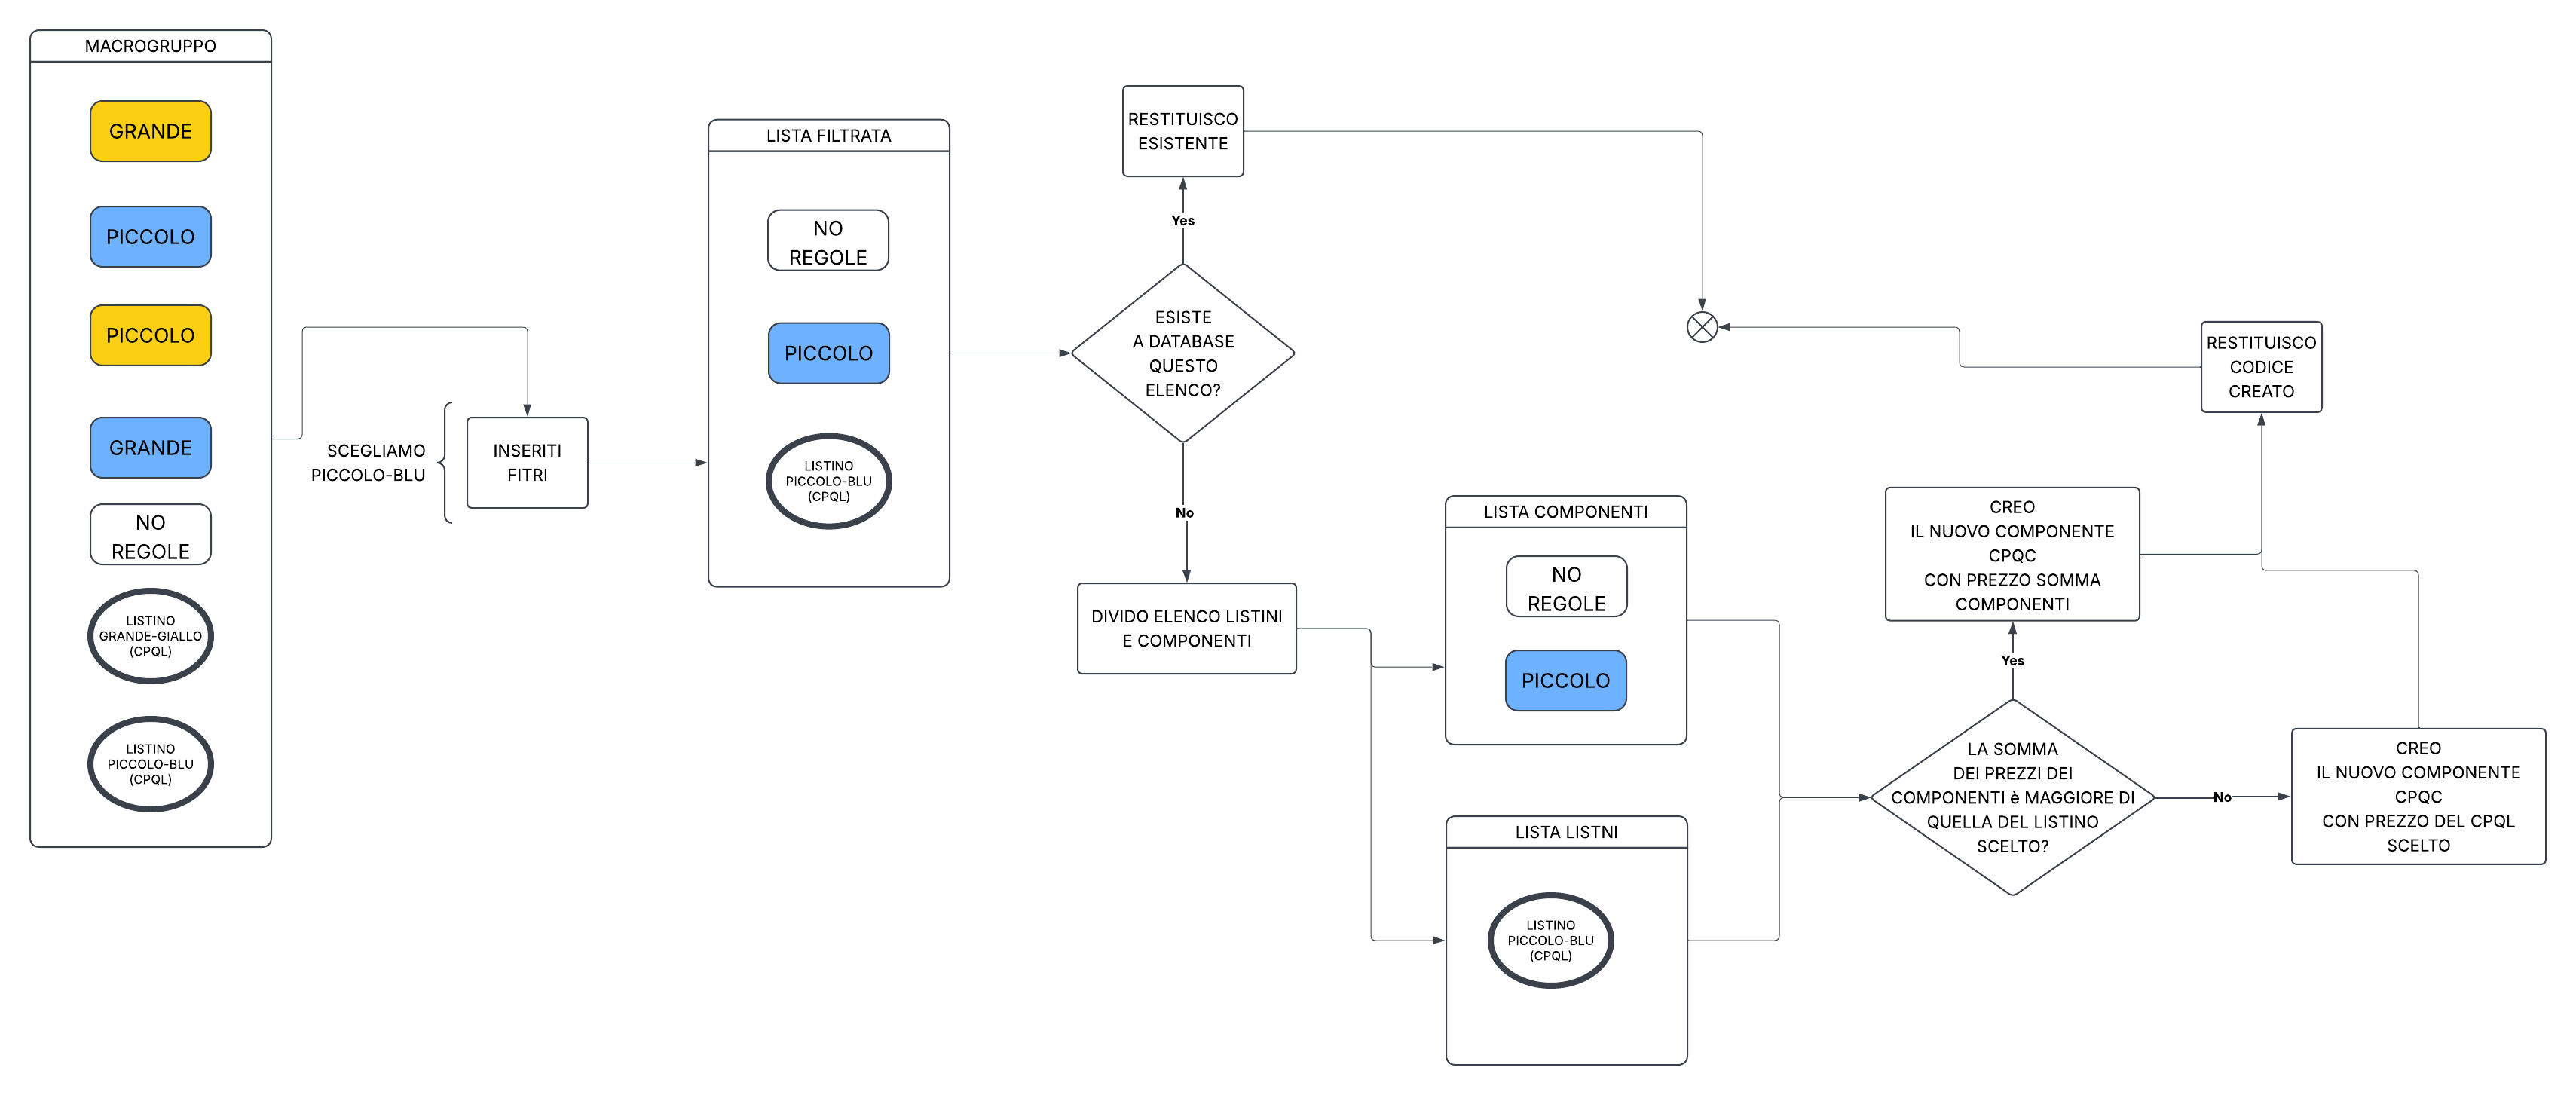
\includegraphics[angle=90, width=0.55\linewidth]{figures/Flowcharts.png}}
    \caption{Flusso di configurazione listino}\label{fig:configuratore-listino}
\end{figure}
Nello schema si può notare come, a partire da una situazione iniziale, dove sono presenti tutte le tipologie di componenti,
l'algoritmo filtri i componenti raccogliendo sia i componenti disponibili che le soglie minime di listino.
In base al risultato ottenuto, viene calcolato il prezzo finale della configurazione scegliendo il
maggior valore tra la somma dei prezzi dei componenti e la soglia minima di listino.

\section{Interfaccia grafica lato utente ed amministratore}
Le interfacce utente ed amministrativa presentano logiche profondamente differenti.
Al fine di garantire all'utente un'esperienza lineare e guidata,
la complessità della gestione è stata interamente demandata all'ambiente di amministrazione.

\subsection{Lato utente}
Il flusso di configurazione lato utente è stato progettato a valle di una sessione di focus group,
mirata ad individuare il percorso operativo più intuitivo.
Si è optato per abilitare la scelta sequenzialmente successiva, dell'abero di discesa,
solo dopo la conferma del passaggio precedente.
In questo modo si procede dalla comprensione del problema (lo scopo d'uso) fino alla definizione del modello specifico.
In figura~\ref{fig:Configurazione lato utente} è illustrata l'interfaccia presentata all'utente durante la selezione.
\begin{figure}[H]
    \centering
    \fbox{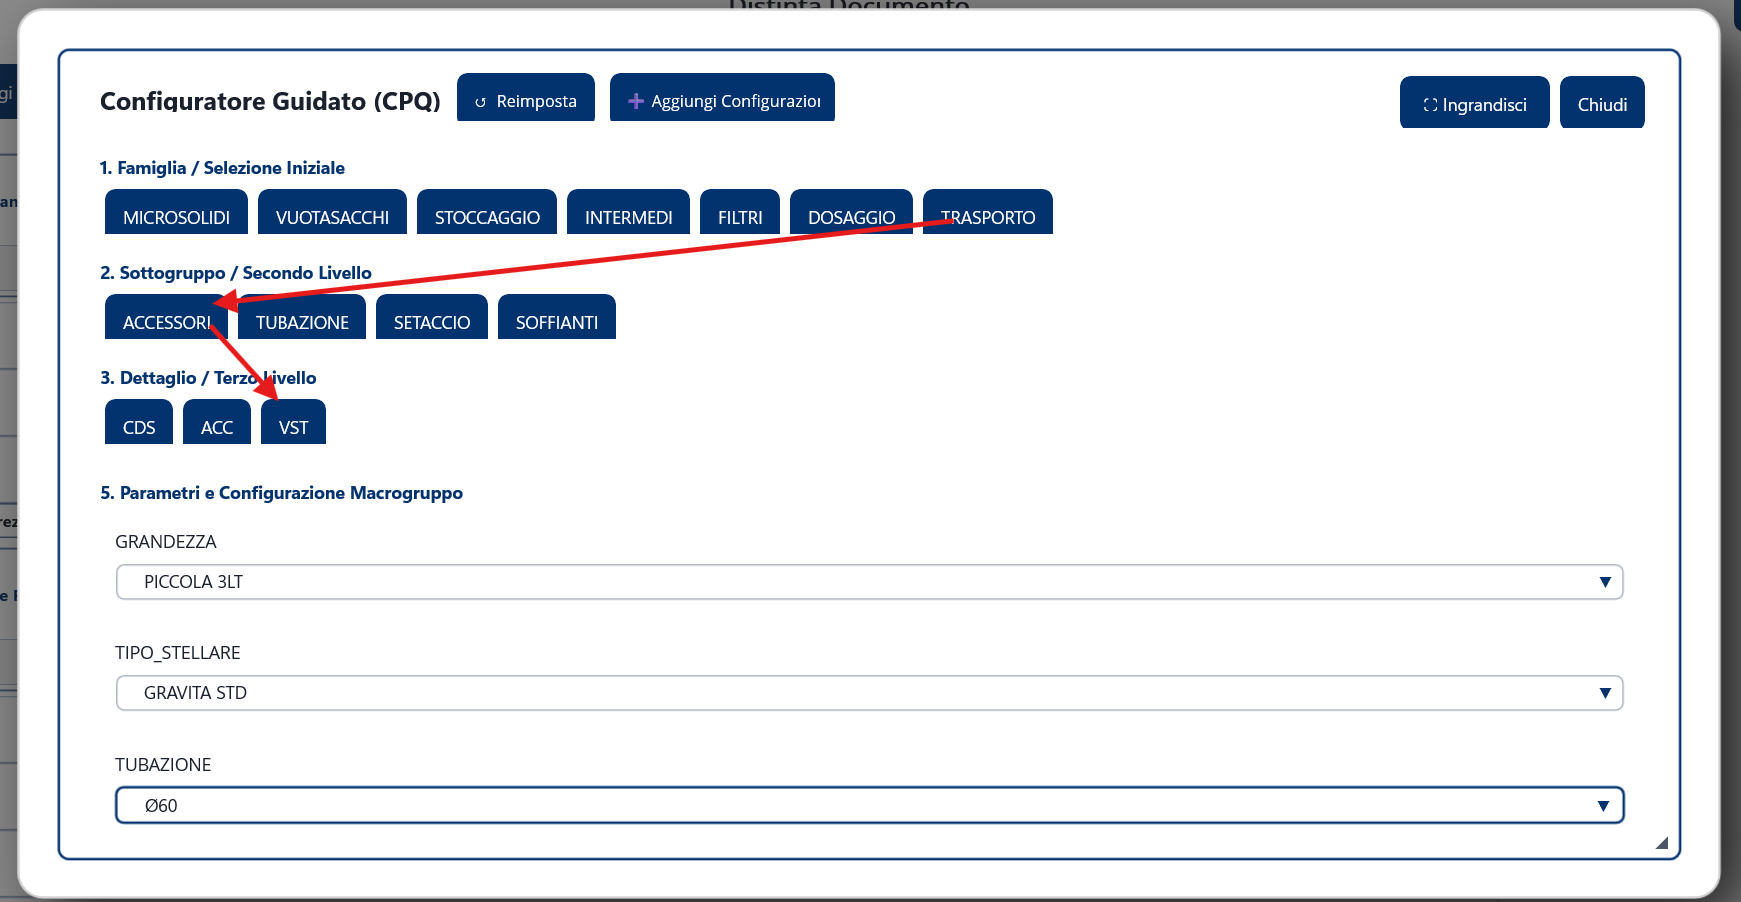
\includegraphics[width=0.9\linewidth]{figures/ConfigurazioneLatoUtente.png}}
    \caption{Configurazione lato utente}\label{fig:Configurazione lato utente}
\end{figure}
Il risultato al termine della procedura è visibile in figura~\ref{fig:Risultato configurazione lato utente}.
\begin{figure}[H]
    \centering
    \fbox{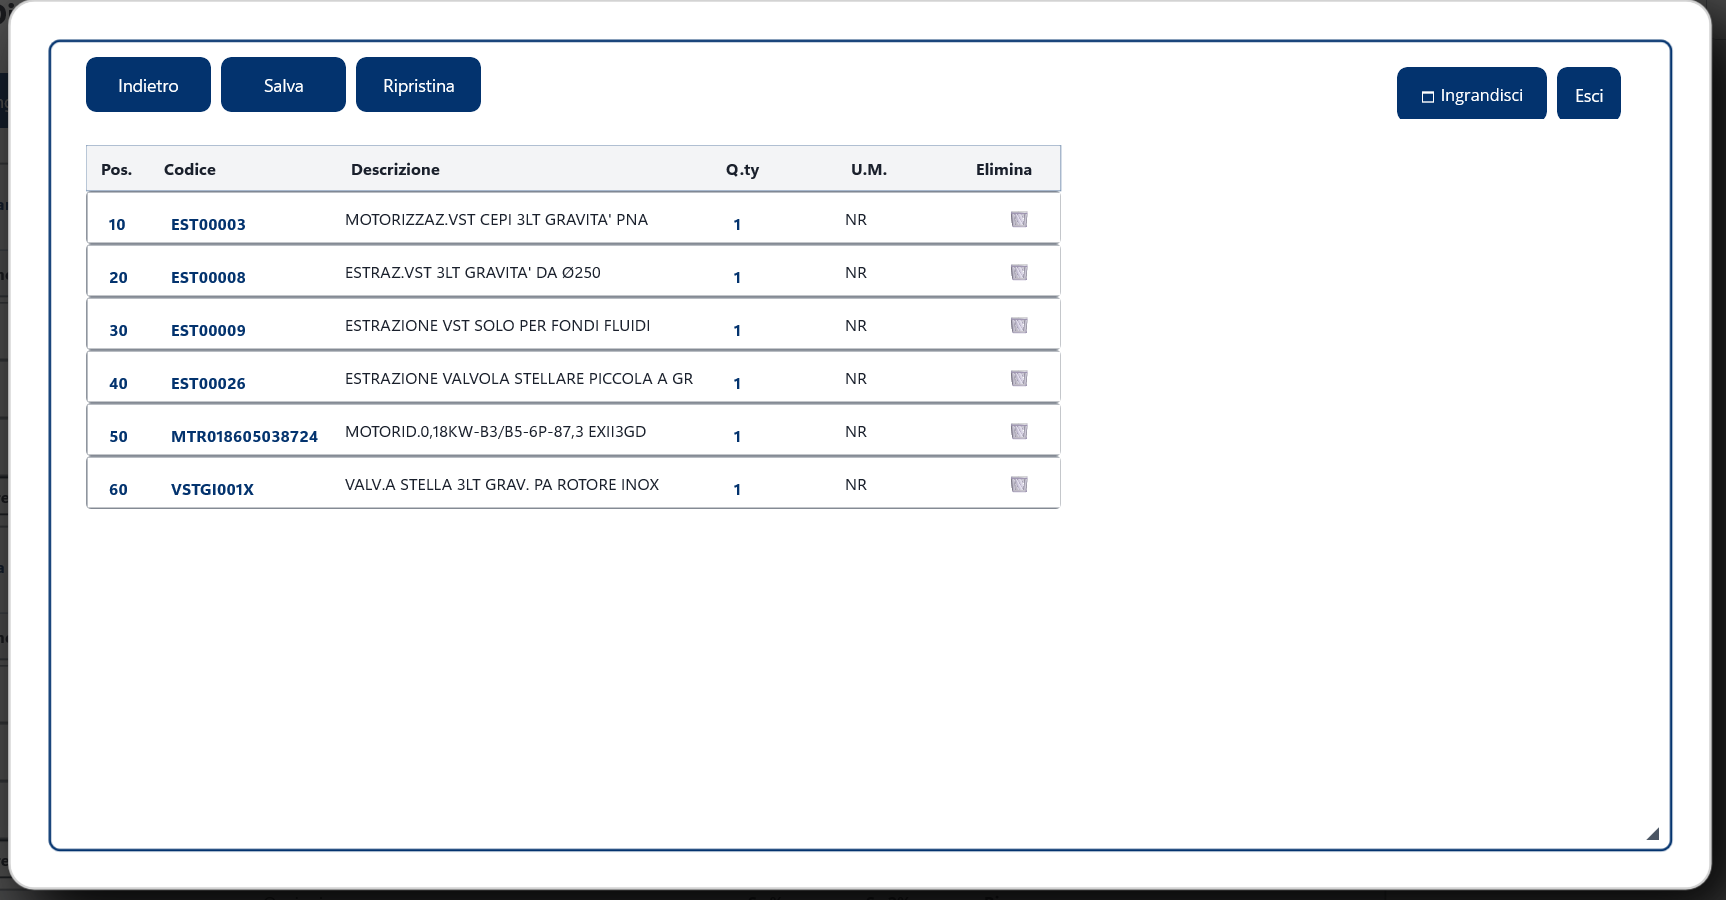
\includegraphics[width=0.9\linewidth]{figures/RisultatoConfigurazione.png}}
    \caption{Risultato configurazione lato utente}\label{fig:Risultato configurazione lato utente}
\end{figure}
Al termine, il codice prodotto generato (o recuperato dallo storico a database) viene inserito
tra le righe dell'offerta commerciale.

\subsection{Lato amministratore}
La definizione delle configurazioni avviene attraverso la composizione dei Macrogruppi.
Una volta associati i componenti al Macrogruppo, a ciascuno di essi possono essere applicate una o più regole.
L'assegnazione prevede la selezione della proprietà, dell'operatore logico e del valore
richiesto per abilitare il componente.
In figura~\ref{fig:Aggiunta regole lato amministratore} è riportata la schermata di gestione
delle regole per singolo componente:
\begin{itemize}
    \item sul lato destro sono presenti le proprietà già impiegate nella configurazione
          di almeno un altro componente del Macrogruppo.
          Tali proprietà possono essere utilizzate per generare una regola.
          Se necessario utilizare una proprietà non presente nell'elenco, è possibile crearne una nuova.
    \item sul lato sinistro sono presenti le regole associate al componente.
\end{itemize}
\begin{figure}[H]
    \centering
    \fbox{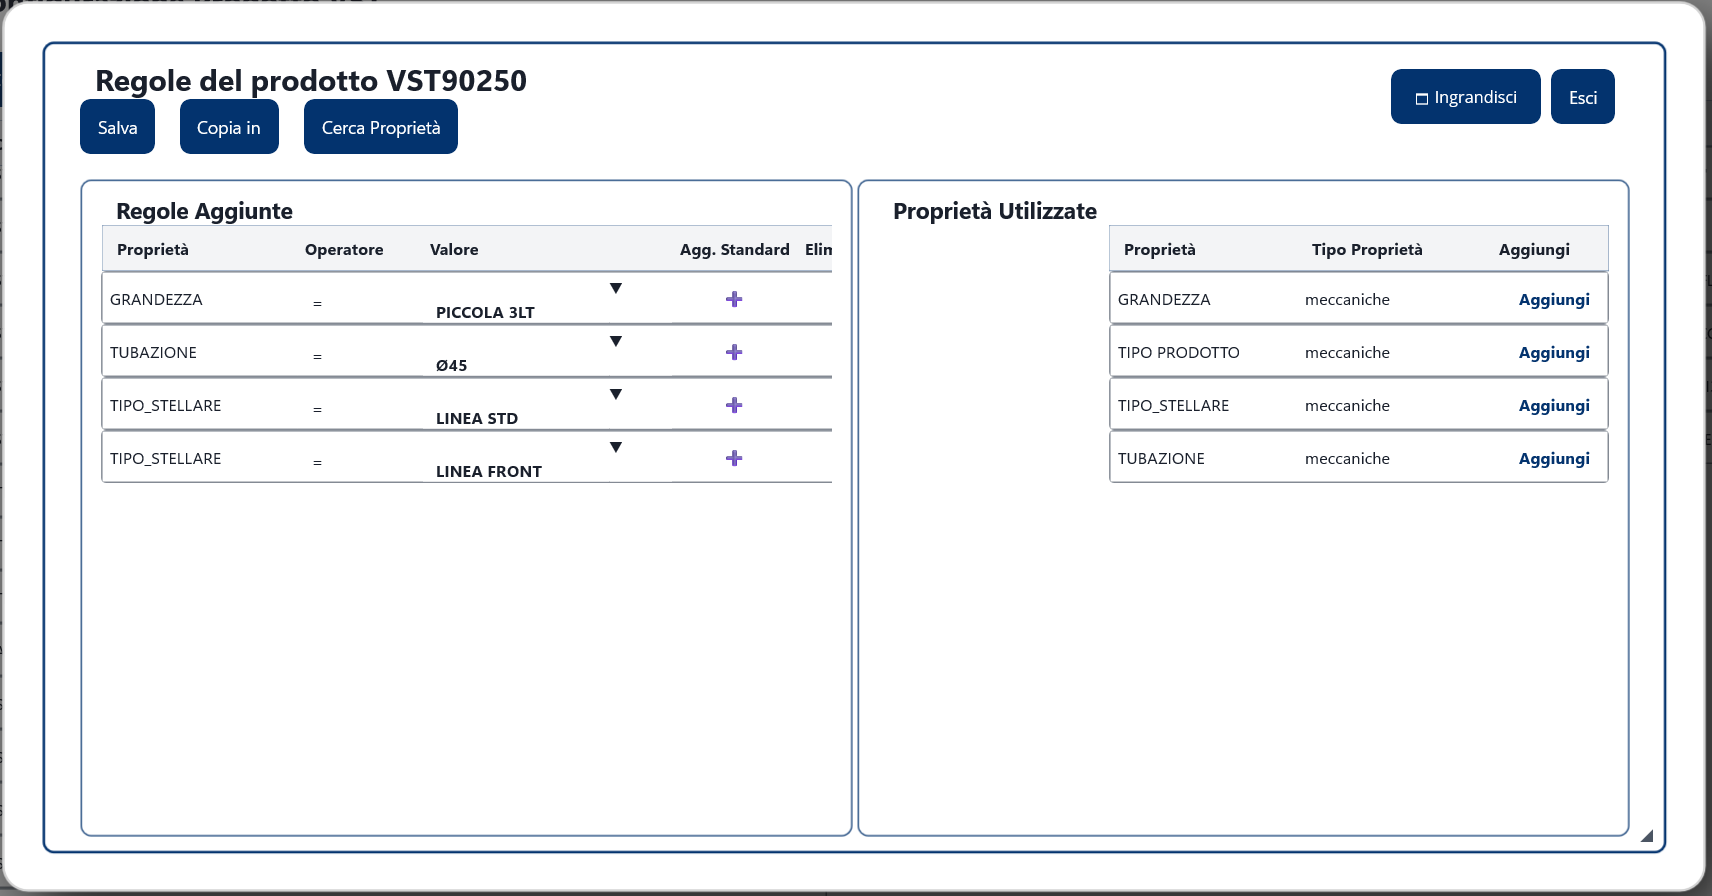
\includegraphics[width=0.9\linewidth]{figures/AggiuntaRegole.png}}
    \caption{Aggiunta regole lato amministratore}\label{fig:Aggiunta regole lato amministratore}
\end{figure}
Durante il focus group con gli utenti amministratori, è emersa l'esigenza
di validare preventivamente le regole. È stata pertanto implementata un'interfaccia dedicata al collaudo
della configurazione, illustrata in figura~\ref{fig:Test regole lato amministratore}.
\begin{figure}[H]
    \centering
    \fbox{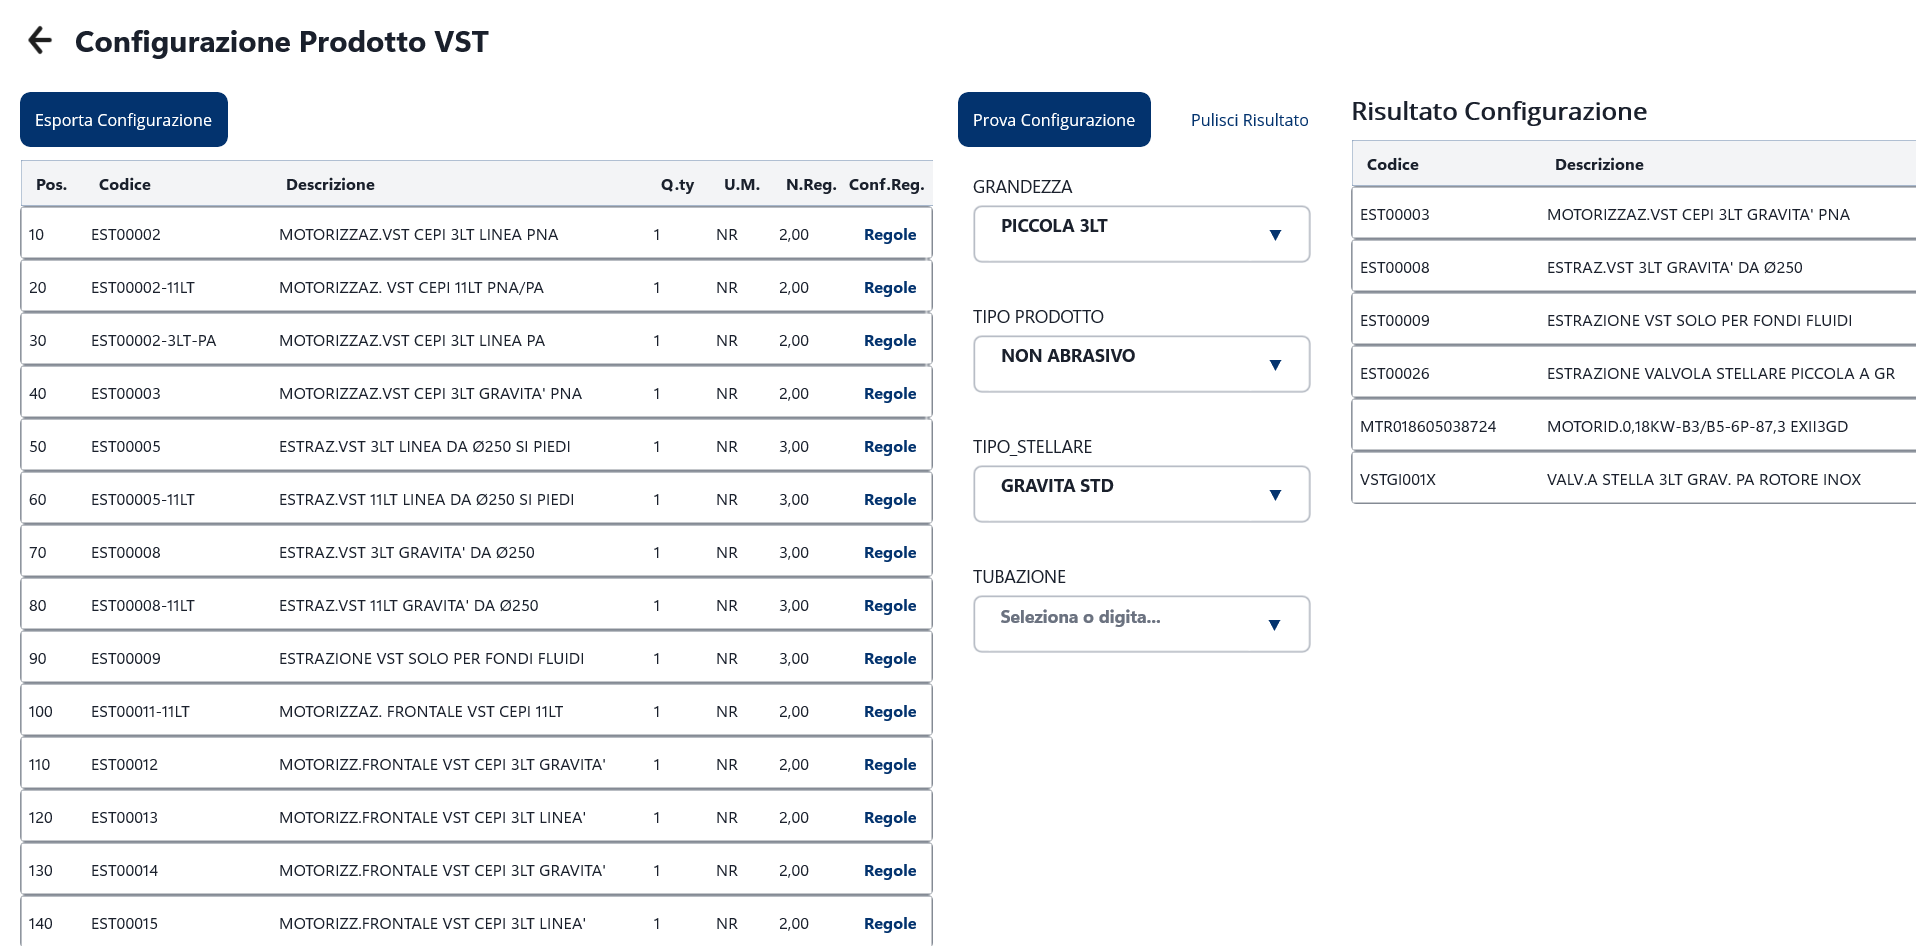
\includegraphics[width=0.9\linewidth]{figures/TestConfigurazione.png}}
    \caption{Test regole lato amministratore}\label{fig:Test regole lato amministratore}
\end{figure}

\chapter{Conclusioni}
Il presente lavoro di tesi, ha permesso di affrontare l'intero ciclo
di sviluppo del software. Sono stati curati tutti gli aspetti,
dalla raccolta dei requisiti e dalla progettazione dell'architettura fino alla
realizzazione del Model e della View.
L'obiettivo principale è stato creare un programma
di vendita che potesse sostituire l'attuale sistema. La raccolta dei requisiti è stata fondamentale per comprendere
le necessità degli utenti e le funzionalità richieste, ma
anche per definire cosa non fosse necessario implementare. La presenza dell'autore come 
dipendente in azienda ha rappresentato un vantaggio
significativo per il progetto, permettendo al contempo di sfruttare le conoscenze
pregresse e di interfacciarsi direttamente con gli utenti finali.
Quest'ultimo aspetto ha guidato la scelta della progettazione agile,
che ha permesso di avanzare iterativamente e raccogliere feedback continui dagli utenti.
L'applicativo è stato sviluppato utilizzando il framework
\dotnet{} in tutti gli strati della soluzione. Esso gestisce infatti, mediante \ac{EF Core},
la logica di business e di accesso ai dati e mediante \maui{},
la presentazione grafica.
Tale sistema offre inoltre la possibilità di creare applicazioni cross-platform.
Tra i vantaggi riscontrati nel mantenere un unico framework vi è la possibilità
di condividere il codice tra i diversi strati dell'applicazione,
semplificando lo sviluppo e la manutenzione del software. L'ambiente \dotnet{} ha offerto inoltre una vasta 
gamma di librerie e strumenti che,
attraverso l'uso di \nuget{}, hanno permesso nelle ultime fasi progettuali di
integrare moduli aggiuntivi come la generazione di report. La progettazione del database, attraverso l'utilizzo di \ac{SSIS},
ha consentito di costruire la struttura dati con metodologie professionali,
garantendo la possibilità di apportare modifiche in modo agile.
Nel modulo di interfaccia al database, la scrittura degli Unit Test
ha richiesto in una prima fase un notevole sforzo, ma ha permesso di individuare
e correggere tempestivamente eventuali errori o incongruenze nel codice.
Le modifiche al database sono state costantemente validate dai test, prima
di procedere all'aggiornamento degli strati superiori, garantendo la stabilità e
l'affidabilità del sistema. La realizzazione delle interfacce grafiche è stata
facilitata dall'utilizzo del pattern Factory. Le classi di utilità per i componenti grafici,
hanno permesso di sviluppare agevolmente nuovi ambienti,
mantenendo la coerenza visiva e funzionale dell'applicazione.
Parallelamente, l'adozione del pattern \ac{MVVM} ha consentito di separare
la logica di presentazione dalla logica di business, migliorando la manutenibilità
e facilitando la gestione degli eventi attraverso il data binding.
Allo stato attuale l'applicazione è prossima a un primo rilascio.
Nella versione desktop è già possibile eseguire l'intero ciclo di vendita,
consentendo all'utente finale di:
\begin{enumerate}
    \item accedere al programma tramite autenticazione;
    \item cercare o creare un nuovo cliente;
    \item generare un preventivo personalizzato in base alle esigenze del cliente;
    \item generare eventuali versioni alternative del preventivo;
    \item creare un report in formato PDF del preventivo;
    \item convertire il preventivo confermato in un ordine di vendita;
    \item associare una destinazione di consegna all'ordine di vendita.
\end{enumerate}
Per quanto riguarda la parte amministrativa,
l'applicazione consente, oltre a quanto sopra descritto,
di gestire i prodotti, creare configurazioni, modificare le tabelle con i
dati precompilati destinati agli utenti finali e infine amministrare i permessi
di accesso al programma. Negli sviluppi futuri si prevede di realizzare le interfacce grafiche per
la parte mobile e di implementare un database locale SQLite,
in modo da utilizzare l'applicazione anche in modalità offline.
Ulteriori sviluppi saranno affrontati sulla base dei feedback successivi
ai primi rilasci.

%----------------------------------------------------------------------------------------
% BIBLIOGRAPHY
%----------------------------------------------------------------------------------------

%\backmatter{}

%\nocite{*} % Remove this as soon as you have the first citation
\bibliographystyle{plain}
\bibliography{./Reference/references.bib}

% --- Inizio delle Appendici ---
\appendix

% Inclusione del file esterno
\chapter{Domande per i gruppi di analisi}\label{app:domande}
In questa appendice sono riportate le domande utilizzate per le interviste ai gruppi di analisi,
 sia per gli utilizzatori assidui del configuratore commerciale che per i non utilizzatori.
  Le domande sono state progettate per raccogliere informazioni sulle esperienze degli utenti,
   le loro aspettative e i suggerimenti per migliorare il nuovo configuratore commerciale e i contratti associati.
\section{Domande per i gruppi di analisi}
\subsection{Domande per entrambi i gruppi}
\begin{itemize}
    \item Anni di esperienza del tuo ruolo?
    \item Cosa ti aspetti dal nuovo configuratore commerciale e dai nuovi contratti?
    \item Quali sono le funzionalità attuali più importanti per te?
    \item Hai suggerimenti per future funzionalità da includere?
    \item Suggerimenti per facilitare l'adozione del nuovo configuratore?
\end{itemize}

\subsection{Domande per utilizzatori assidui}
\begin{itemize}
    \item Quali utilizzi fai dell'attuale programma Access?
    \item Mostrami un esempio di come utilizzi il configuratore commerciale.
    \item Quali sono le funzionalità che usi più frequentemente?
    \item Quali sono le funzionalità che trovi meno utili o difficili da usare?
    \item Quali sono le principali difficoltà che incontri nell'uso quotidiano?
    \item Quali operazioni pensi che richiedano più tempo o passaggi rispetto alle
          procedure che vorresti adottare?
    \item Puoi descrivere la procedura che hai in mente?
\end{itemize}

\subsection{Domande per non utilizzatori}
\begin{itemize}
    \item Come utilizzi attualmente i contratti commerciali nel tuo ruolo?
    \item Come ti approcci con il reparto vendite?
    \item Nel tuo ruolo hai bisogno di utilizzare direttamente il configuratore
          commerciale?
    \item Raccontami come ti approcci alla gestione dei contratti dopo che arrivano nel
          tuo reparto.
    \item Suggerimenti per facilitare l'adozione del nuovo configuratore?
\end{itemize}
\chapter{Trascrizione interviste con i soci aziendali}\label{app:risultati-interviste-proprieta} % Verificare se "proprietà" è il termine voluto
In questa appendice sono riportate le trascrizioni delle interviste effettuate ai soci dell'azienda,
al fine di raccogliere informazioni sulle esigenze e le problematiche attuali del sistema di preventivazione.
\section{Situazione attuale e problematiche}
Attualmente l'ufficio commerciale utilizza un database Microsoft Access, in uso da
oltre 20 anni.
\begin{itemize}
      \item \textbf{Punti di forza:} Estrema velocità di inserimento per utenti esperti; personalizzazione
            storica delle stampe e delle logiche.
      \item \textbf{Volume dati:} Circa 6 offerte/giorno per utente (commesse) e 18/giorno (ricambi/\ac{RA}).
            Totale annuo stimato: \(>2200\) offerte commesse.
      \item \textbf{Limitazioni critiche:}
            \begin{itemize}
                  \item Mancanza di integrazione con il gestionale \ac{ERP} (Ad Hoc).
                  \item Necessità di reinserimento dati manuale da Offerta a Ordine (doppio lavoro).
                  \item Gestione prezzi manuale o basata sull'esperienza (non collegata al costo
                        industriale aggiornato).
            \end{itemize}
\end{itemize}

\section{Criticità rilevate}
\subsection{Disallineamento tecnico-commerciale}
Attualmente, una volta firmato il contratto commerciale, le modifiche tecniche (\ac{PM}/\ac{UT})
non vengono tracciate nel sistema di preventivazione.
\begin{itemize}
      \item \textbf{Conseguenza:} Per replicare un impianto o vendere ricambi corretti, il commerciale
            deve consultare gli schemi CAD/Tecnici e il gestionale,
            poiché l'offerta originale in Access diventa obsoleta/inaccurata dopo la conferma d'ordine.
      \item \textbf{Rischio:} Vendita di ricambi errati o incoerenze nelle offerte copiando vecchie offerte
            per recuperare informazioni, condizioni e note.
\end{itemize}

\subsection{Inefficienza gestione ricambi (Spare Parts)}
Il flusso per i ricambi è eccessivamente complesso rispetto al valore economico.
\begin{itemize}
      \item \textbf{Situazione attuale:} L'Area Manager deve aprire una nuova offerta da zero o copiare
            vecchie offerte, richiedere
            quotazioni interne se non già presenti, attendere risposte e infine emettere l'offerta.
            Dopo la conferma del cliente, deve trasformarla in ordine.
      \item \textbf{Collo di bottiglia:} Troppi passaggi (Commerciali → Ufficio Tecnico → Pricing Office → Offerta).
      \item \textbf{Obiettivo:} Ridurre drasticamente i tempi per rendere profittevole la vendita proattiva,
            che ad oggi non viene effettuata.
\end{itemize}

\section{Requisiti funzionali emersi}

\subsection{Gestione offerte e configuratore}
Il sistema deve guidare l'utente, specialmente se junior, nella composizione
dell'impianto.
\begin{itemize}
      \item \textbf{Selezione guidata:} Selezionando un macro-componente (es. ``Trasporto Pneumatico'' o ``STX''),
            il sistema deve proporre in automatico gli accessori correlati (filtri, valvole, compressori) tramite menù a tendina.
      \item \textbf{Alert di completezza:} Avvisi automatici in caso di macchine essenziali mancanti
            (es. ``Hai inserito il trasporto, ma manca il compressore'').
      \item \textbf{Template per applicazione:} Possibilità di richiamare configurazioni standard (Template di impianto)
            basate sul prodotto finale del cliente (es. ``Linea Pan di Spagna'', ``Linea Biscotti'') e non solo sul nome cliente.
\end{itemize}

\subsection{Listini e pricing}
\begin{itemize}
      \item \textbf{Automazione costi:} Il prezzo di vendita deve scaturire automaticamente dal costo industriale
            aggiornato (integrazione con il gestionale), applicando regole di ricarico predefinite.
      \item \textbf{Eliminazione colli di bottiglia:} Il commerciale non deve dover chiedere quotazioni interne per
            componentistica standard.
\end{itemize}

\subsection{Gestione flusso obbligatorio ordine e revisioni}
\begin{itemize}
      \item \textbf{Integrazione ERP:} Passaggio automatico da ``Offerta Confermata''
            a ``Ordine Gestionale'' senza reinserimento dati.
      \item \textbf{Doppio contratto (Versionamento):}
            \begin{enumerate}
                  \item \textbf{Contratto commerciale:} La versione firmata dal cliente (congelata).
                  \item \textbf{Contratto tecnico (``As-Built''):} Una copia viva che viene modificata dai
                        PM/Ufficio Tecnico durante la realizzazione.
                        Questa diventerà la base per le future assistenze e i ricambi.
            \end{enumerate}
\end{itemize}

\subsection{Distinzione flussi di lavoro}
Il software deve distinguere a monte la tipologia di richiesta per instradare
il lavoro:
\begin{enumerate}
      \item \textbf{Nuovi impianti / commesse:} Flusso standard completo.
      \item \textbf{Ampliamenti:} Collegati a commesse esistenti ma gestiti dai commerciali.
      \item \textbf{Ricambi (spare parts):} Flusso semplificato e rapido. Accesso allo storico installato.
\end{enumerate}

\section{Requisiti non funzionali}
\begin{itemize}
      \item \textbf{Modalità offline:} Fondamentale per gli Area Manager in viaggio in zone
            con scarsa connettività.
            Sincronizzazione al rientro o via \ac{VPN}.
      \item \textbf{Multilingua:} Gestione avanzata delle descrizioni (necessità di una via di mezzo tra la descrizione
            ``estesa'' attuale, troppo lunga, e quella ``breve'', troppo criptica).
      \item \textbf{Velocità:} L'interfaccia non deve rallentare l'operatività dell'utente.
\end{itemize}
\chapter{Trascrizione utilizzatori}\label{app:risultati-interviste-utilizzatori}
In questa appendice sono riportate le trascrizioni delle interviste condotte con gli utilizzatori abituali
del sistema attuale, al fine di raccogliere i requisiti per il nuovo software.

\section{Operazioni comuni}
Le operazioni più comuni svolte all'interno dell'applicativo includono:
\begin{itemize}
      \item Creazione di offerte per ricambi e assistenza (\ac{RA}).
      \item Creazione di offerte per clienti non diretti.
      \item Creazione delle offerte Access per conto di agenti o rivenditori esterni.
      \item Creazione di offerte per clienti diretti.
      \item Creazione degli ordini ogni qualvolta un'offerta viene accettata.
      \item Ricerca e copia di vecchie offerte simili durante la creazione di nuove offerte.
      \item Correzione delle traduzioni preimpostate fornite da Access.
\end{itemize}

\section{Gestione protezione dati e accessi}
\subsection{Gestione utenti e visibilità degli agenti}
Per quanto riguarda la gestione degli utenti e la visibilità dei dati, gli agenti
hanno evidenziato i seguenti punti chiave:
\begin{itemize}
      \item \textbf{Segregazione dei dati:} È fondamentale mantenere la distinzione tra offerte e
            \ac{RA} (Richieste assistenza/ricambi).
            La distinzione tra i due tipi aiuta a evitare confusione e garantisce che le operazioni
            siano gestite correttamente.
      \item \textbf{Privacy per autore:} Un agente esterno non deve vedere i progetti o le offerte
            degli altri agenti per evitare conflitti di interesse (Policy aziendale).
      \item \textbf{Anagrafica clienti condivisa:} A differenza delle offerte, l'elenco clienti deve
            essere visibile a tutti, poiché può capitare di fare offerte per conto di altri commerciali.
\end{itemize}

\section{Flussi di lavoro attuali}

\subsection{Ricambi e assistenza post-vendita}
Il flusso di lavoro attuale, per la gestione dei ricambi e dell'assistenza
post-vendita, presenta diverse inefficienze dovute alla frammentazione degli strumenti
e alla mancanza di dati strutturati.

\begin{itemize}
      \item \textbf{Template di partenza:} Attualmente non esiste un template dedicato; si parte quindi
            da vecchi ordini e per individuare quali siano le assistenze, l'unica discriminante è
            l'autore.
            Questa pratica permette di ereditare tutte le condizioni di vendita e i dati del cliente,
            risparmiando tempo nella compilazione (operazione attualmente molto onerosa in termini di tempo).
      \item \textbf{Ricerca ricambi manuale:} L'operatore deve consultare disegni tecnici (Fusion, PDF, cartacei)
            e database separati (Access, Ad-Hoc, Excel, Server ``Commesse'') per identificare i codici dei ricambi.
      \item \textbf{Inserimento del componente:} Una volta individuato il componente, non essendoci una
            corrispondenza univoca dei codici, l'operatore deve trovare la corrispondenza in
            Access o creare un nuovo codice per il ricambio.
      \item \textbf{Creazione offerta complessa:} Non è facile né la ricerca né l'assegnazione di un prezzo
            se il componente è datato; la compilazione dell'offerta talvolta richiede calcoli manuali (prezzi, pesi, volumi).
            Spesso si ricorre alla copia di vecchie offerte \ac{RA} o commesse, pratica che trascina errori pregressi.
\end{itemize}

\subsection{Impianti nuovi e ampliamenti}
L'attuale processo di creazione delle offerte prevede i seguenti passaggi:
\begin{enumerate}
      \item \textbf{Raccolta requisiti:} Il commerciale si interfaccia con il cliente per comprendere le
            esigenze tecniche e commerciali.
      \item \textbf{Ricerca e copiatura di una vecchia offerta:} Spesso si parte da un'offerta precedente simile
            per velocizzare il processo.
      \item \textbf{Selezione prodotti:} Aggiunta manuale dei prodotti, uno a uno, tramite descrizione.
      \item \textbf{Configurazione offerta:} Creazione dell'offerta suddivisa in capitoli, applicando gli sconti
            e i calcoli necessari.
      \item \textbf{Invio al cliente:} Generazione del documento finale in formato PDF o cartaceo e invio al cliente.
      \item \textbf{Approvazione offerta:} In caso di accettazione, si procede con la conferma d'ordine e
            la comunicazione all'ufficio produzione e all'ufficio amministrativo.
\end{enumerate}

\section{Problemi attuali del sistema}
Dall'intervista i commerciali hanno fatto emergere le seguenti criticità del sistema attuale:
\begin{itemize}
      \item \textbf{Lentezza e complessità:} L'intero processo di gestione è lento e laborioso
            e richiede molto tempo per completare un'offerta. Questo è dovuto alla necessità di consultare molteplici fonti di
            dati non integrate. Il programma stesso utilizzato (Access) risulta lento e macchinoso, con molti tempi morti.
      \item \textbf{Disallineamento codici:} Esiste una discrepanza tra i codici commerciali e quelli tecnici/gestionali.
            Questo costringe a ricerche manuali su schemi funzionali o database separati per identificare il pezzo corretto (Ad-Hoc, Fusion, \dots).
      \item \textbf{Mancanza di automazione nei calcoli:}
            \begin{itemize}
                  \item \textbf{Prezzi:} I costi e i prezzi di vendita devono essere spesso calcolati manualmente o verificati
                        su Excel/Ad-Hoc, specialmente per componenti su misura o obsoleti.
                  \item \textbf{Logistica:} Non esiste un calcolo automatico di volumi e pesi per il trasporto; l'utente deve
                        ipotizzare i dati basandosi su vecchi DDT o sull'esperienza. Il costo è talvolta calcolato mediante il sito del corriere.
                  \item \textbf{Manodopera:} I tempi e i costi per gli interventi tecnici (es: sostituzione saccone) non sono
                        standardizzati e richiedono consultazioni continue con i colleghi (es: Logistica).
            \end{itemize}
      \item \textbf{Componenti elettrici:} La gestione e l'inserimento di materiale elettrico sono molto difficili per la 
      complessità e la varietà di codici esistenti. Attualmente si consulta direttamente l'ufficio tecnico elettrico per
            avere un elenco dei componenti necessari da offrire.
      \item \textbf{Gestione obsolescenza:} È difficile sapere se un componente venduto anni fa è stato sostituito da una
            nuova versione o se è obsoleto, rischiando di vendere pezzi non più procurabili. Serve un sistema di tracciamento delle
            sostituzioni e delle obsolescenze (es. Fusion).
      \item \textbf{Discrepanza ``As Built'':} Le modifiche fatte in cantiere (\ac{RA} di cantiere) o successive alla vendita non
            sono sempre tracciate in modo unitario, rendendo difficile conoscere la configurazione reale dell'impianto attuale, punto
            fondamentale per una corretta assistenza senza errori.
      \item \textbf{Sistema di traduzione:} È fondamentale avere un sistema di traduzione
            integrato e affidabile per le descrizioni
            dei componenti e delle offerte; attualmente, oltre alle traduzioni preimpostate di Access
            (spesso da correggere), si utilizzano
            servizi esterni (Google Translate) che richiedono tempo e possono introdurre errori.
\end{itemize}

\section{Requisiti Funzionali per il nuovo software}

\subsection{Database e integrazione}
Per migliorare l'integrazione dei dati e la gestione delle informazioni, il nuovo sistema deve prevedere:
\begin{itemize}
      \item \textbf{Database unificato:} Il nuovo sistema deve integrare o dialogare con Ad-Hoc \ac{ERP}, Fusion \ac{PLM}
            e l'archivio storico per garantire l'univocità del dato.
      \item \textbf{Codifica condivisa:} Allineamento tra codici commerciali e tecnici.
            Il codice usato per l'offerta deve permettere di risalire automaticamente a costi, distinta base e disegni.
      \item \textbf{Gestione revisioni:} Il sistema deve tracciare le revisioni dei clienti
            (cambi nome, stabilimento) e dei componenti (sostituzioni, obsolescenza).
      \item \textbf{Codici a catalogo:} Il sistema deve già contenere tutti i codici esistenti;
            la volontà del commerciale è di non doverli inserire manualmente. È necessario prevedere una
            gestione esterna dedicata all'aggiunta e all'aggiornamento di nuovi codici.
      \item \textbf{Integrazione nel flusso dell'ordine:} Attualmente esistono 3 codici fondamentali per
            la gestione dell'ordine:
            \begin{itemize}
                  \item \textbf{Codice offerta:} Codice univoco dell'offerta commerciale.
                  \item \textbf{Codice ordine:} Codice univoco dell'offerta trasformata in ordine.
                  \item \textbf{Codice distinta:} Codice univoco della distinta base gestionale dell'ordine.
            \end{itemize}
            Il nuovo sistema deve collegare e mostrare questi 3 codici in modo chiaro e visibile per l'operatore,
            facilitando le ricerche e la tracciabilità dell'ordine.
\end{itemize}

\subsection{Ricerca e navigazione ricambi}
Per facilitare la ricerca e la selezione dei ricambi, il sistema deve prevedere:
\begin{itemize}
      \item \textbf{Ricerca multicriterio:} Necessità di cercare per Numero di Commessa (fondamentale),
            Cliente, Stabilimento e Tag Tecnici (es: ``valvola a farfalla'').
      \item \textbf{Struttura ad albero/gerarchica:} Possibilità di esplorare la distinta base \ac{BOM}
            scendendo nei livelli (esplosione componenti) per individuare il singolo ricambio.
      \item \textbf{Filtri per ``Ricambi tipici'':} Implementazione di filtri che mostrino, per una data
            famiglia di macchine (es. Lift, Vibrovaglio), solo i componenti tipicamente venduti come ricambi;
            i codici devono essere allineati ai codici tecnici, velocizzando l'assistenza una volta individuato il componente.
\end{itemize}

\subsection{Creazione e gestione offerte}
Per semplificare e velocizzare la creazione delle offerte di ricambi e assistenza, il sistema deve prevedere:
\begin{itemize}
      \item \textbf{Automazione descrizioni e lingue:} Compilazione automatica delle descrizioni in lingua
            (traduzioni pre-caricate) senza dover usare traduttori esterni.
      \item \textbf{Calcolo prezzi automatizzato:} Il sistema deve recuperare il costo industriale da Ad-Hoc e
            applicare le maggiorazioni o i listini specifici per cliente/settore.
      \item \textbf{Tracciabilità univoca della pratica:} Mantenimento di un riferimento univoco che segua
            la pratica dalla richiesta iniziale all'ordine confermato, per evitare duplicazioni e facilitare la
            rintracciabilità, affiancato da uno stato di avanzamento \textit{(es. ``In Revisione'', ``Inviata'', ``Accettata'',
                  ``Rifiutata'')} per facilitarne l'interpretazione.
      \item \textbf{Distinzione tipologie RA:} Gestione differenziata ma tracciabile per ``Ricambi'',
            ``Ampliamenti'' e ``RA di Cantiere''. Al momento le assistenze sopra citate sono raggruppate sotto
            l'unico cappello del ``VSS''.
\end{itemize}

\subsection{Funzionalità avanzate e UX}
Per migliorare l'esperienza utente e l'efficienza operativa, il sistema deve prevedere:
\begin{itemize}
      \item \textbf{Intestazione offerta e dati cliente:} È importante riportare tutte le informazioni
            attuali del cliente (Indirizzo, Nome, Numero di commessa associata) in modo chiaro e visibile nella
            schermata dell'offerta.
      \item \textbf{Schermata dedicata allo storico:} Una sezione dove poter visualizzare tutte le offerte
            e gli ordini precedenti associati al cliente o alla commessa selezionata.
      \item \textbf{Schermata offerta intuitiva:} Interfaccia user-friendly che guidi l'utente passo-passo
            nella compilazione dell'offerta, minimizzando errori e omissioni.
      \item \textbf{Visualizzazione dati completa:} Interfaccia che mostri tutte le informazioni rilevanti
            (es: dettagli tecnici completi come ``filtrante/non filtrante'') senza dover scorrere o aprire popup.
      \item \textbf{Modalità offline/sync:} Il software deve permettere di lavorare in locale (offline) durante le visite dai clienti
            e sincronizzarsi automaticamente con il database centrale una volta ristabilita la connessione \ac{VPN}.
      \item \textbf{Multi-finestra:} Possibilità di tenere aperte più schede o finestre di offerte diverse contemporaneamente.
            Utile la possibilità di un sistema multi-documento \textit{(es. AutoCAD)}.
      \item \textbf{Interfaccia mobile/tablet:} Ottimizzazione per l'uso su tablet (iPad) per la compilazione
            di dati preliminari e note durante il sopralluogo o in fiera.
\end{itemize}

\section{Note di implementazione}
Gli utilizzatori hanno fornito alcune indicazioni utili per la fase di implementazione:
\begin{itemize}
      \item \textbf{Campi obbligatori:} Rendere obbligatoria la distinzione tra ``Ampliamento'' e ``Ricambi''
            (attualmente campo discrezionale spesso vuoto)
            per migliorare la ricercabilità futura.
      \item \textbf{Beta tester:} Si consiglia di iniziare la fase di test con figure
            tecniche/analitiche e commerciali esperti.
      \item \textbf{Transizione:} Prevista una fase transitoria con utilizzo parallelo dei due sistemi;
            necessaria migrazione o accessibilità facile ai dati storici.
\end{itemize}

\section{Numeri utili}
Per capire gli attuali tempi di lavoro e il volume storico di offerte gestite, si riportano i seguenti dati:
\begin{itemize}
      \item \textbf{Offerte VS Ordini:} Attualmente a sistema risultano create (o presenti nello storico \ac{RA})
            circa 57.000 offerte (\ac{RA}), di cui circa 41.000 si sono trasformate in ordini effettivi.
      \item \textbf{Tempo base per una semplice offerta:} Attualmente, per una richiesta tipo di cui si conoscono già
            il numero di commessa e i codici da inserire, il tempo medio per la creazione di un'offerta è di circa 15 minuti.
            Il tempo sale notevolmente se devono essere ricercate le informazioni mancanti.
\end{itemize}
\chapter{Trascrizione non utilizzatori}\label{app:risultati-interviste-non-utilizzatori}
In questa appendice sono riportate le trascrizioni delle interviste effettuate
ai non utilizzatori del sistema di vendite attuale.
Le interviste hanno avuto l'obiettivo di raccogliere informazioni sulle esigenze odierne
e future del sistema di preventivazione.
\section{Ruoli coinvolti e utilizzo attuale degli strumenti}
I reparti tecnici, di gestione commessa e logistici interagiscono in modo indiretto
o marginale con l'attuale database Microsoft Access, basandosi prevalentemente su passaggi cartacei o file esterni:
\begin{itemize}
      \item \textbf{Ufficio Project Management e Project Engineering:} Coordinano le commesse tra commerciale
            e reparti tecnici, definendo le specifiche e supervisionando installazione e post-vendita.
            Non utilizzano Access; consultano i contratti in formato cartaceo o scansionato per revisionare le
            specifiche tecniche e contattare i clienti.
      \item \textbf{Ufficio Tecnico Meccanico:} Si occupa della progettazione meccanica e dei disegni costruttivi.
            Non utilizza Access; recepisce le specifiche dal cartaceo tramite i \ac{PE} per verificare revisioni,
            limiti dei componenti e condizioni del sito di montaggio.
      \item \textbf{Ufficio Tecnico Elettrico:} Gestisce la progettazione di quadri e impianti elettrici.
            Attualmente sopperisce alle carenze del sistema utilizzando fogli Excel esterni
            per il dimensionamento/calcolo costi
            (\textit{QUAEL.xltm}) e per la validazione tecnica dei preventivi (\textit{PROGETTO CEPI-Scheda progetto r2.xlsx}).
      \item \textbf{Ufficio Logistica:} Gestisce spedizioni, dogane e trasporti. Utilizza Access solo marginalmente
            per verificare
            le date di consegna o correggere a valle indirizzi, causali, dati di trasporto e Incoterms.
            L'operatività ruota attorno
            a un
            ``File Logistico'' in Excel centralizzato e alla gestione di copie cartacee nelle cartelle di rete.
      \item \textbf{Ufficio Manualistica e Ufficio Acquisti:} La Manualistica redige manuali e certificazioni dei prodotti venduti;
            l'Ufficio Acquisti gestisce gli ordini ai fornitori e controlla i contratti commerciali per verificare i ricambi in
            assistenza ed eventuali discrepanze tecniche o commerciali.
\end{itemize}

\section{Criticità trasversali rilevate}

\subsection{Frammentazione documentale e supporto cartaceo}
\begin{itemize}
      \item \textbf{Disallineamento delle informazioni:} L'utilizzo di copie cartacee multiple (distribuite tra Vendite,
            Ufficio Tecnico, Elettrico e Logistica) e di annotazioni manuali sul cartaceo comporta la perdita di informazioni e
            la circolazione di versioni obsolete.
      \item \textbf{Duplicazione per tempistiche differenti:} Per le commesse miste (meccaniche ed elettriche),
            la Logistica è costretta a duplicare fisicamente le copie tecniche delle \ac{RA} per gestire le diverse
            tempistiche dei due uffici.
\end{itemize}

\subsection{Disconnessione anagrafica ed errori di input}
\begin{itemize}
      \item \textbf{Disallineamento Access vs Ad Hoc:} Access presenta anagrafiche spesso non aggiornate e prive
            di storicizzazione, mentre l'ERP Ad Hoc contiene i dati fiscali corretti (Sede Legale) ma risulta
            impreciso sulle sedi operative o di spedizione.
      \item \textbf{Propagazione degli errori:} La prassi commerciale di duplicare vecchie commesse/RA trascina errori
            pregressi che devono essere corretti manualmente dalla Logistica a valle del processo.
      \item \textbf{Omissione dati logistici:} Nelle offerte mancano quasi sempre informazioni essenziali per il
            trasporto quali Incoterms, tipologia di imballo, pesi e volumi.
\end{itemize}

\subsection{Gestione post-vendita e disallineamento per le dogane}
\begin{itemize}
      \item \textbf{Variazioni non tracciate:} Il metodo attuale punta alla vendita rapida,
            ma non traccia in modo strutturato i componenti aggiunti o modificati in fase di progettazione e realizzazione.
      \item \textbf{Criticità sulle Packing List doganali:} I commerciali vendono ``macro-codici'' (es: impianto completo),
            ma le dogane (specialmente extra-UE) esigono il dettaglio di ogni singolo pallet. Poiché il sistema non
            esplode i macro-codici nei colli fisici, l'associazione tra voci contrattuali, distinta tecnica e pallet preparati
            dagli spedizionieri avviene manualmente, generando un alto rischio di errori doganali.
\end{itemize}

\section{Requisiti funzionali emersi}

\subsection{Struttura del contratto, distinta base e codifica}
\begin{itemize}
      \item \textbf{Gestione per macro-codici e standardizzazione:}
            \begin{itemize}
                  \item Utilizzo di ``macro-codici'' contenitore in fase di vendita (es. \textit{Macro-codice Quadro},
                        \textit{Pannello Operatore}, \textit{TVB generico}) direttamente agganciati alla distinta base
                        (completa al 90\%), che l'Ufficio Tecnico completerà poi con i disegni specifici.
                  \item Spinta verso la ``standardizzazione a catalogo'' tramite l'analisi statistica dei \textit{Best Sellers}
                        (es. TVB standard, stellari taglie 1000/1500/2000), facendo coincidere il codice di vendita con quello di realizzazione
                        e separando il flusso standard da quello ``fuori standard''.
                  \item Allineamento univoco dei codici articolo tra il nuovo configuratore e il gestionale Ad Hoc.
            \end{itemize}
      \item \textbf{Separazione ed esplosione delle voci (Meccanica vs Elettrica):}
            \begin{itemize}
                  \item Creazione di due sezioni contrattuali ben distinte per i componenti meccanici e quelli elettrici,
                        superando la confusione attuale.
                  \item Esplosione automatica: l'inserimento di utenze meccaniche (es: motori, vibratori) deve generare
                        automaticamente le voci elettriche correlate nel contratto tecnico (es: gli inverter devono essere integrati
                        nel quadro o associati all'utenza specifica, non trattati come voci isolate).
            \end{itemize}
      \item \textbf{Rintracciabilità e collegamento logistico:}
            \begin{itemize}
                  \item Superamento dei codici generici per garantire la tracciabilità dell'esatta variante del
                        componente venduto (es: variante specifica di un \textit{WP104}).
                  \item Collegamento nativo tra distinta commerciale e distinta tecnica (tramite Rif CC)
                        fin dalla progettazione, per automatizzare l'associazione con i pallet fisici e la generazione delle Packing List.
            \end{itemize}
\end{itemize}

\subsection{Configuratore tecnico, normativo e logistico}
Il sistema deve guidare il commerciale attraverso vincoli all'ingresso (menu a tendina) e controlli automatici
di completezza prima del salvataggio:
\begin{itemize}
      \item \textbf{Guida e vincoli per la parte elettrica:}
            \begin{itemize}
                  \item Suggerimento automatico del materiale del quadro in base alle utenze inserite (es: taglia corretta
                        dell'inverter in base ai motori venduti) e domande finali per proporre accessori consigliati.
                  \item Inserimento automatico di default dei sezionatori a bordo macchina per ogni motore.
                  \item Distinzione netta tra ``quadro nuovo'' e ``ampliamento'': in caso di ampliamento, il sistema deve
                        indicare la disponibilità di spazio fisico nel quadro esistente per evitare errori di valutazione e costi imprevisti.
                  \item Campi tecnici obbligatori: Paese di destinazione, alimentazione (es. 230V 50Hz, 400V 60Hz, DC/AC),
                        materiale del quadro (inox, verniciato), tipologia canaline (chiusa, forata), numero/tipologia utenze e
                        certificazioni (es. UL/USA, la cui selezione deve aggiornare in automatico componenti e costi).
            \end{itemize}
      \item \textbf{Specifiche per manualistica, meccanica e acquisti:}
            \begin{itemize}
                  \item Campi dedicati alle certificazioni richieste per i componenti venduti (CE, ATEX, FDA, ecc.)
                        e alle norme di riferimento per i prodotti acquistati da terzi (ATEX, alimentari, ecc.).
                  \item Valorizzazione dettagliata delle caratteristiche tecniche (dati elettrici dei motori, dati
                        meccanici, allestimenti, accessori) per agevolare la stesura dei manuali.
                  \item Verifica delle condizioni del luogo di montaggio per attivare controlli specifici sulle macchine
                        (es. Globosili esterni in zone sismiche), definire i trasporti e rilevare limitazioni d'uso dei componenti.
            \end{itemize}
      \item \textbf{Vincoli e alert logistici/doganali per Paese:}
            \begin{itemize}
                  \item Compilazione obbligatoria e guidata di Incoterms (DAP, DDP, FCA, ecc.), tipologia di imballo, pesi e volumi.
                  \item Generazione di alert automatici all'inserimento dell'ordine in base al Paese di destinazione per requisiti
                        di fumigazione/ISPM 15 sui pallet in legno (es: Brasile, Australia, Turchia), materiali proibiti
                        (es: ancoranti chimici vietati) e necessità di permessi eccezionali o montaggi.
            \end{itemize}
\end{itemize}

\subsection{Preventivazione, calcolo costi e varianti}
\begin{itemize}
      \item \textbf{Internalizzazione dei fogli di calcolo:} Integrazione nel software delle logiche di dimensionamento,
            calcolo costi e validazione preventiva oggi gestite sui file Excel esterni (\textit{QUAEL.xltm}
            e \textit{Scheda progetto r2.xlsx}).
      \item \textbf{Costificazione delle variazioni:} Possibilità per il Project Management di costificare le variazioni
            tecniche in modo separato dal contratto commerciale, così da valutare il margine di manovra sulle modifiche in corso d'opera.
\end{itemize}

\subsection{Gestione contrattuale, revisioni e ``As-Built''}
\begin{itemize}
      \item \textbf{Doppio contratto (Commerciale vs Tecnico):} Poiché il contratto commerciale firmato e sdoganato ha
            vincoli legali e non può essere alterato liberamente, il sistema deve gestire in parallelo un ``Contratto Tecnico''
            (copia speculare).
      \item \textbf{Allineamento Contratto vs Schema (P\&ID) e Feedback Loop:}
            \begin{itemize}
                  \item Sostituzione di note esterne e file Word con una sezione dedicata che registri le discrepanze tra
                        venduto commerciale ed eseguito tecnico (es: modifiche allo schema P\&ID, numero valvole, componenti extra),
                        mantenendo allineati i dati tecnici ed economici.
                  \item Implementazione di un sistema di feedback \textit{``As-Built''} per registrare le
                        modifiche effettive apportate durante la realizzazione, ottimizzando i processi e la precisione dei futuri preventivi.
                  \item Possibilità di riproporre al cliente il contratto tecnico aggiornato affinché diventi
                        il documento ufficiale.
            \end{itemize}
\end{itemize}

\subsection{Workflow, pianificazione temporale e notifiche}
\begin{itemize}
      \item \textbf{Monitoraggio date e colli di bottiglia:} Registrazione e confronto automatico
            tra la \textit{Data emissione ordine}
            (conferma cliente) e la \textit{Data stampa/presa in carico} (ricezione interna), evidenziando eventuali ritardi.
      \item \textbf{Pianificazione a ritroso (Back-Scheduling):} Calcolo automatico delle milestone intermedie a partire dalla
            \textit{Data di evasione} (spedizione prevista) o dallo \textit{Start-up impianto}
            per garantire il rispetto delle tempistiche.
      \item \textbf{Gestione stati e Alerting automatico:} Distinzione chiara degli stati della commessa
            (es: da \textit{Pre-inserimento / Bozza commerciale} a \textit{Inserito in Impianti / Validato tecnicamente}).
            Al cambio di stato, invio di notifiche automatiche (email o alert in-app) ai reparti a valle (es. Elettrico, Logistica),
            sostituendo il passaggio fisico del fascicolo cartaceo e le email manuali.
\end{itemize}

\section{Requisiti su anagrafiche, tracciabilità e governance}
\begin{itemize}
      \item \textbf{Tripla entità anagrafica e storicizzazione:}
            \begin{itemize}
                  \item Distinzione obbligatoria in anagrafica tra tre soggetti: \textit{Intestatario} (Fiscale),
                        \textit{Utilizzatore} (Fisico) e \textit{Destinatario Merce} (Logistico).
                  \item Storicizzazione dei dati anagrafici e introduzione di \textit{date di obsolescenza} per articoli
                        e sedi: in caso di cambio sede o P.IVA del cliente, i documenti storici (es. DDT passati) devono conservare
                        i dati validi all'epoca dell'emissione.
            \end{itemize}
      \item \textbf{Tracciabilità totale (Audit Log) e responsabilità:}
            \begin{itemize}
                  \item Eliminazione delle annotazioni su carta a favore di una visibilità digitale in tempo reale per tutti i
                        reparti autorizzati (Commerciale, \ac{UT}, \ac{PM}, Logistica, Magazzino).
                  \item Log completo delle modifiche ai dati di commessa che registri \textit{Chi} ha effettuato la variazione,
                        \textit{Quando} (timestamp) e \textit{Cosa} è cambiato (valore precedente vs valore attuale).
                  \item Presenza di un campo ``Compilato da'' autocompilato con l'utente loggato, ma mantenuto editabile
                        per gestire eventuali deleghe o correzioni di assegnazione.
            \end{itemize}
      \item \textbf{Governance Top-Down e formazione:}
            \begin{itemize}
                  \item Impostazione rigida del database: divieto di popolamento libero da parte degli utenti e definizione
                        delle regole a monte tramite un team ristretto per preservare l'integrità dei dati.
                  \item Formazione specifica per il reparto commerciale sull'utilizzo del nuovo sistema e sull'importanza
                        della correttezza dei dati inseriti a monte.
            \end{itemize}
\end{itemize}

\begin{acknowledgements}
    Desidero esprimere la mia più sincera gratitudine alla Prof.ssa Annalisa Franco per la guida,
    la disponibilità e il prezioso supporto forniti durante la stesura di questa tesi.
    Un sentito ringraziamento va a CEPI S.p.A., che mi ha offerto l'opportunità di conciliare
    il percorso lavorativo con quello universitario, consentendomi al tempo stesso di mettere in pratica
    le conoscenze acquisite nel corso degli studi.
    Un ringraziamento particolare è rivolto a Sandra Ceccarelli, che mi ha proposto questo progetto di tesi
    e mi ha accompagnato con disponibilità e competenza durante il suo sviluppo, insieme a Claudio Rossi,
    il cui supporto è stato altrettanto prezioso.
    Desidero inoltre ringraziare tutti i miei compagni di corso e i colleghi che, in questi tre anni, mi hanno sostenuto,
    aiutato e incoraggiato nei momenti più impegnativi di questo percorso.
    Dedico un ringrazimento anche a mio nonno, che ha creduto in me e lottato per esserci in questo momento così importante.
    Infine, il ringraziamento più importante è dedicato a Elisa. È stata lei a spronarmi a intraprendere questo cammino
    e ad accompagnarmi fino al traguardo finale. Mi è sempre stata accanto, sostenendomi con pazienza,
    comprensione e affetto in ogni fase del percorso. Senza il suo supporto non sarei riuscito a raggiungere
    questo importante obiettivo.
    Questo percorso universitario è stato impegnativo, ma al contempo estramamente gratificante
    lasciandomi nuove conoscenze sia professionali che personali. Mi ha fatto
    maturare e crescere, permettendomi di affrontare le sfide con maggiore sicurezza e determinazione.
    Per tutti questi motivi, le dedico questo lavoro e il traguardo che rappresenta.
\end{acknowledgements}

\end{document}
